\subsection{Компьютерные технологии}
	
	\subsubsection{Аннотация}

        Курс <<Компьютерные технологии>> имеет в основном отрицательные оценки.

        Лекции Ефанова Н.Н. получили смешанные отзывы. Студенты отметили, что лектор непонятно преподносит материал. Совет студентов и аспирантов ФРКТ просит передать эти сведения лектору.

        Семинарист Кулиев Р.С. получил негативные отзывы. Респонденты отметили, что преподаватель постоянно пропускает семинары и несвоевременно принимает задания. Совет студентов и аспирантов ФРКТ рекомендует заменить этого семинариста.

        Семинарист Чуканова О.В. получила негативные отзывы. Респонденты отметили, что семинарист не смог внятно рассказать материал курса. Совет студентов и аспирантов ФРКТ рекомендует заменить этого семинариста.

        Обобщая всё сказанное выше, Совет студентов и аспирантов ФРКТ рекомендует пересмотреть учебную программу всего курса.


	\subsubsection{Общий отзыв студентов о курсе}

		\begin{figure}[H]
			\centering
			\begin{subfigure}[b]{0.45\textwidth}
				\centering
				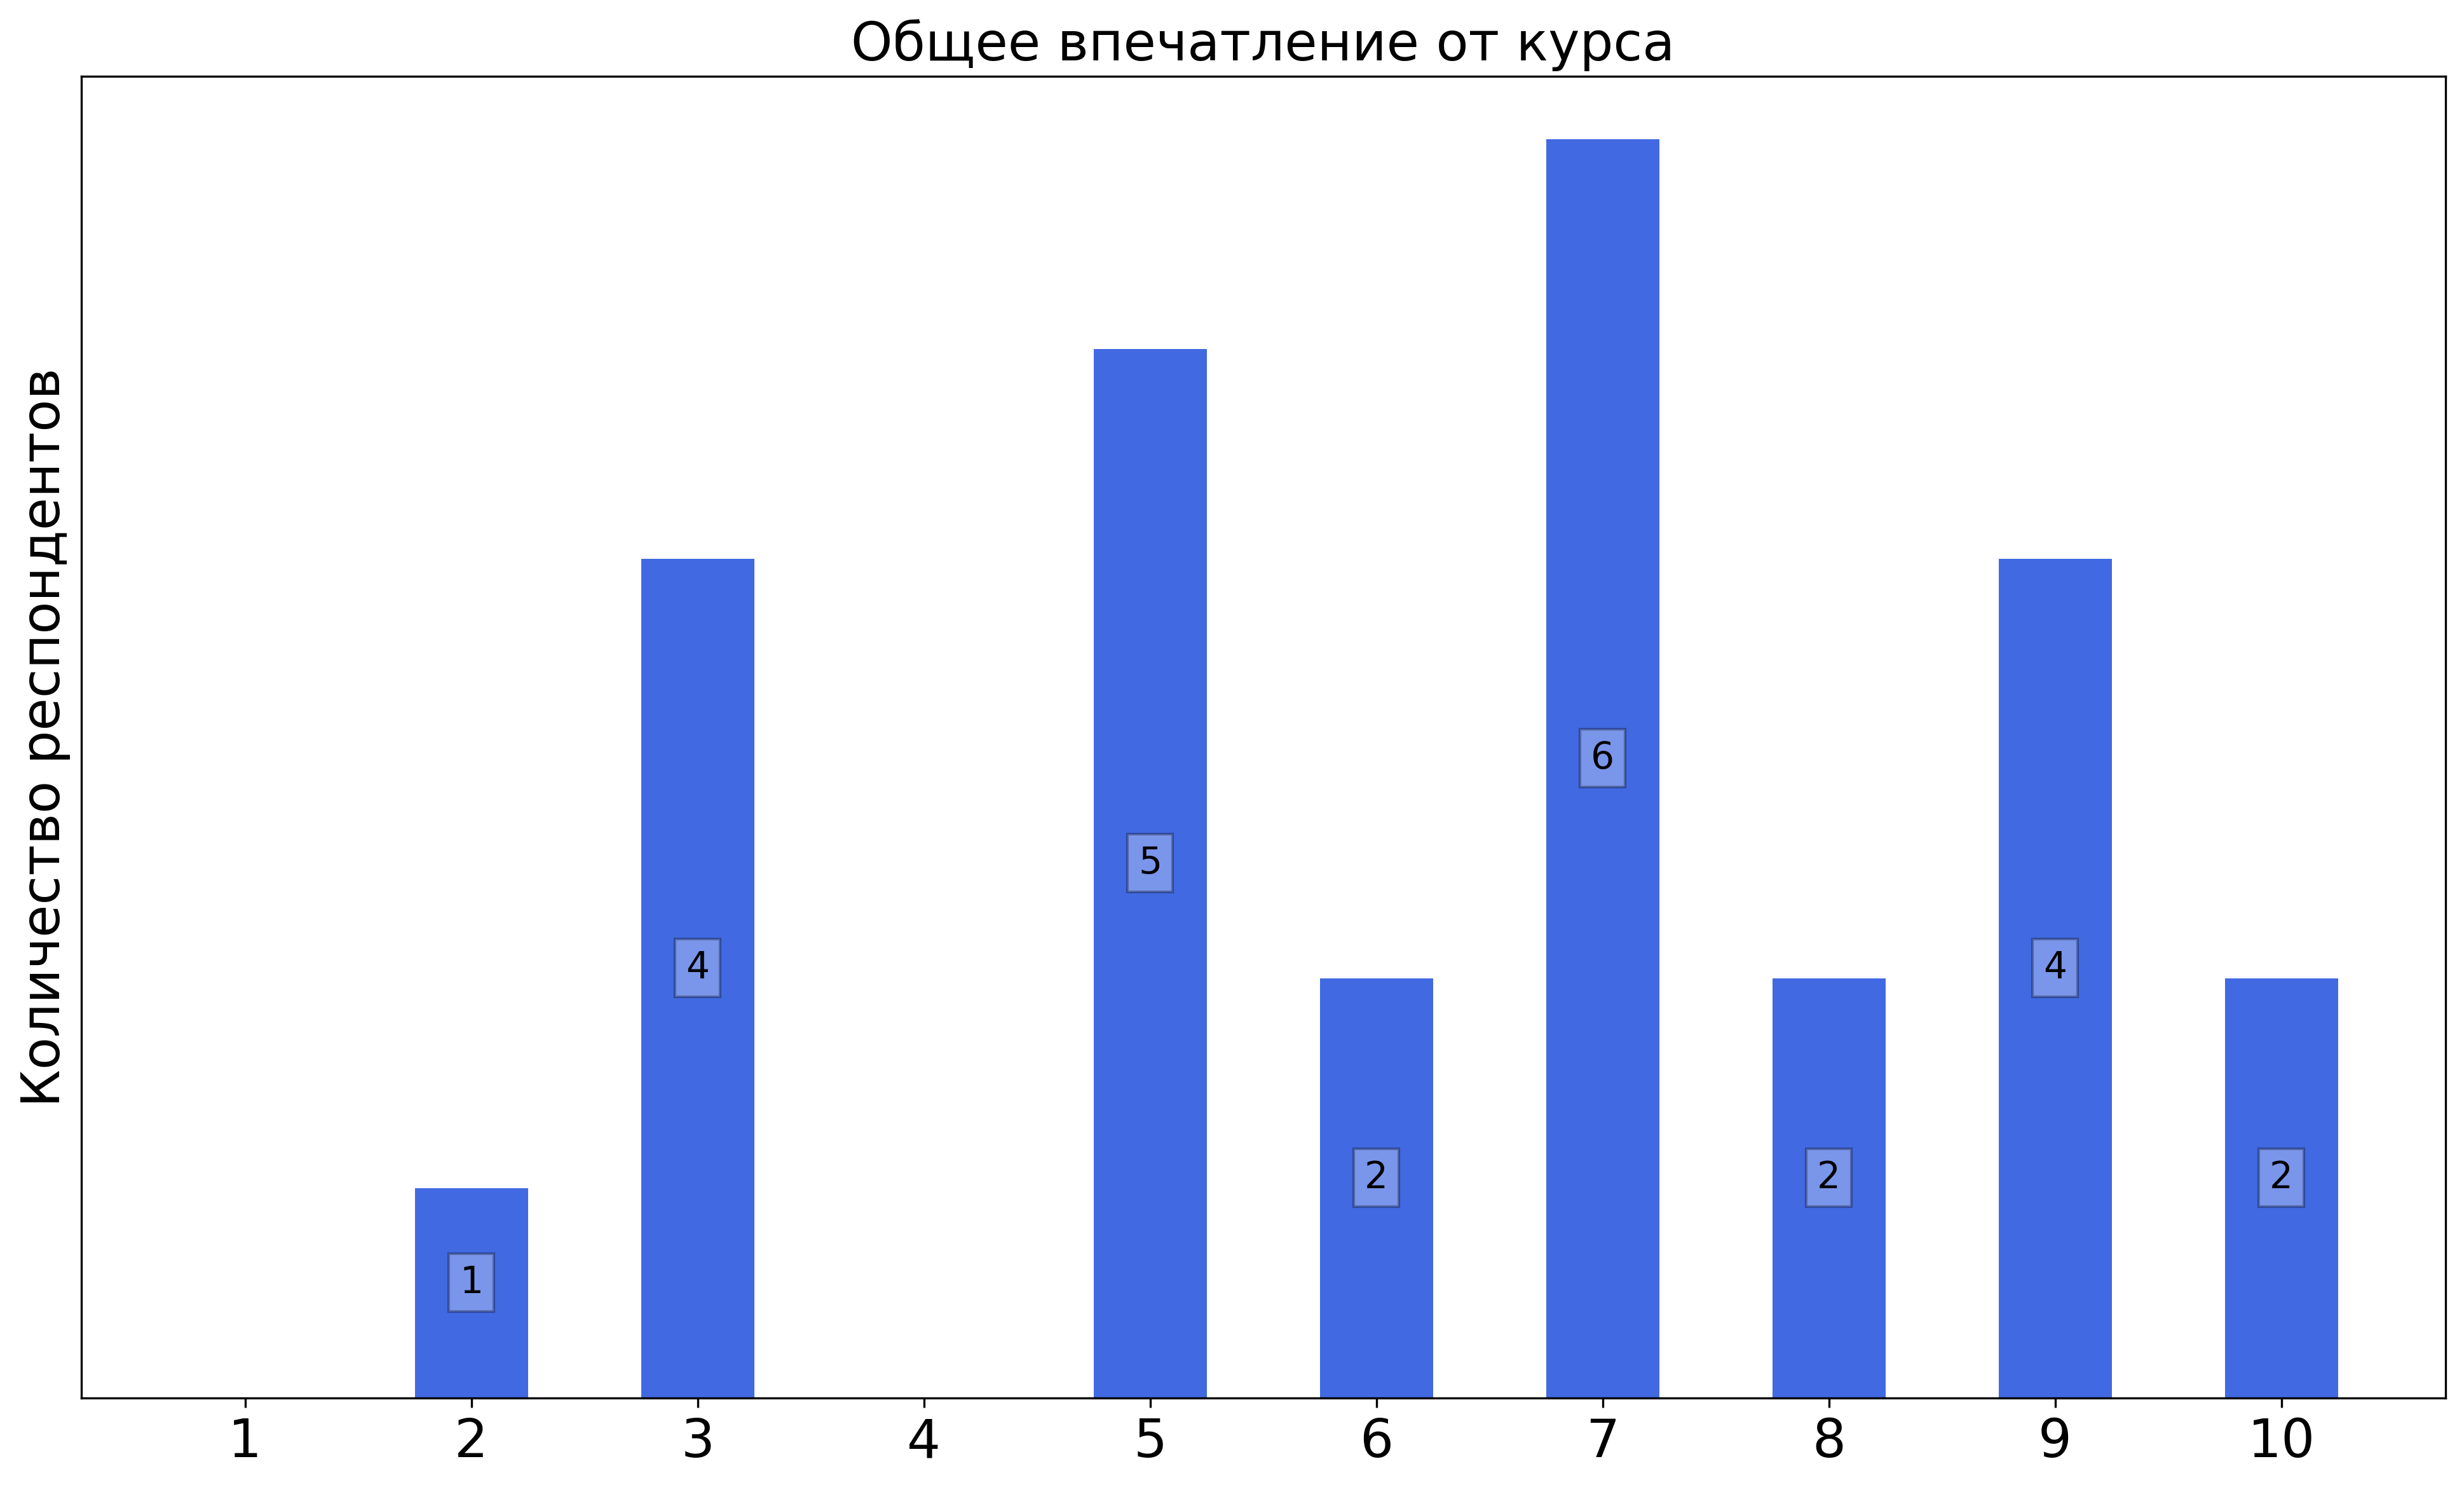
\includegraphics[width=\textwidth]{images/2 course/Компьютерные технологии/general-0.png}
			\end{subfigure}
		\end{figure}

	\subsubsection{Материалы, использумые респондентами при изучении курса}

		\begin{figure}[H]
			\centering
			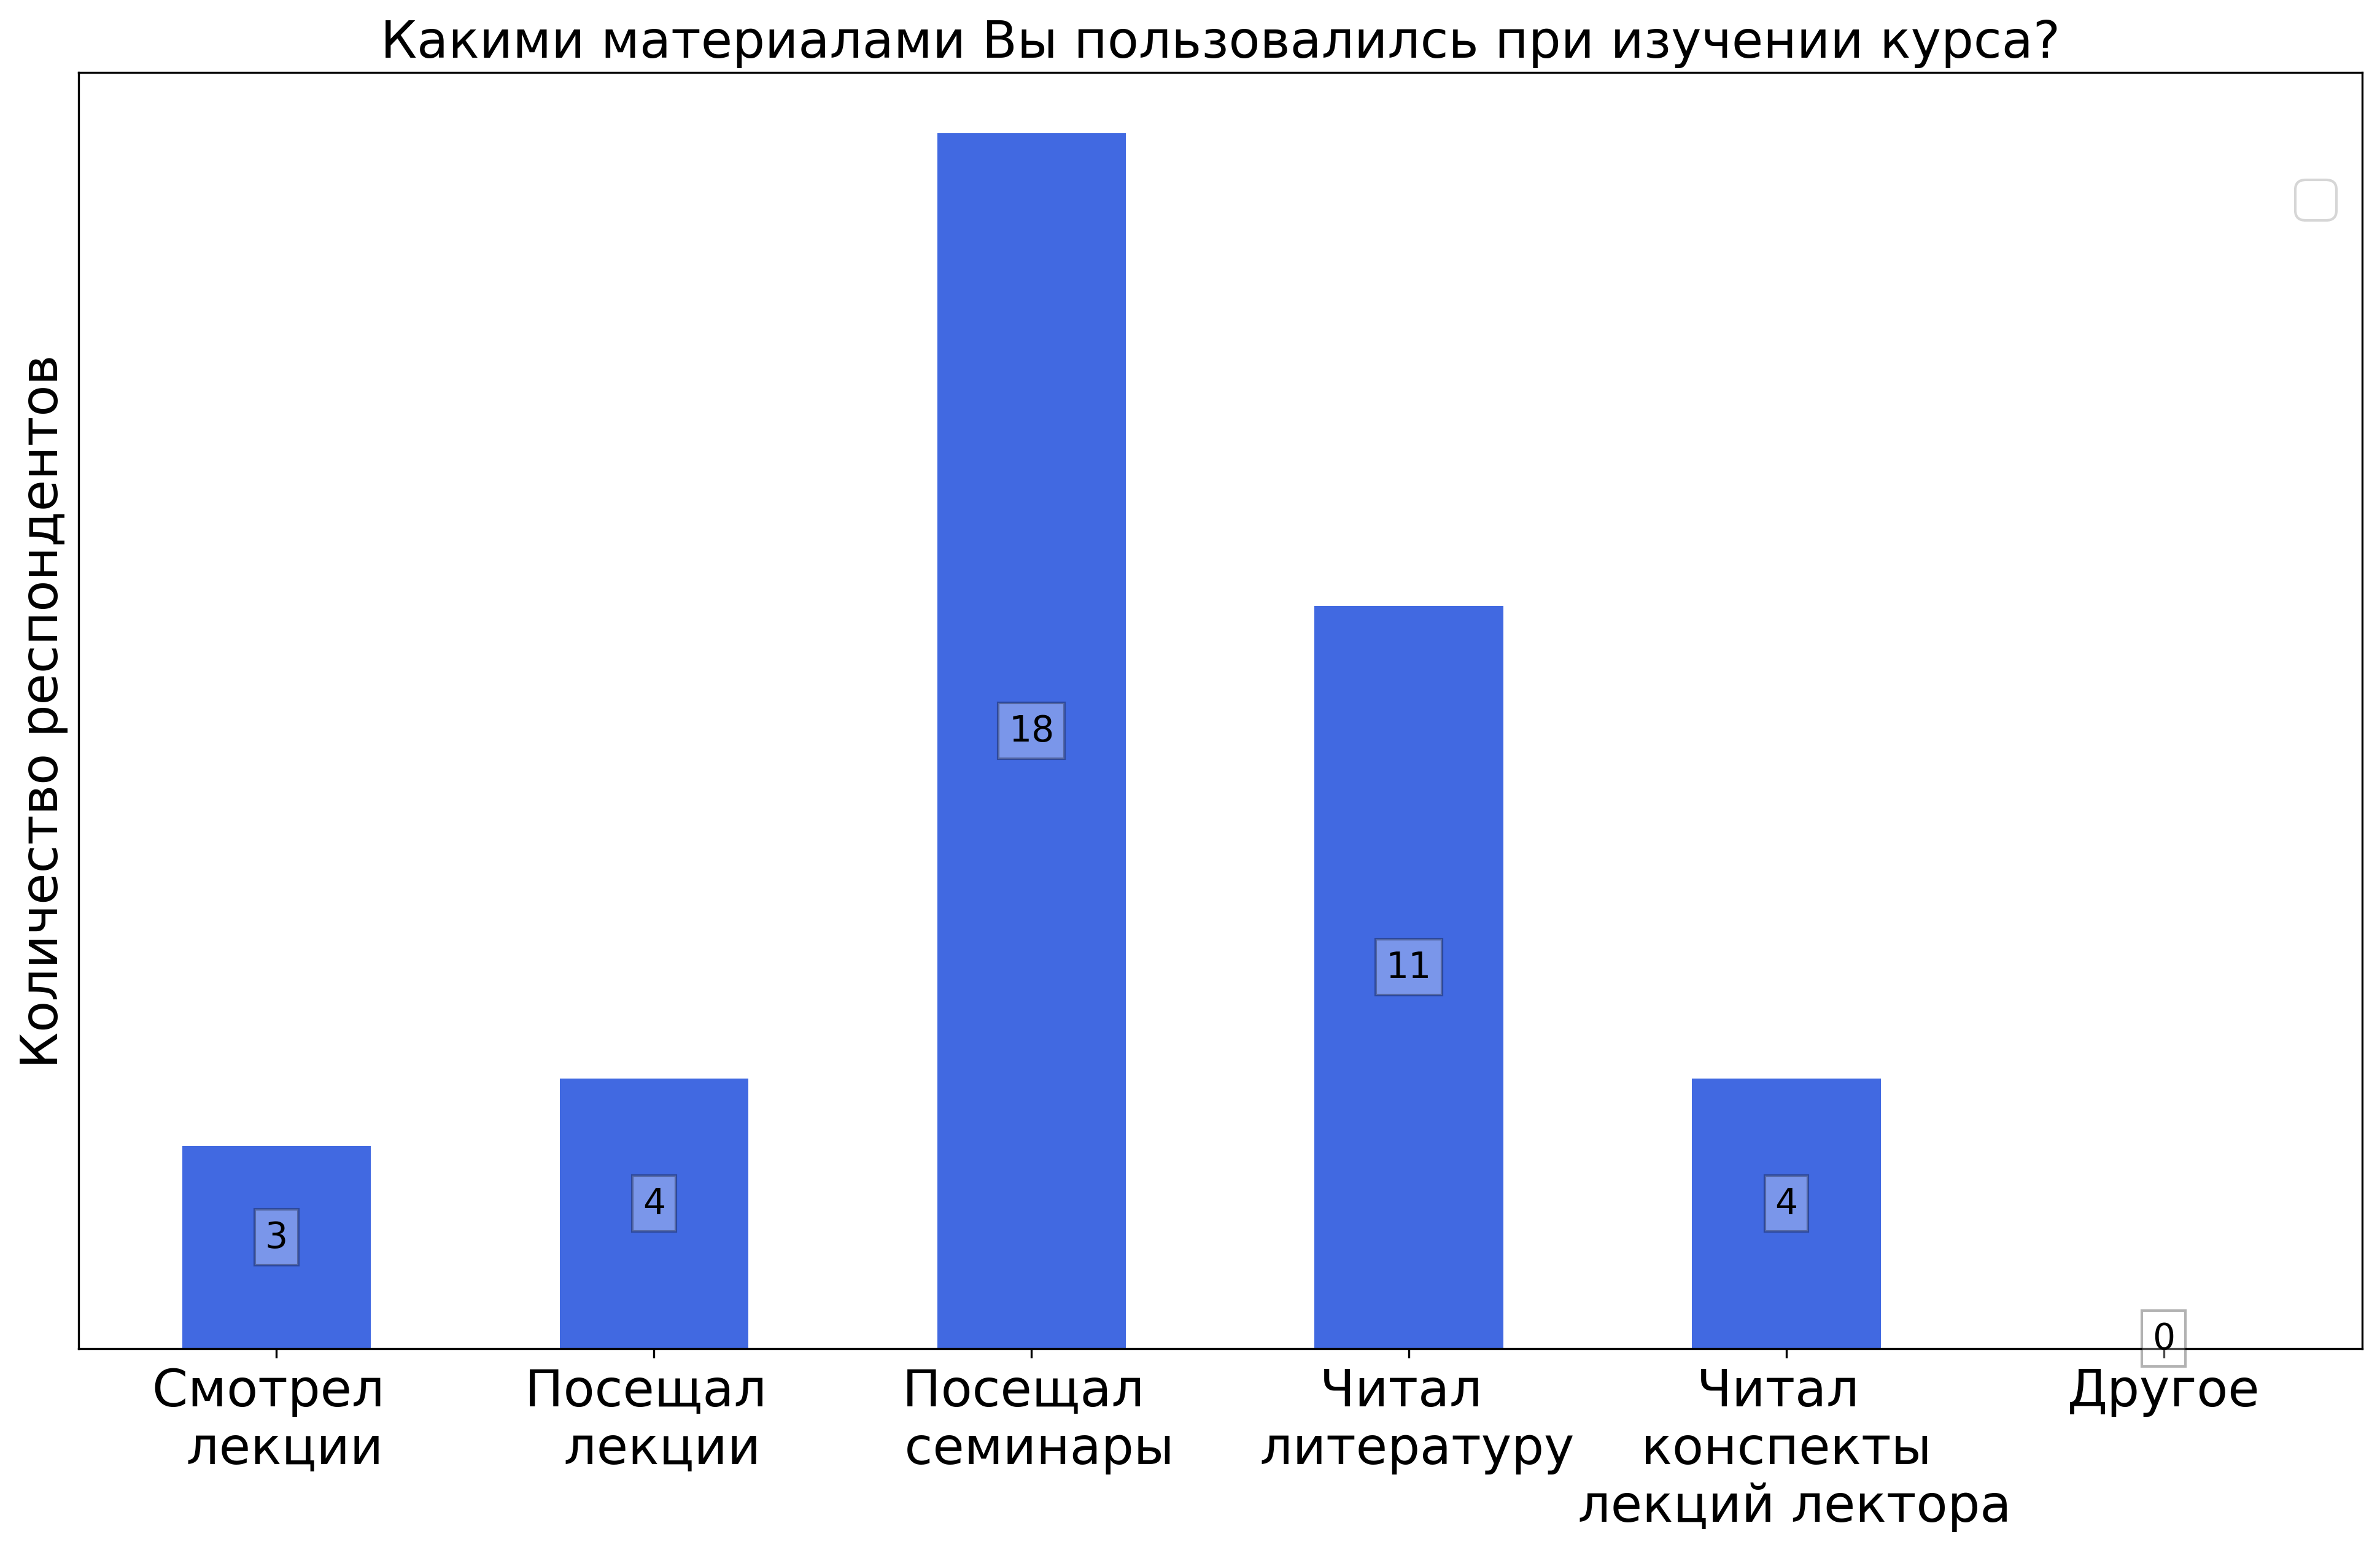
\includegraphics[width = 0.45\textwidth]{images/2 course/Компьютерные технологии/materials.png}
		\end{figure}

	\subsubsection{Отзыв студентов о лекциях. Лектор: Ефанов Н.Н.}

		\begin{figure}[H]
			\centering
            \begin{subfigure}[b]{0.45\textwidth}
				\centering
				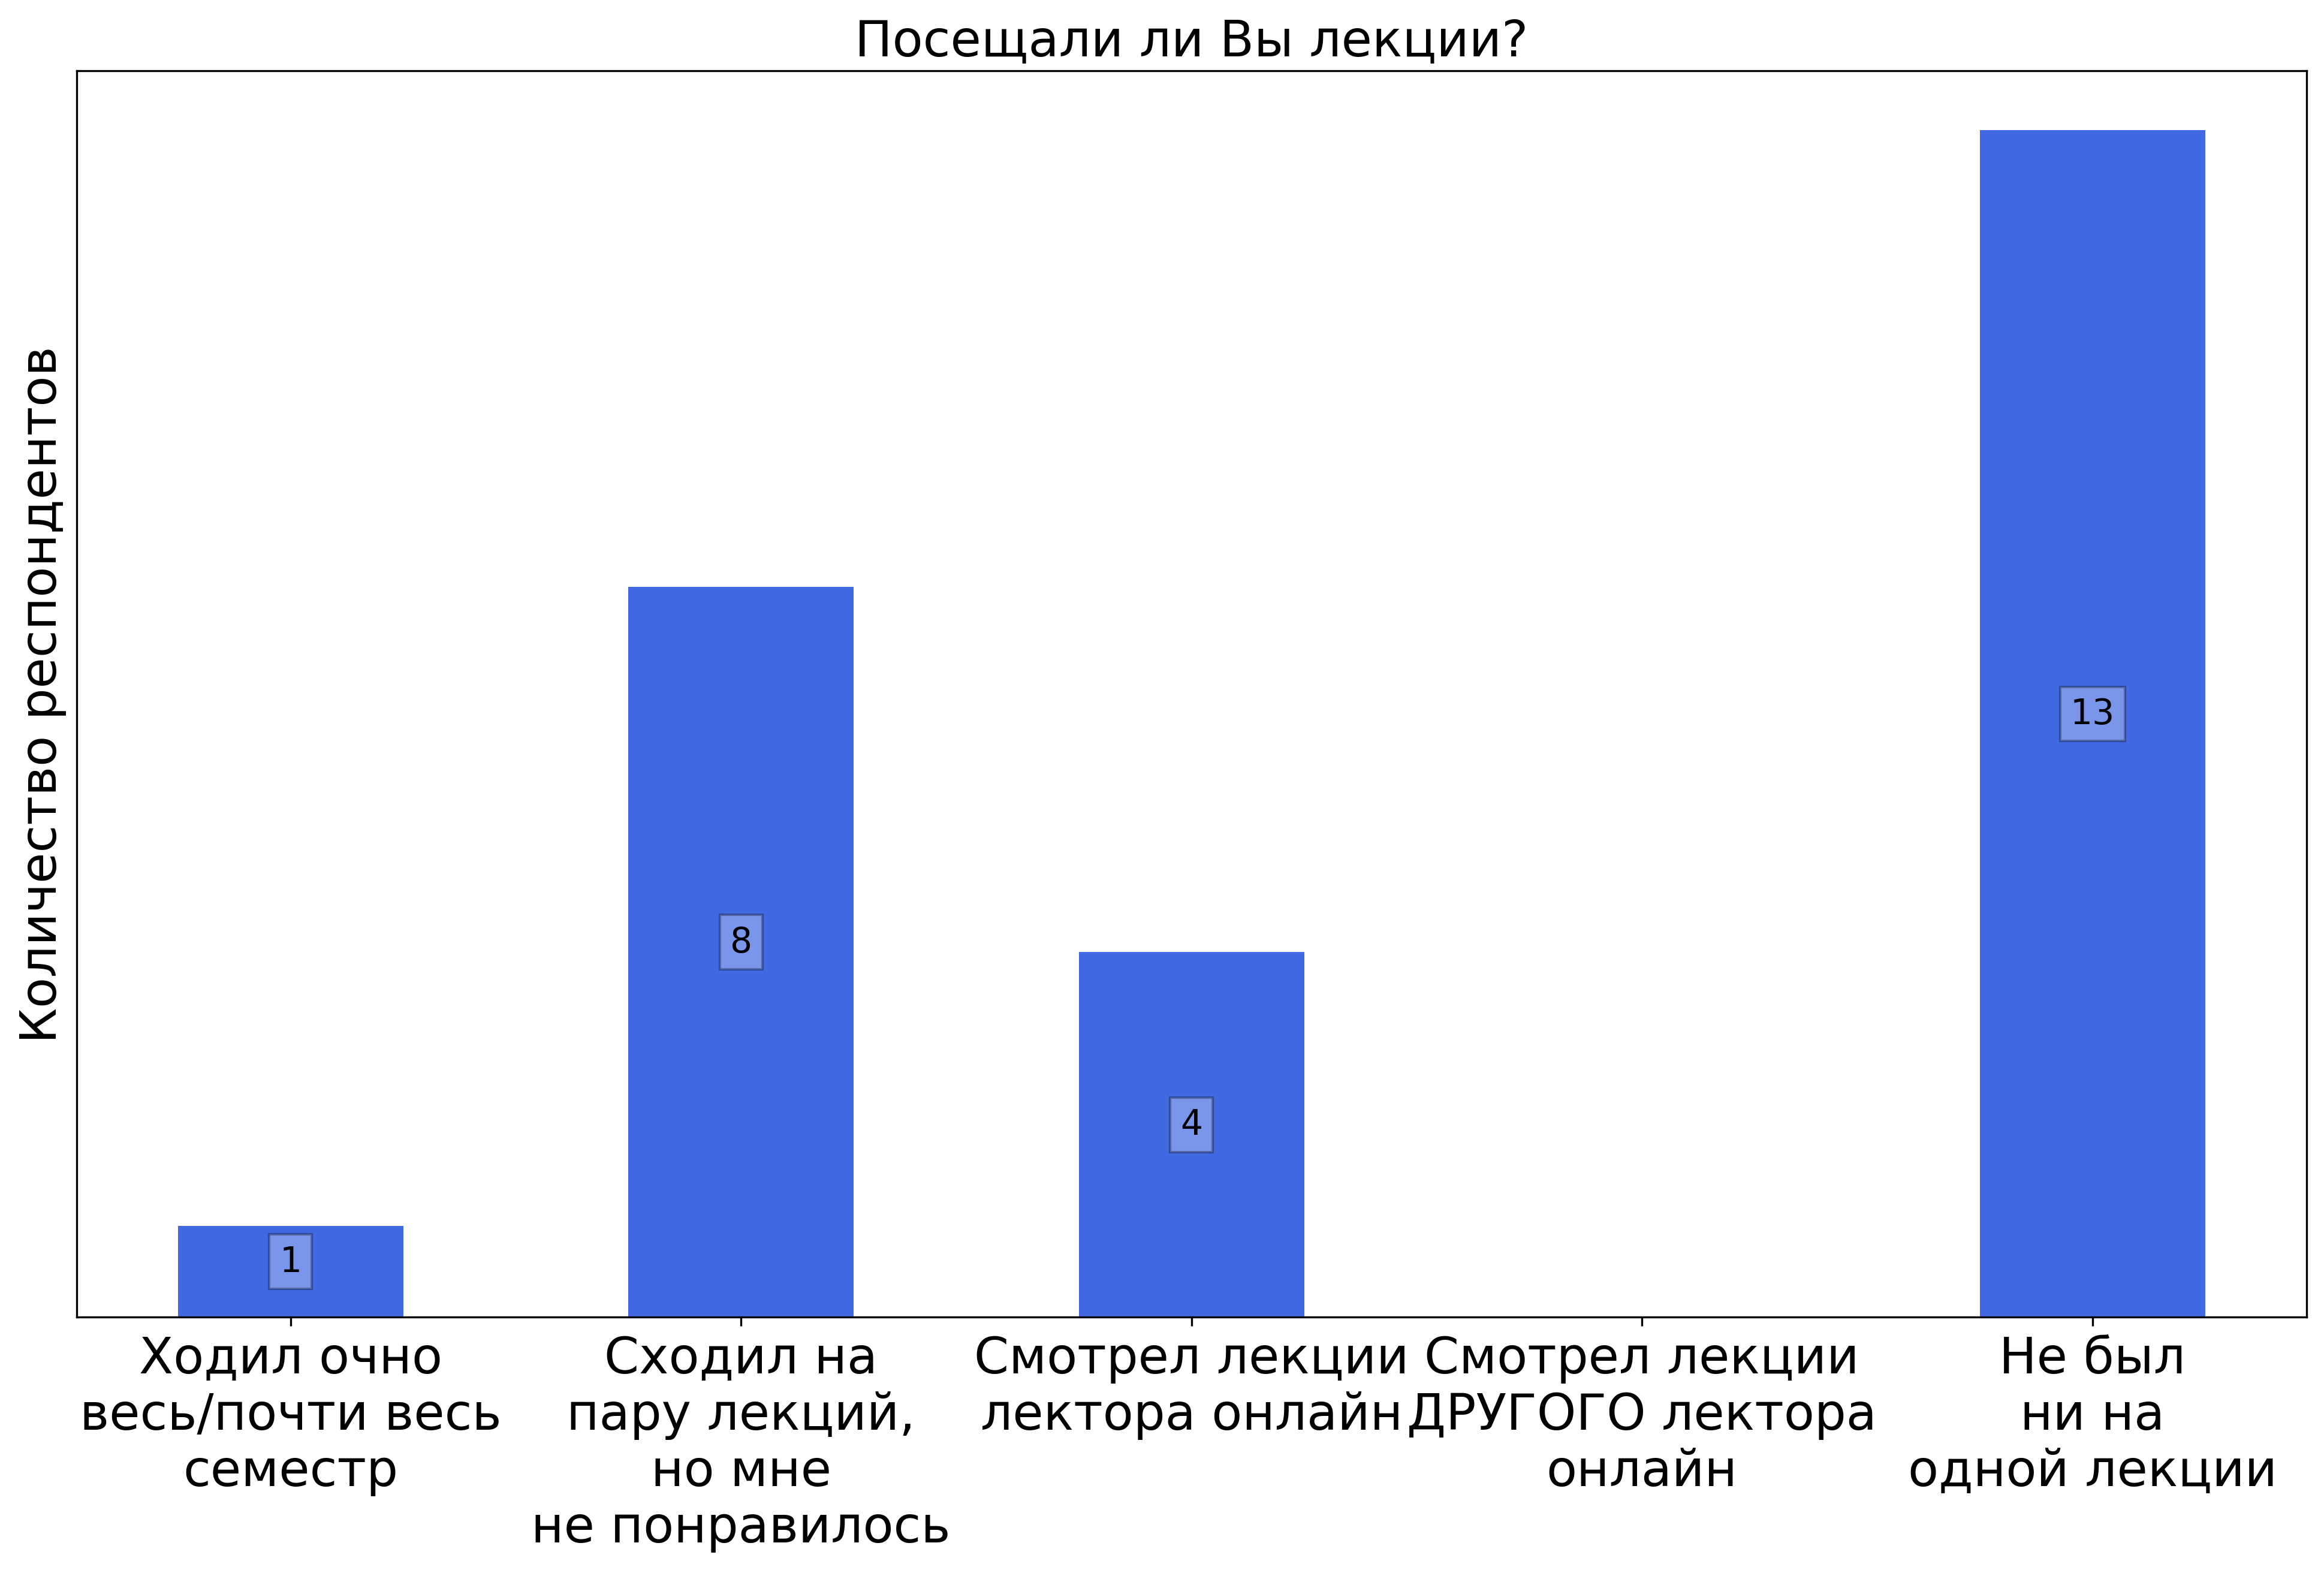
\includegraphics[width=\textwidth]{images/2 course/Компьютерные технологии/lecturer-questions-Ефанов Н.Н.-0.png}
			\end{subfigure}
			\begin{subfigure}[b]{0.45\textwidth}
				\centering
				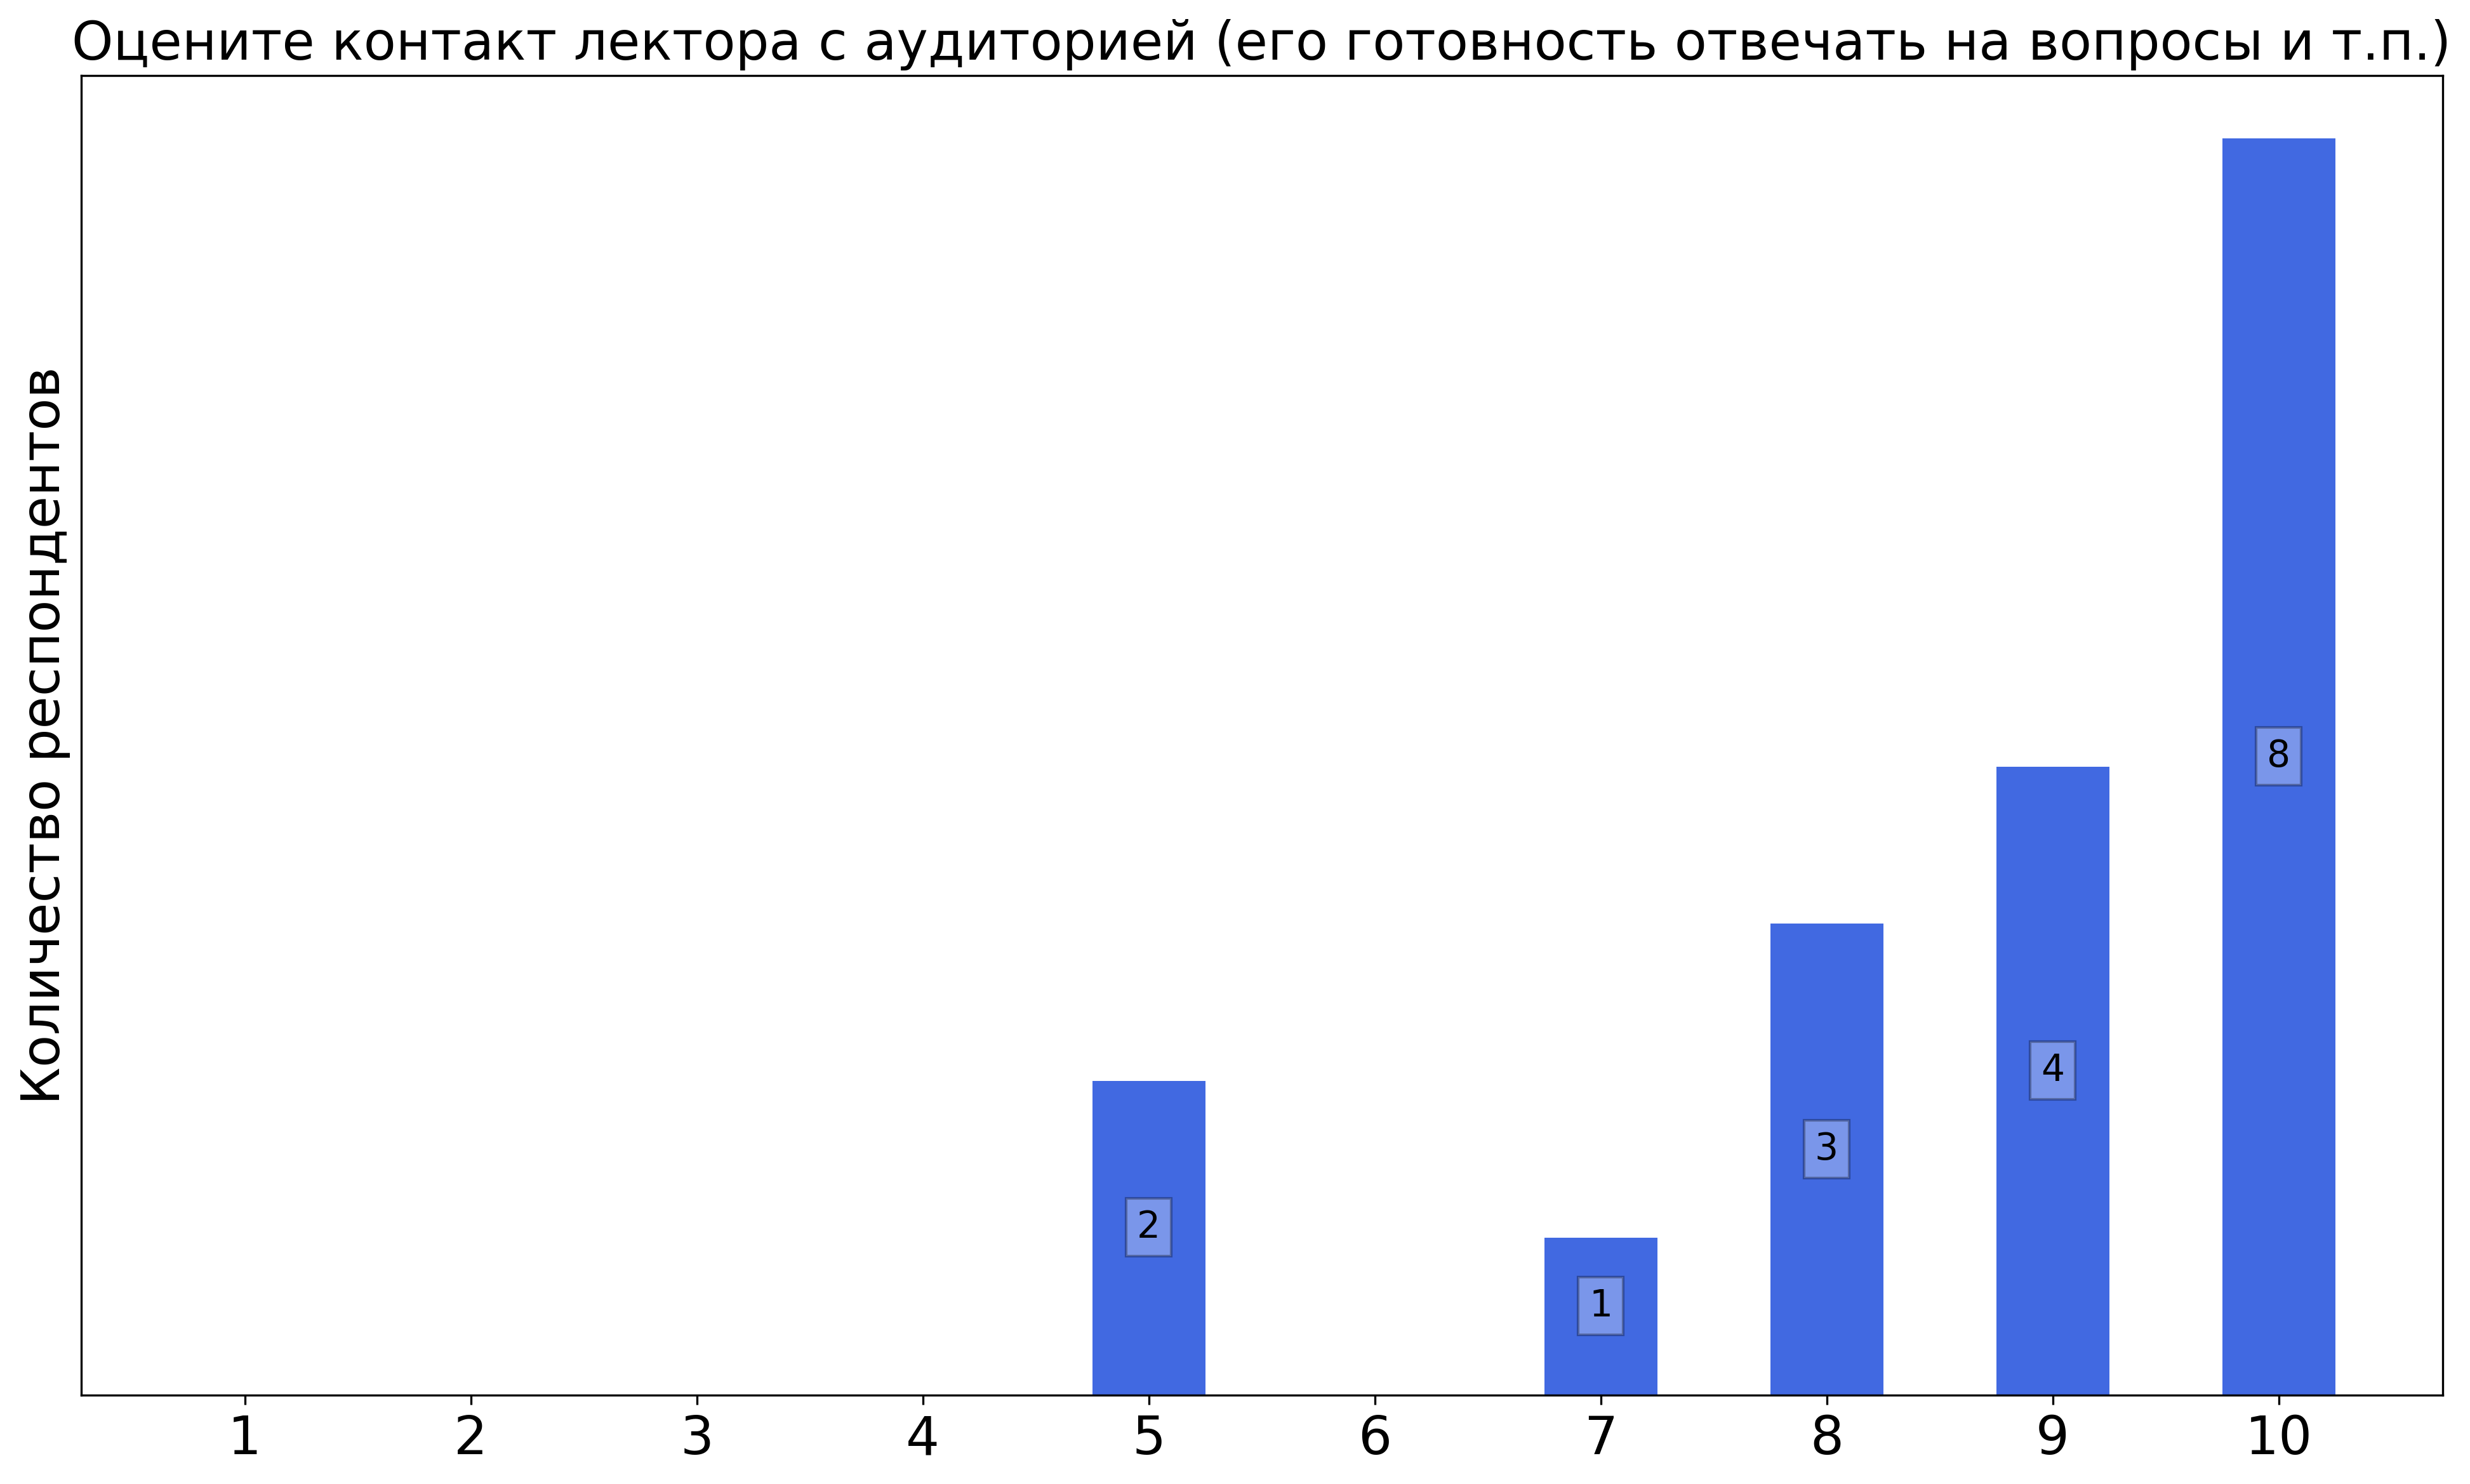
\includegraphics[width=\textwidth]{images/2 course/Компьютерные технологии/lecturer-marks-Ефанов Н.Н.-0.png}
			\end{subfigure}
			\begin{subfigure}[b]{0.45\textwidth}
				\centering
				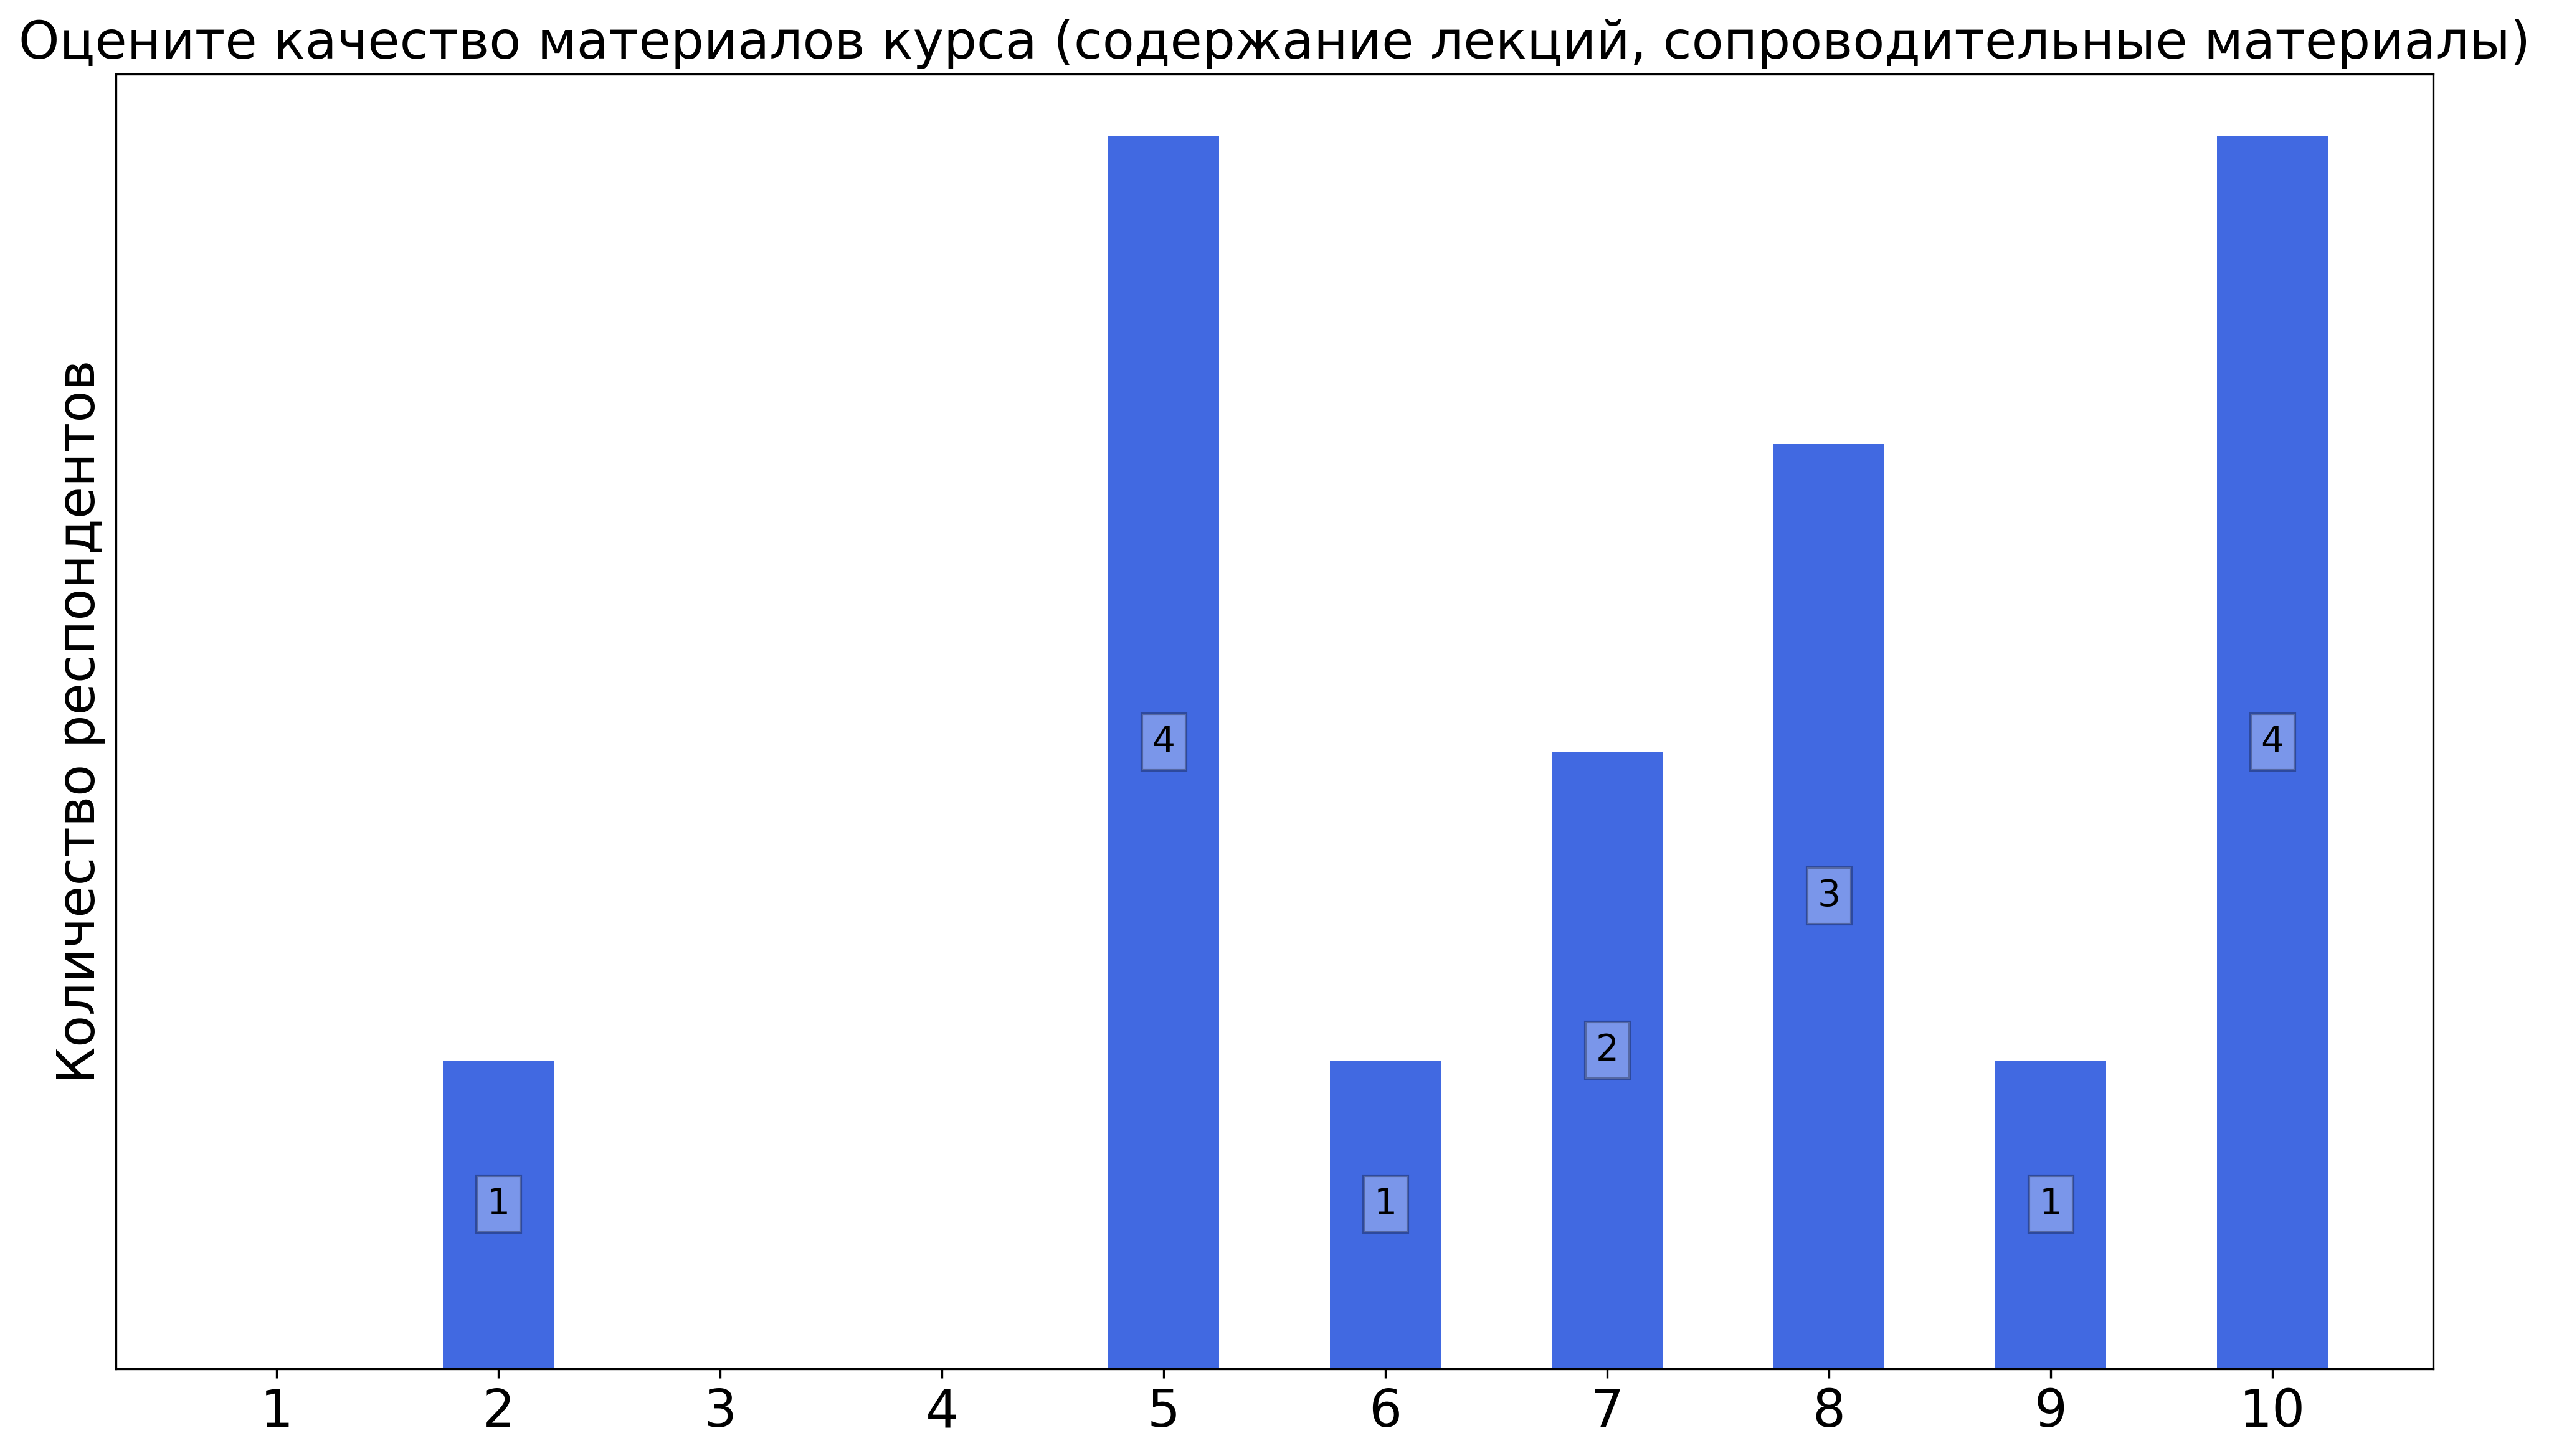
\includegraphics[width=\textwidth]{images/2 course/Компьютерные технологии/lecturer-marks-Ефанов Н.Н.-1.png}
			\end{subfigure}
			\begin{subfigure}[b]{0.45\textwidth}
				\centering
				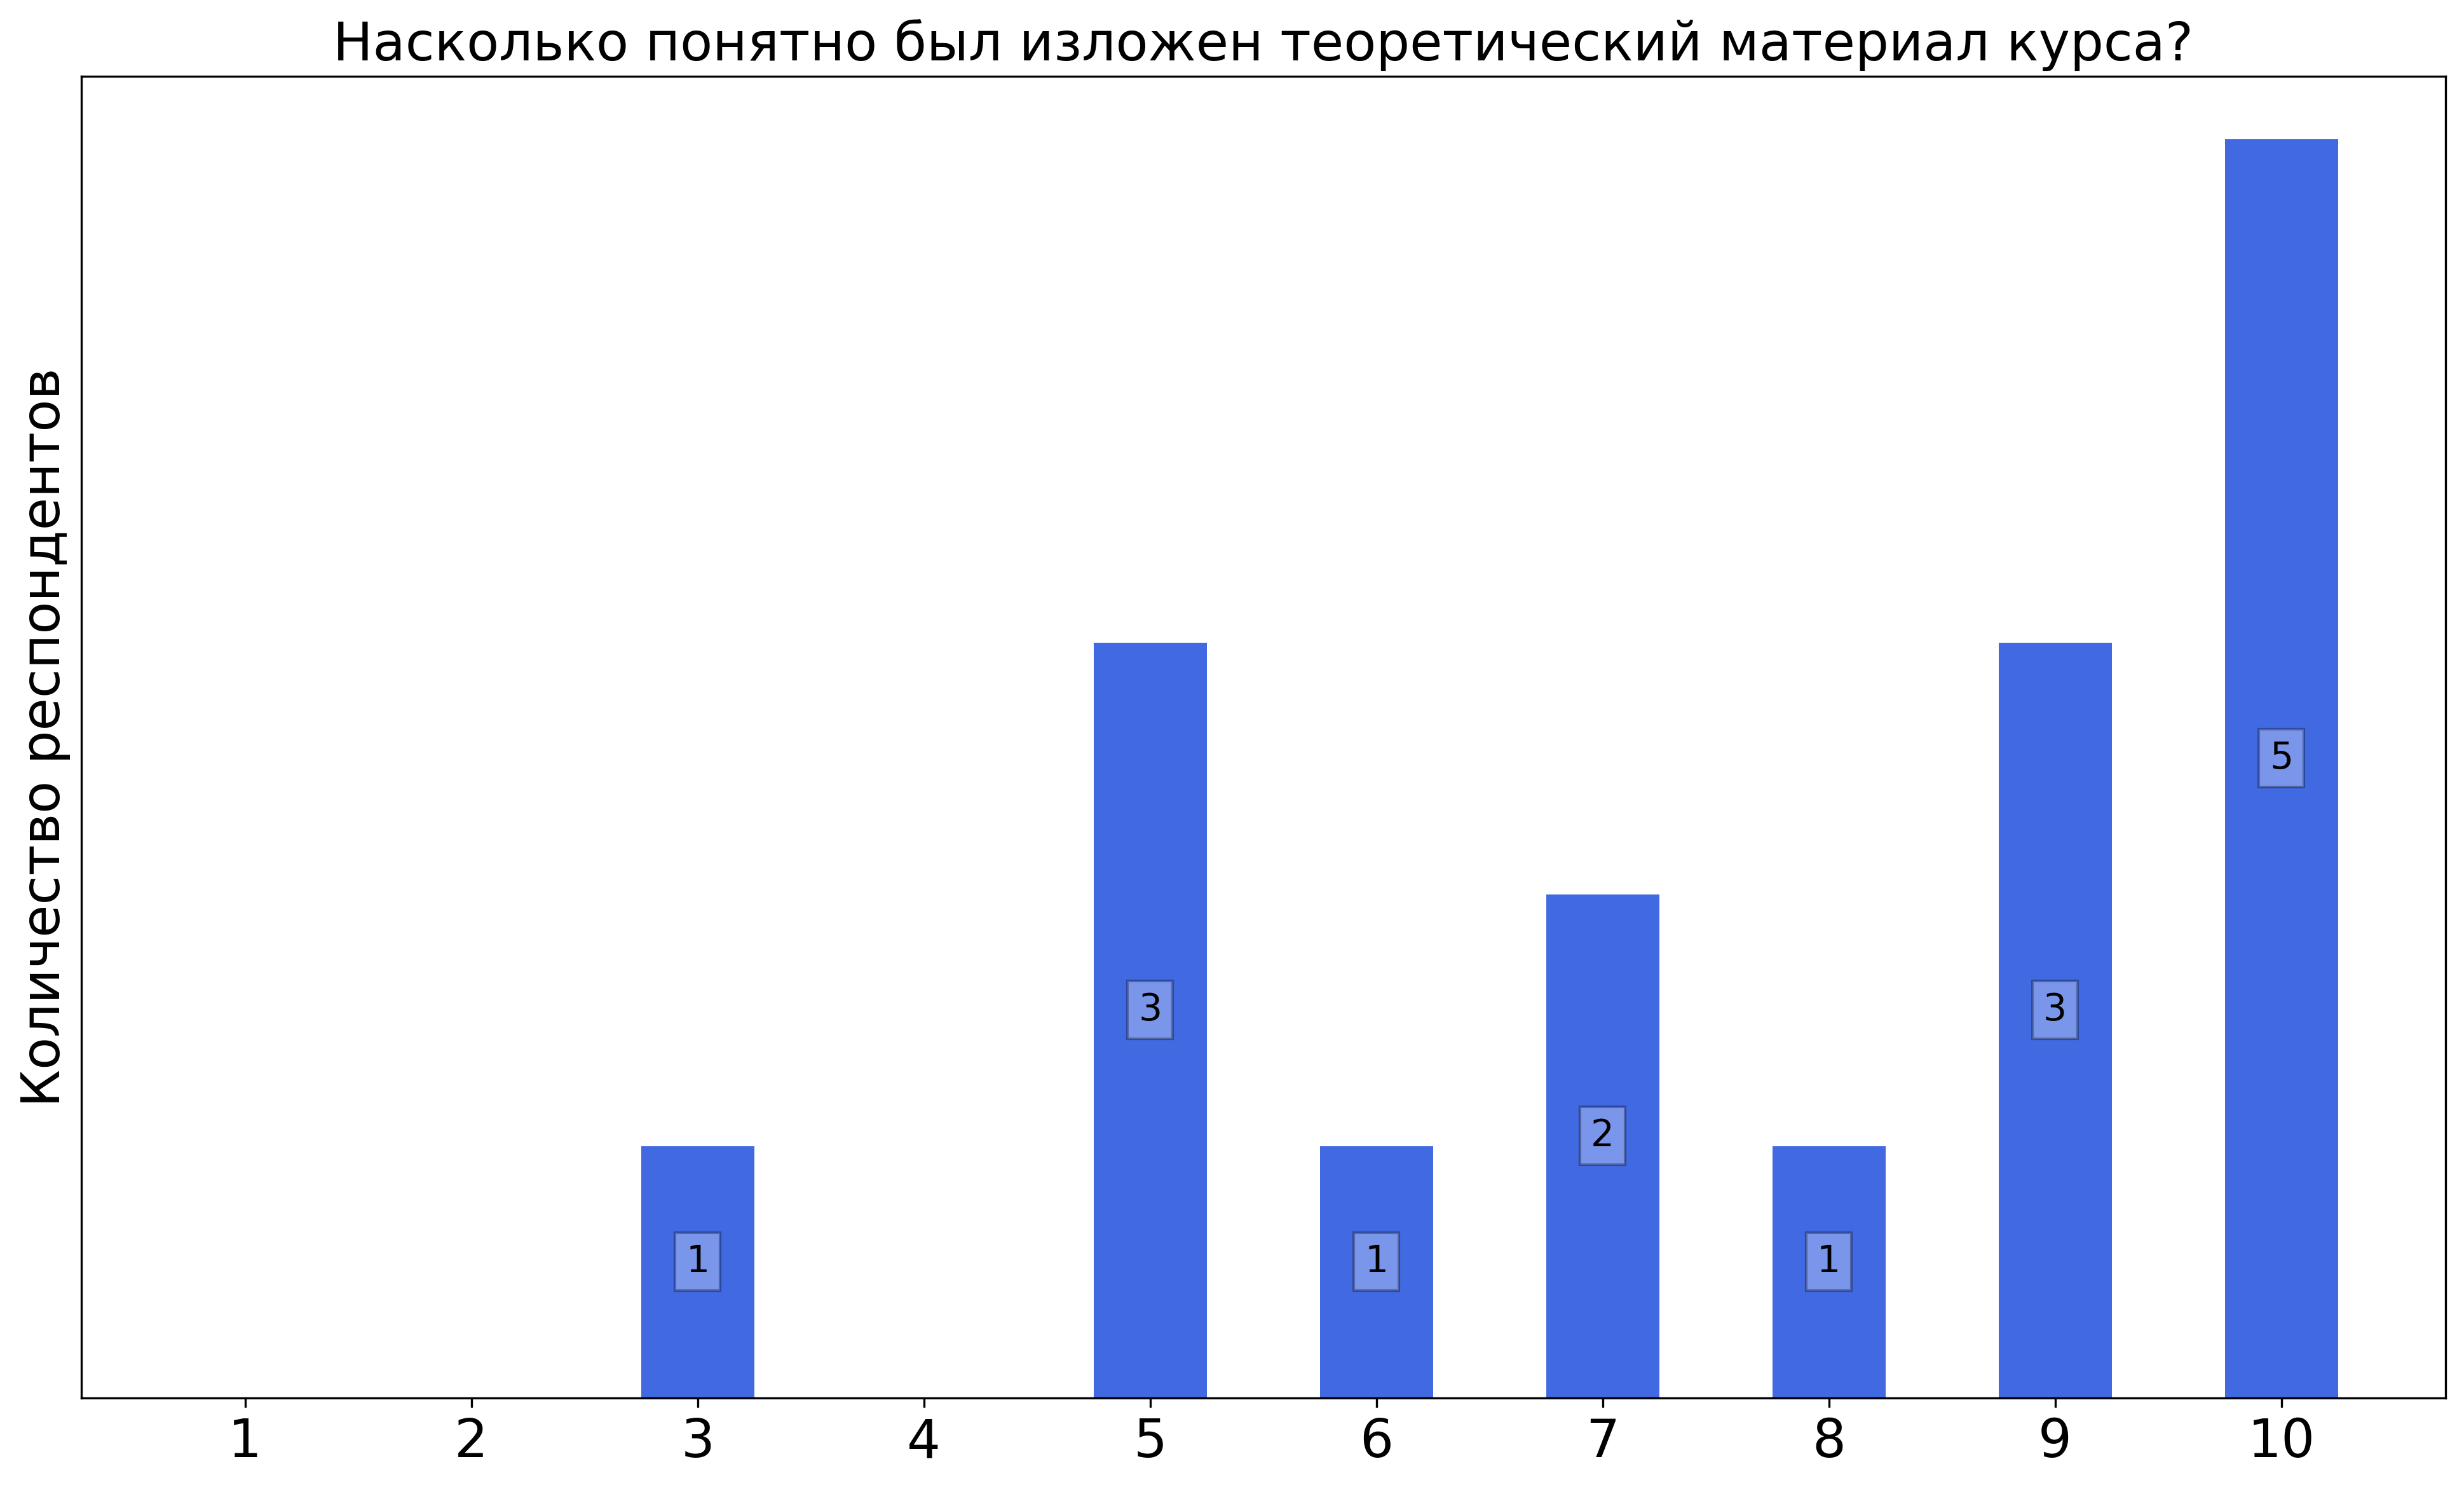
\includegraphics[width=\textwidth]{images/2 course/Компьютерные технологии/lecturer-marks-Ефанов Н.Н.-2.png}
			\end{subfigure}	
			\begin{subfigure}[b]{0.45\textwidth}
				\centering
				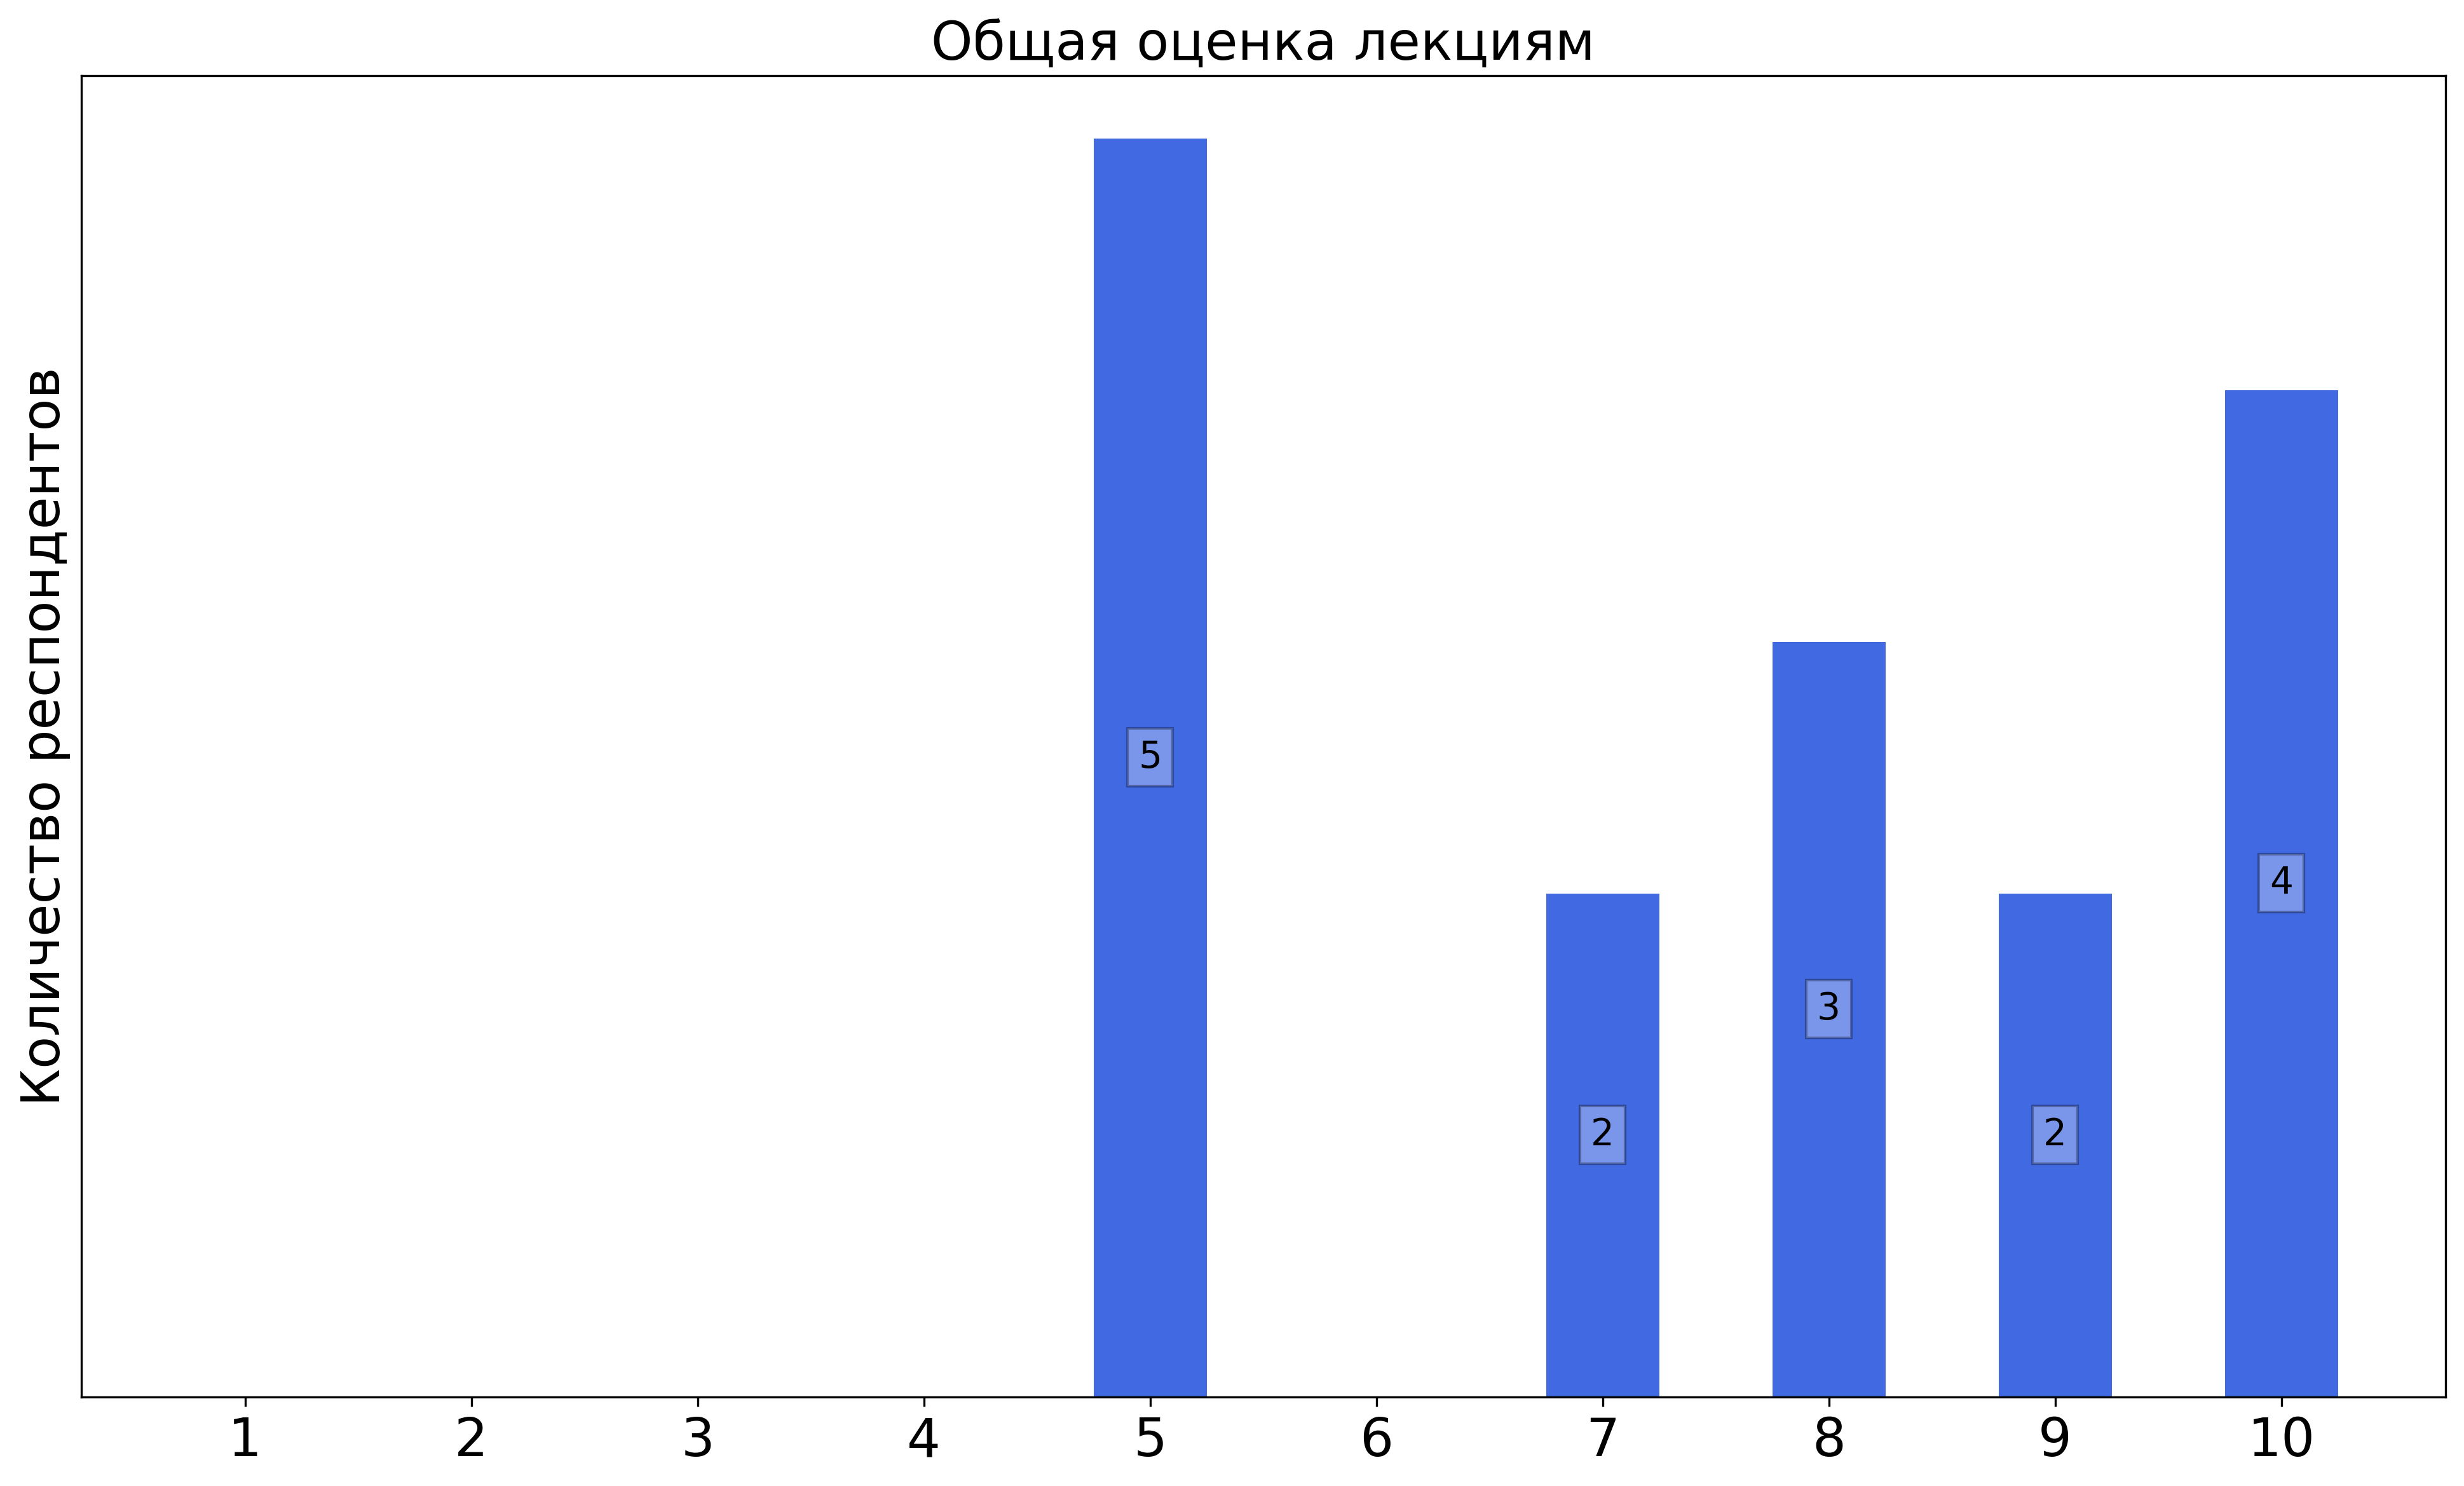
\includegraphics[width=\textwidth]{images/2 course/Компьютерные технологии/lecturer-marks-Ефанов Н.Н.-3.png}
			\end{subfigure}
			\caption{Оценки респондентов о качестве преподавания лекций по курсу <<Компьютерные технологии>>}
		\end{figure}

		\textbf{Комментарии студентов о лекциях\protect\footnote{сохранены оригинальные орфография и пунктуация}}
            \begin{commentbox} 
                грустно что они первой парой  
            \end{commentbox} 
        
            \begin{commentbox} 
                немного путано для понимания, без книг не обойтись
                то, что лекция в 9 утра, тоже не способствует пониманию 
            \end{commentbox} 
        
            \begin{commentbox} 
                Мне было ничего не понятно на лекциях, я даже не знал что спрашивать, хотелось бы больше пояснений и «разжевываний» каждой темы 
            \end{commentbox} 
    
    
    \subsubsection{Отзыв студентов о семинарах. Семинарист: Гутник С.А.}
		\begin{figure}[H]
			\centering
			\begin{subfigure}[b]{0.45\textwidth}
				\centering
				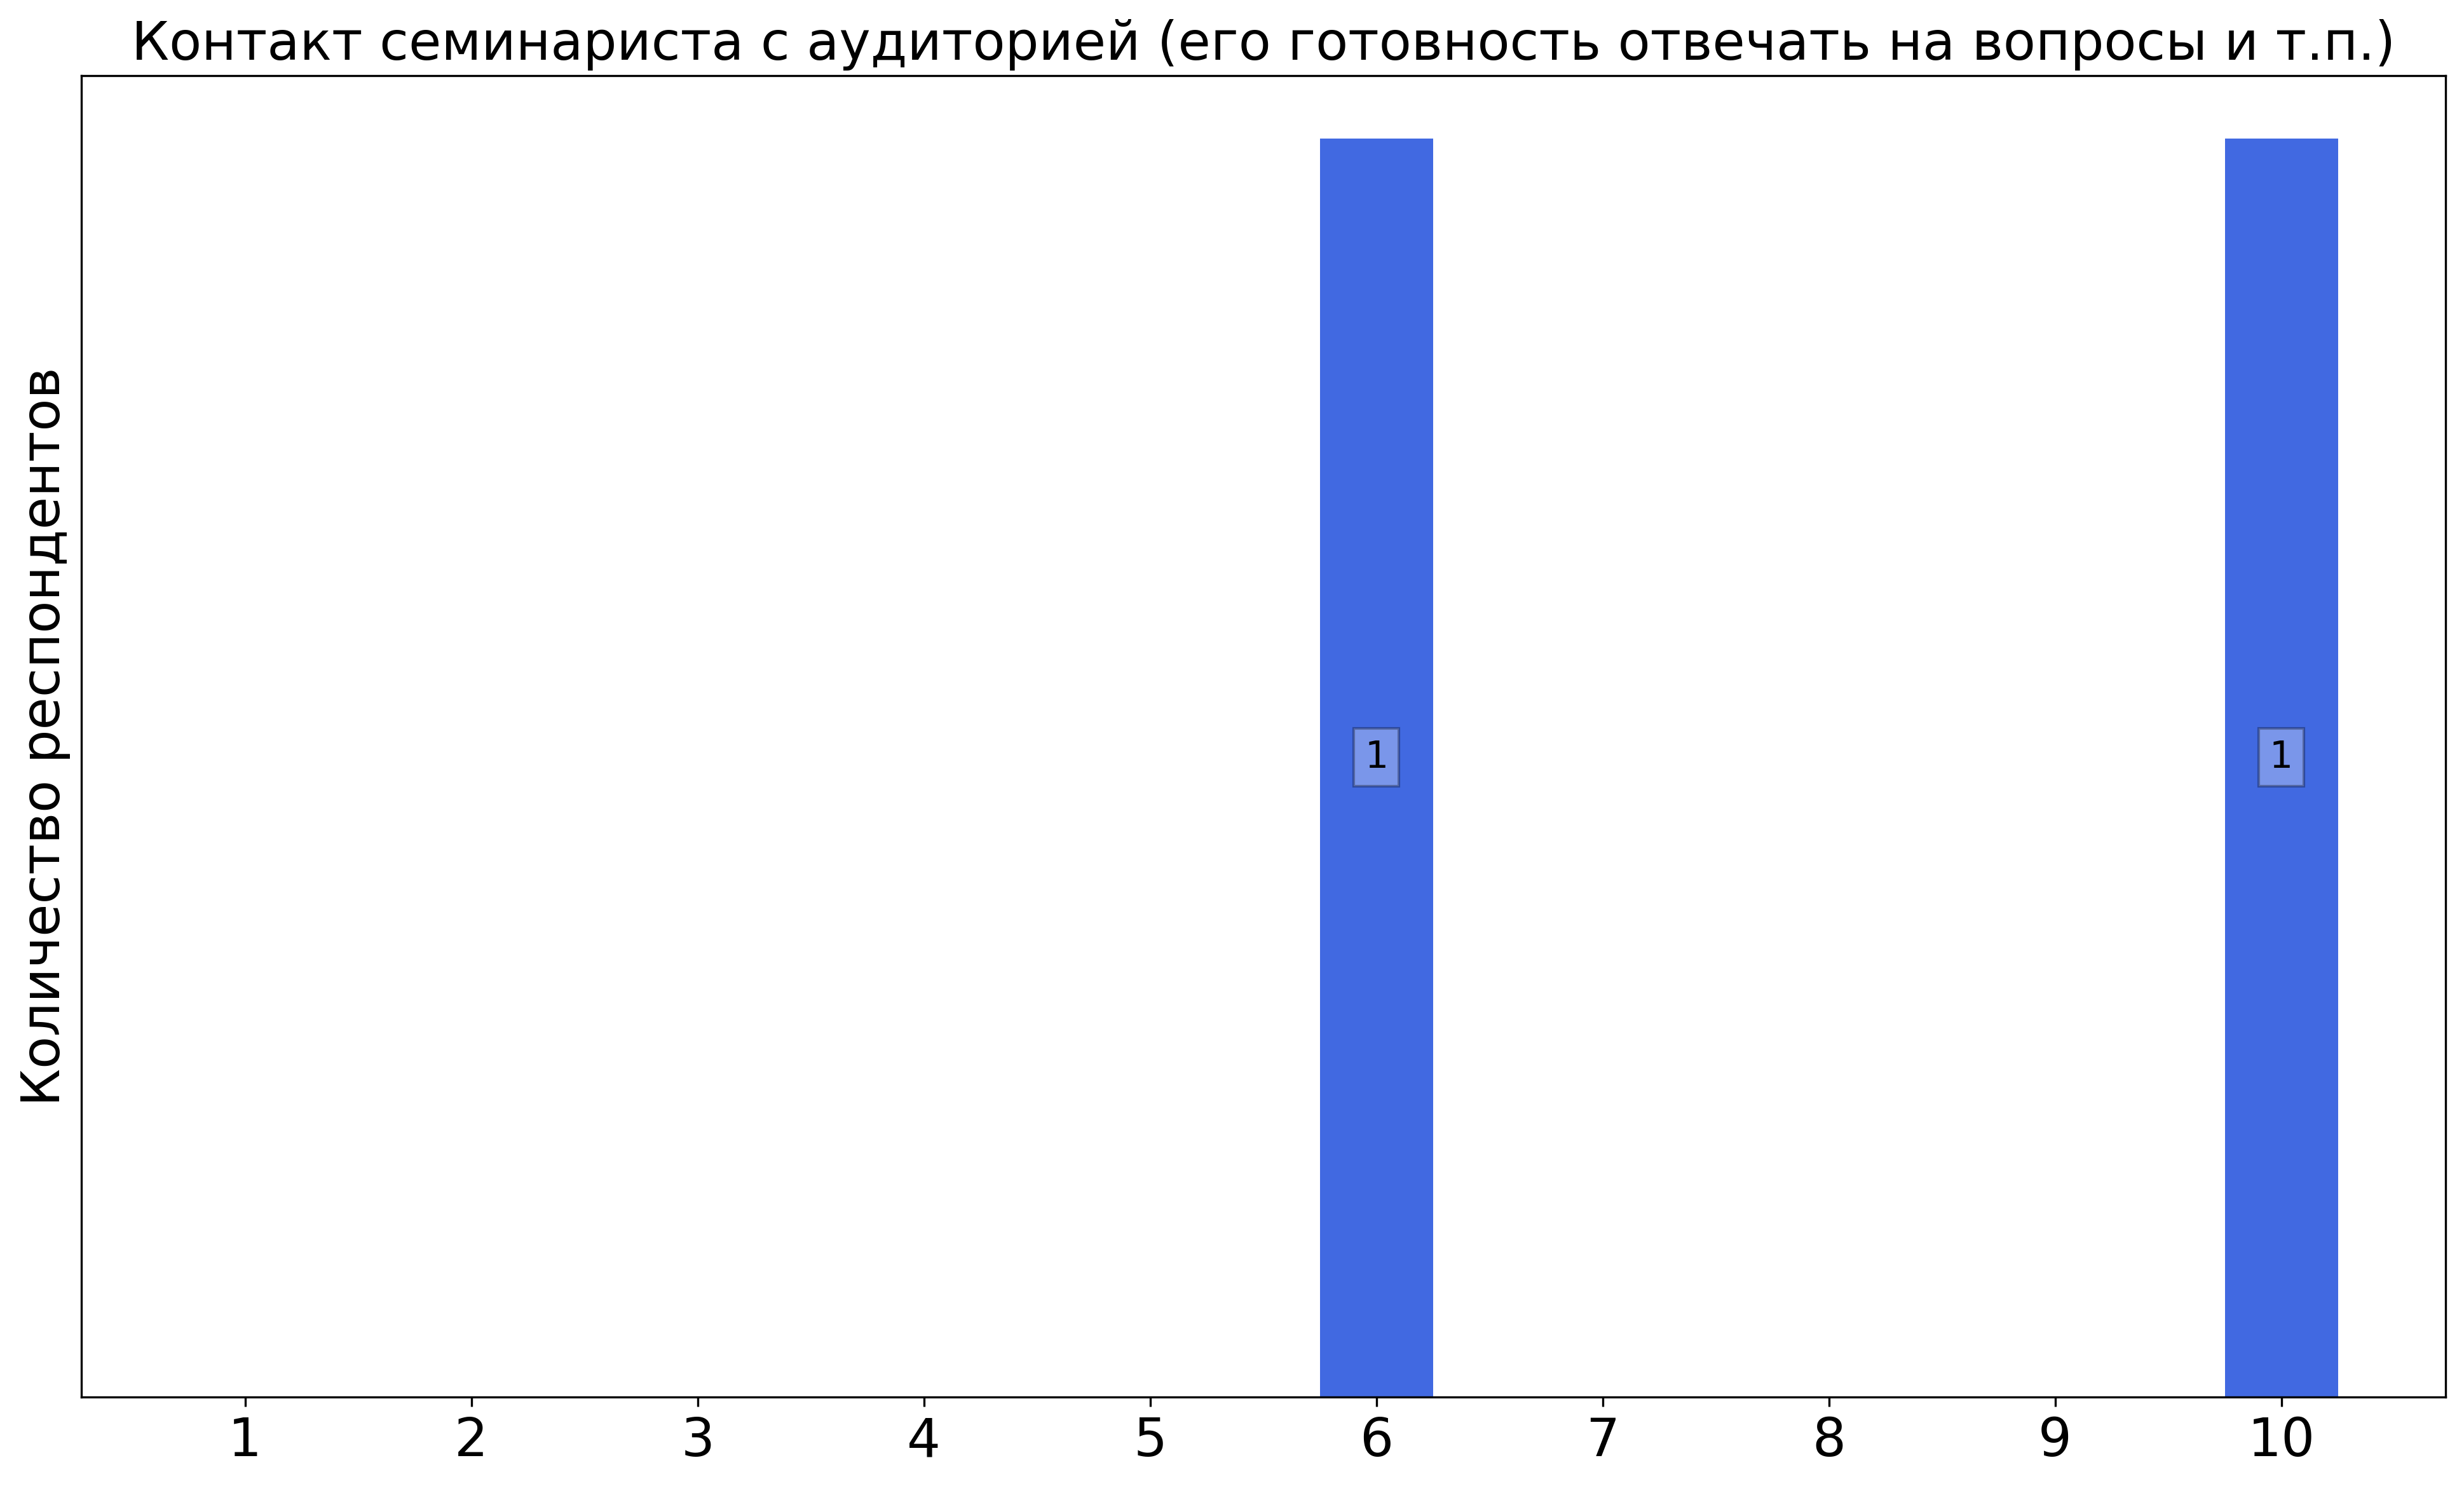
\includegraphics[width=\textwidth]{images/2 course/Компьютерные технологии/seminarists-marks-Гутник С.А.-0.png}
			\end{subfigure}
			\begin{subfigure}[b]{0.45\textwidth}
				\centering
				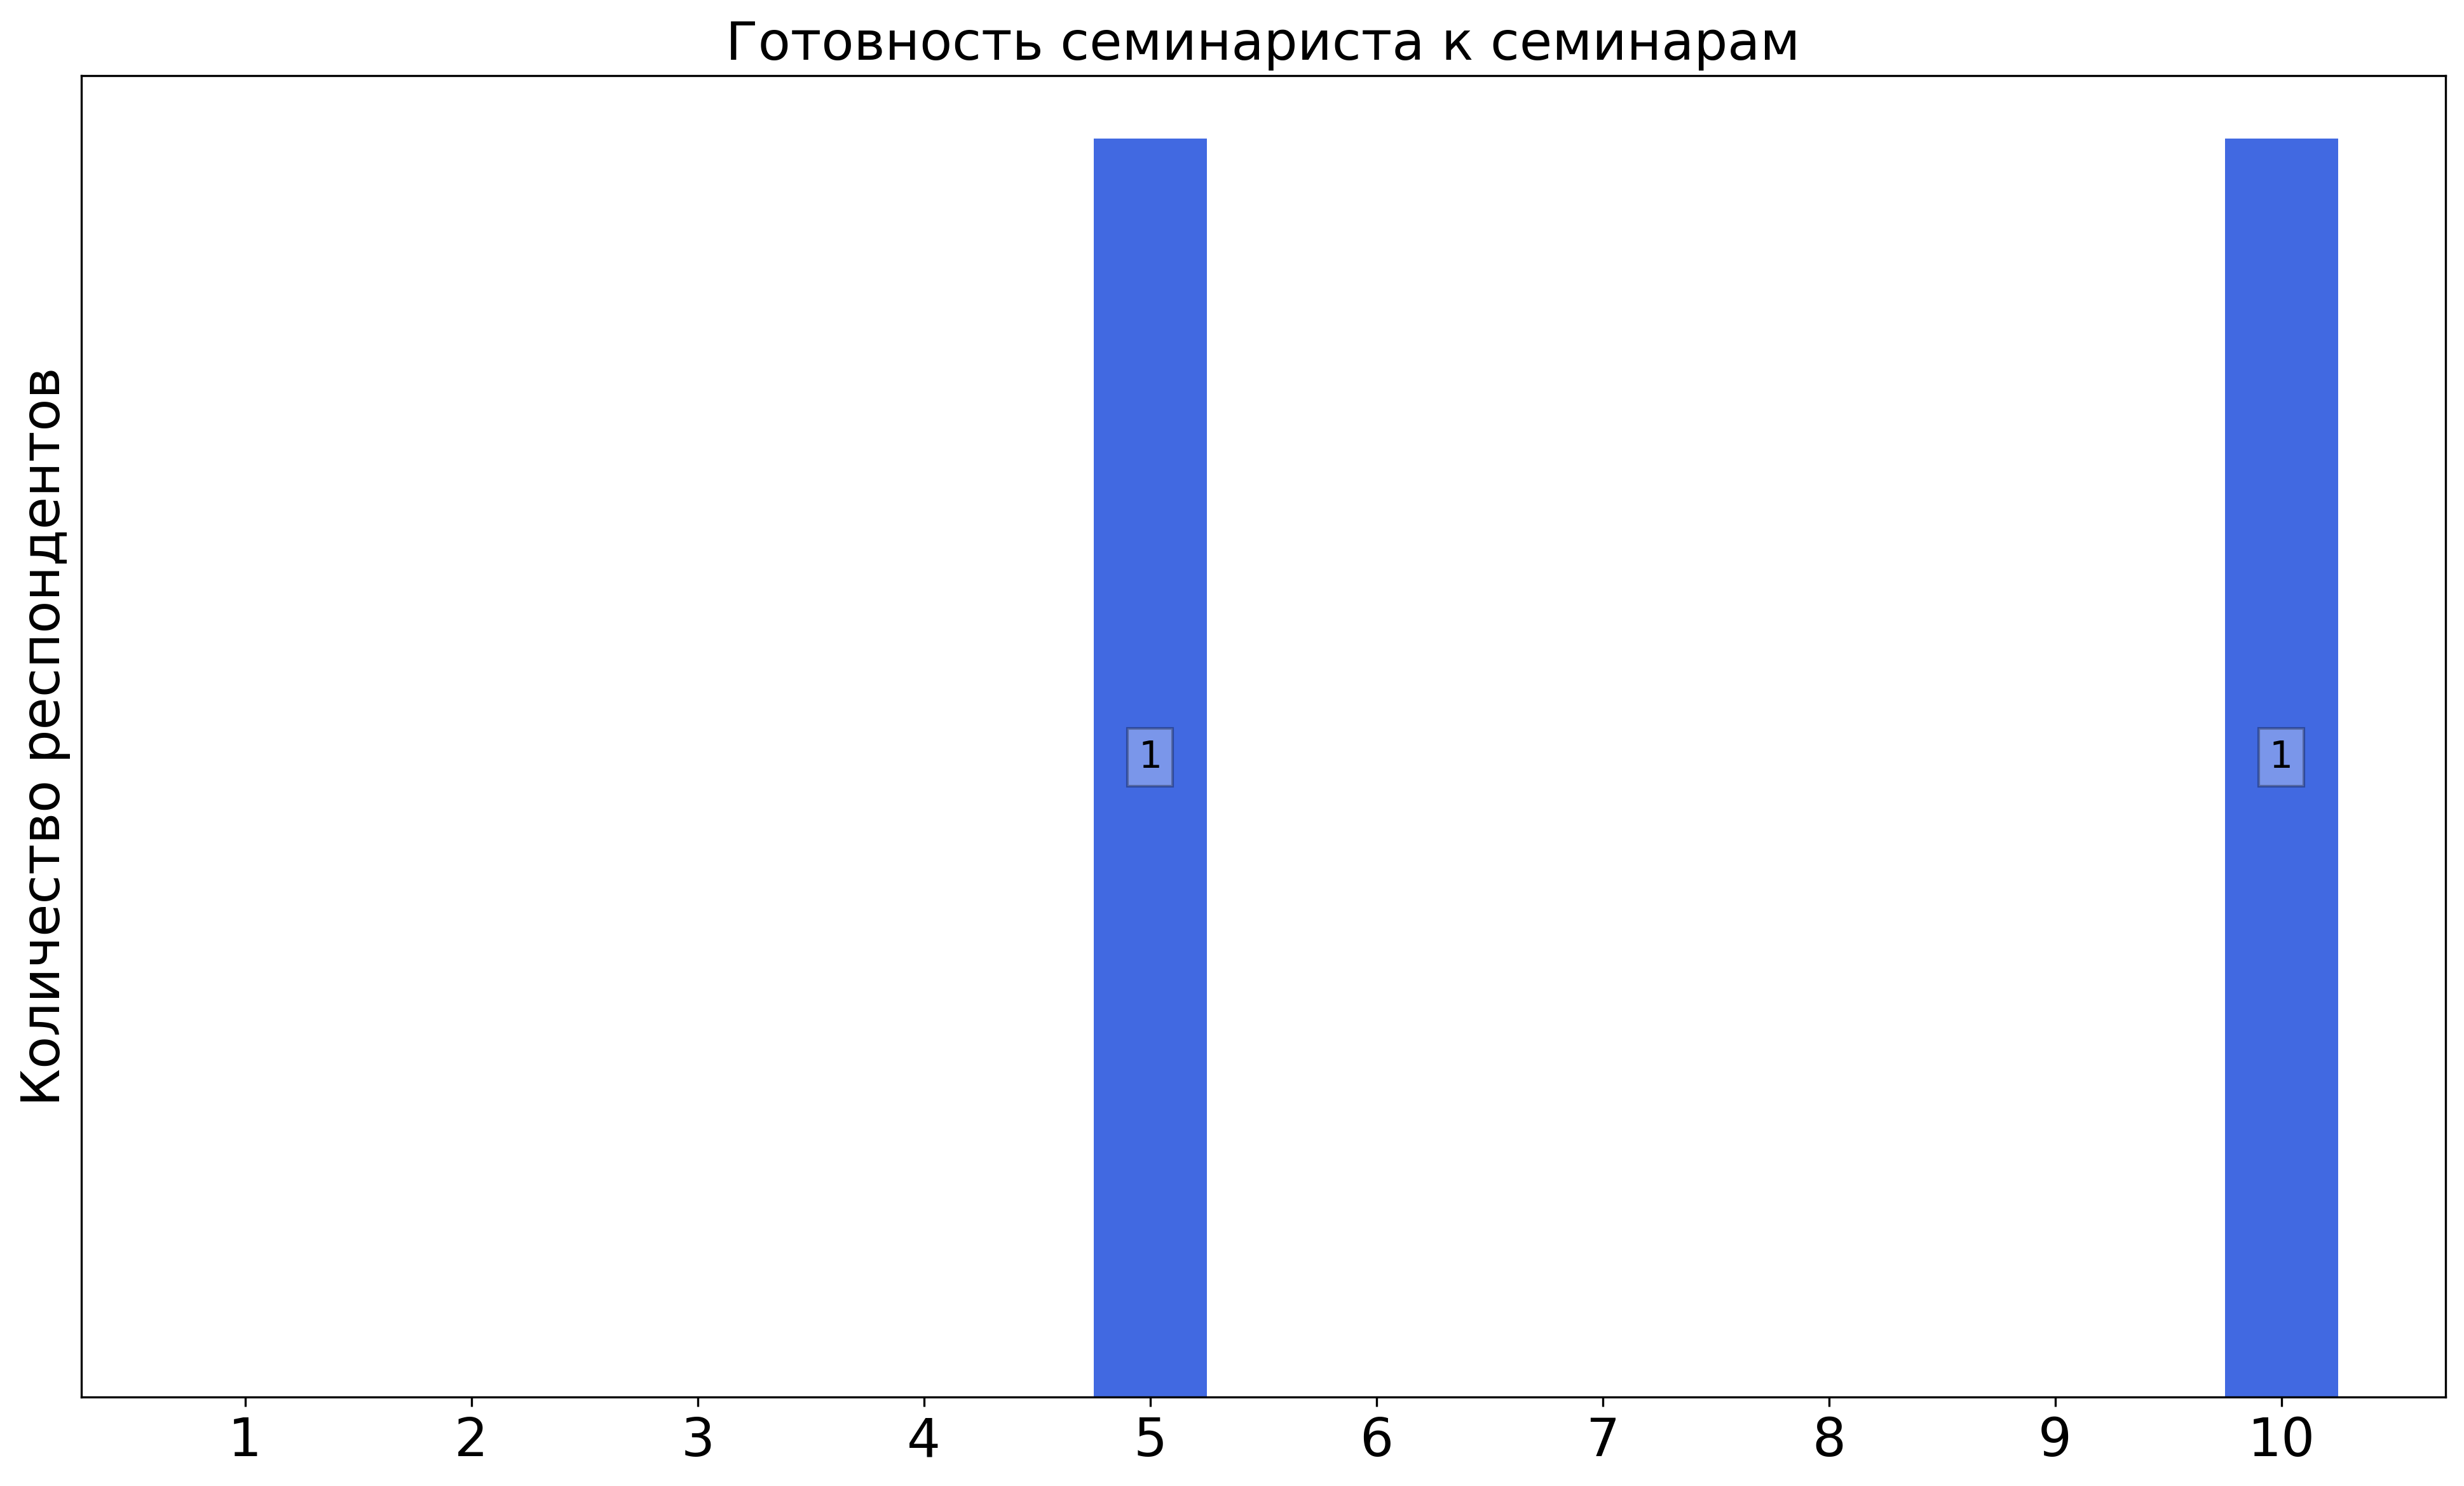
\includegraphics[width=\textwidth]{images/2 course/Компьютерные технологии/seminarists-marks-Гутник С.А.-1.png}
			\end{subfigure}
			\begin{subfigure}[b]{0.45\textwidth}
				\centering
				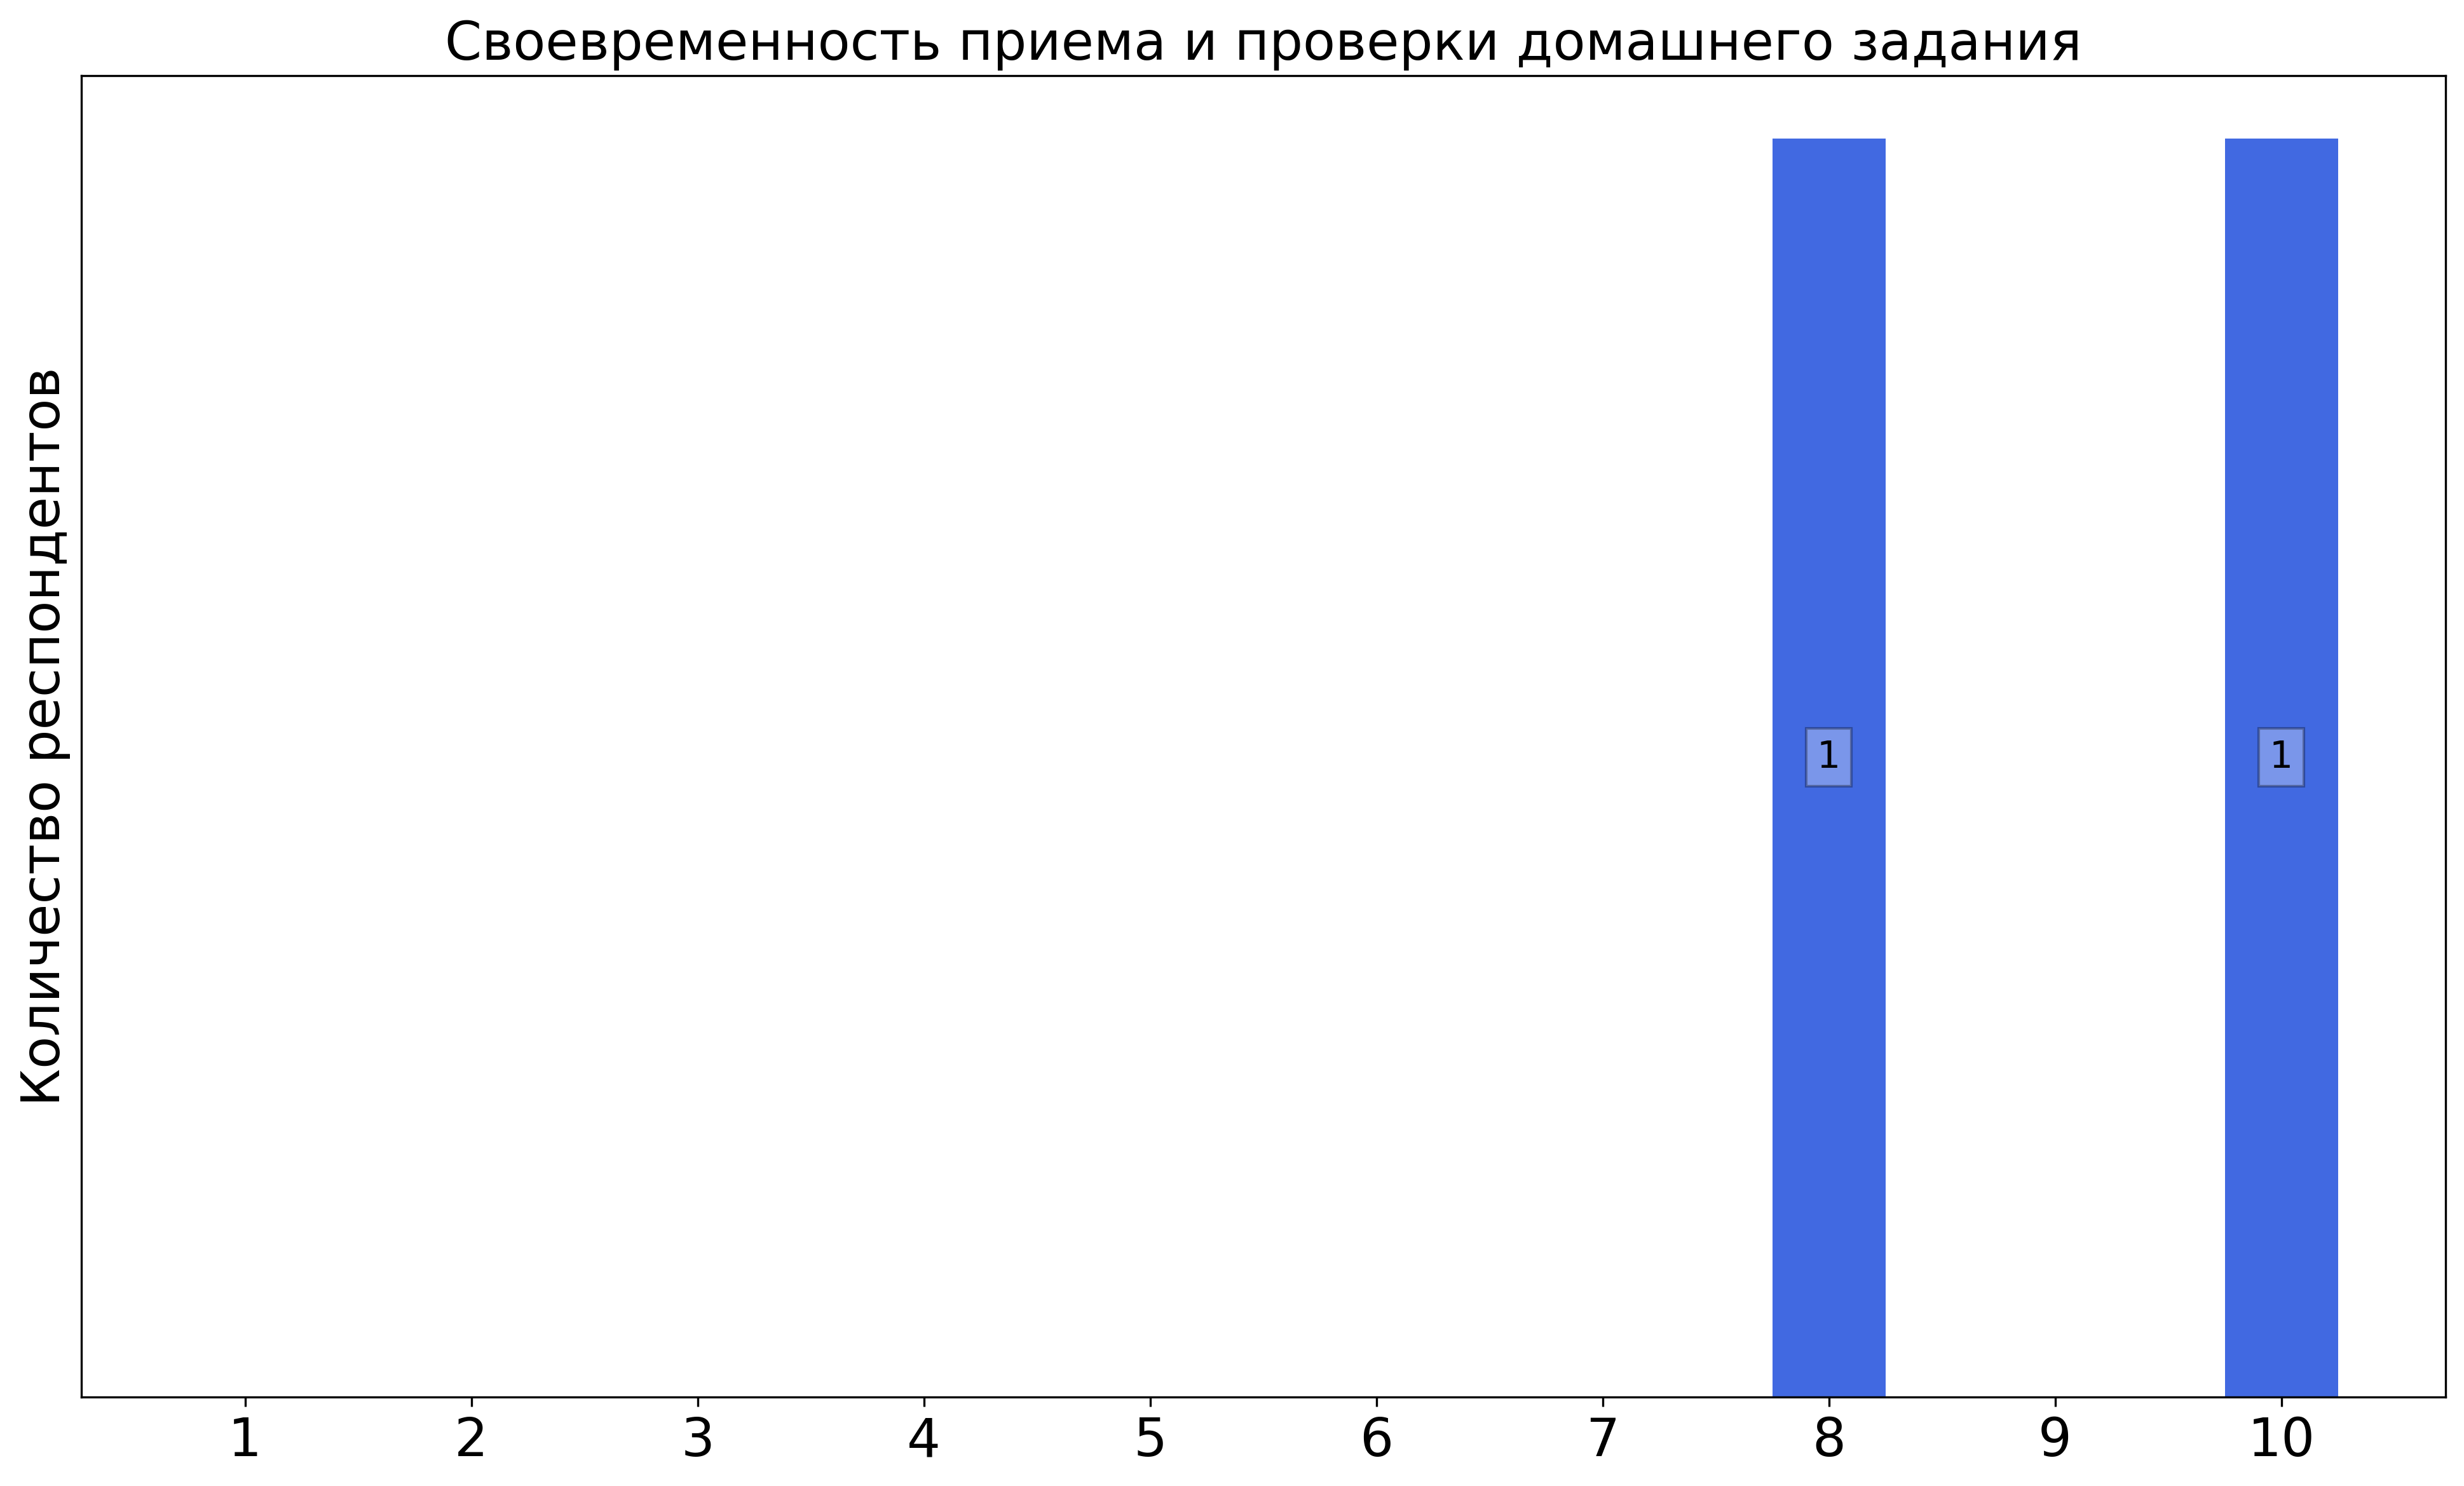
\includegraphics[width=\textwidth]{images/2 course/Компьютерные технологии/seminarists-marks-Гутник С.А.-2.png}
			\end{subfigure}
			\begin{subfigure}[b]{0.45\textwidth}
				\centering
				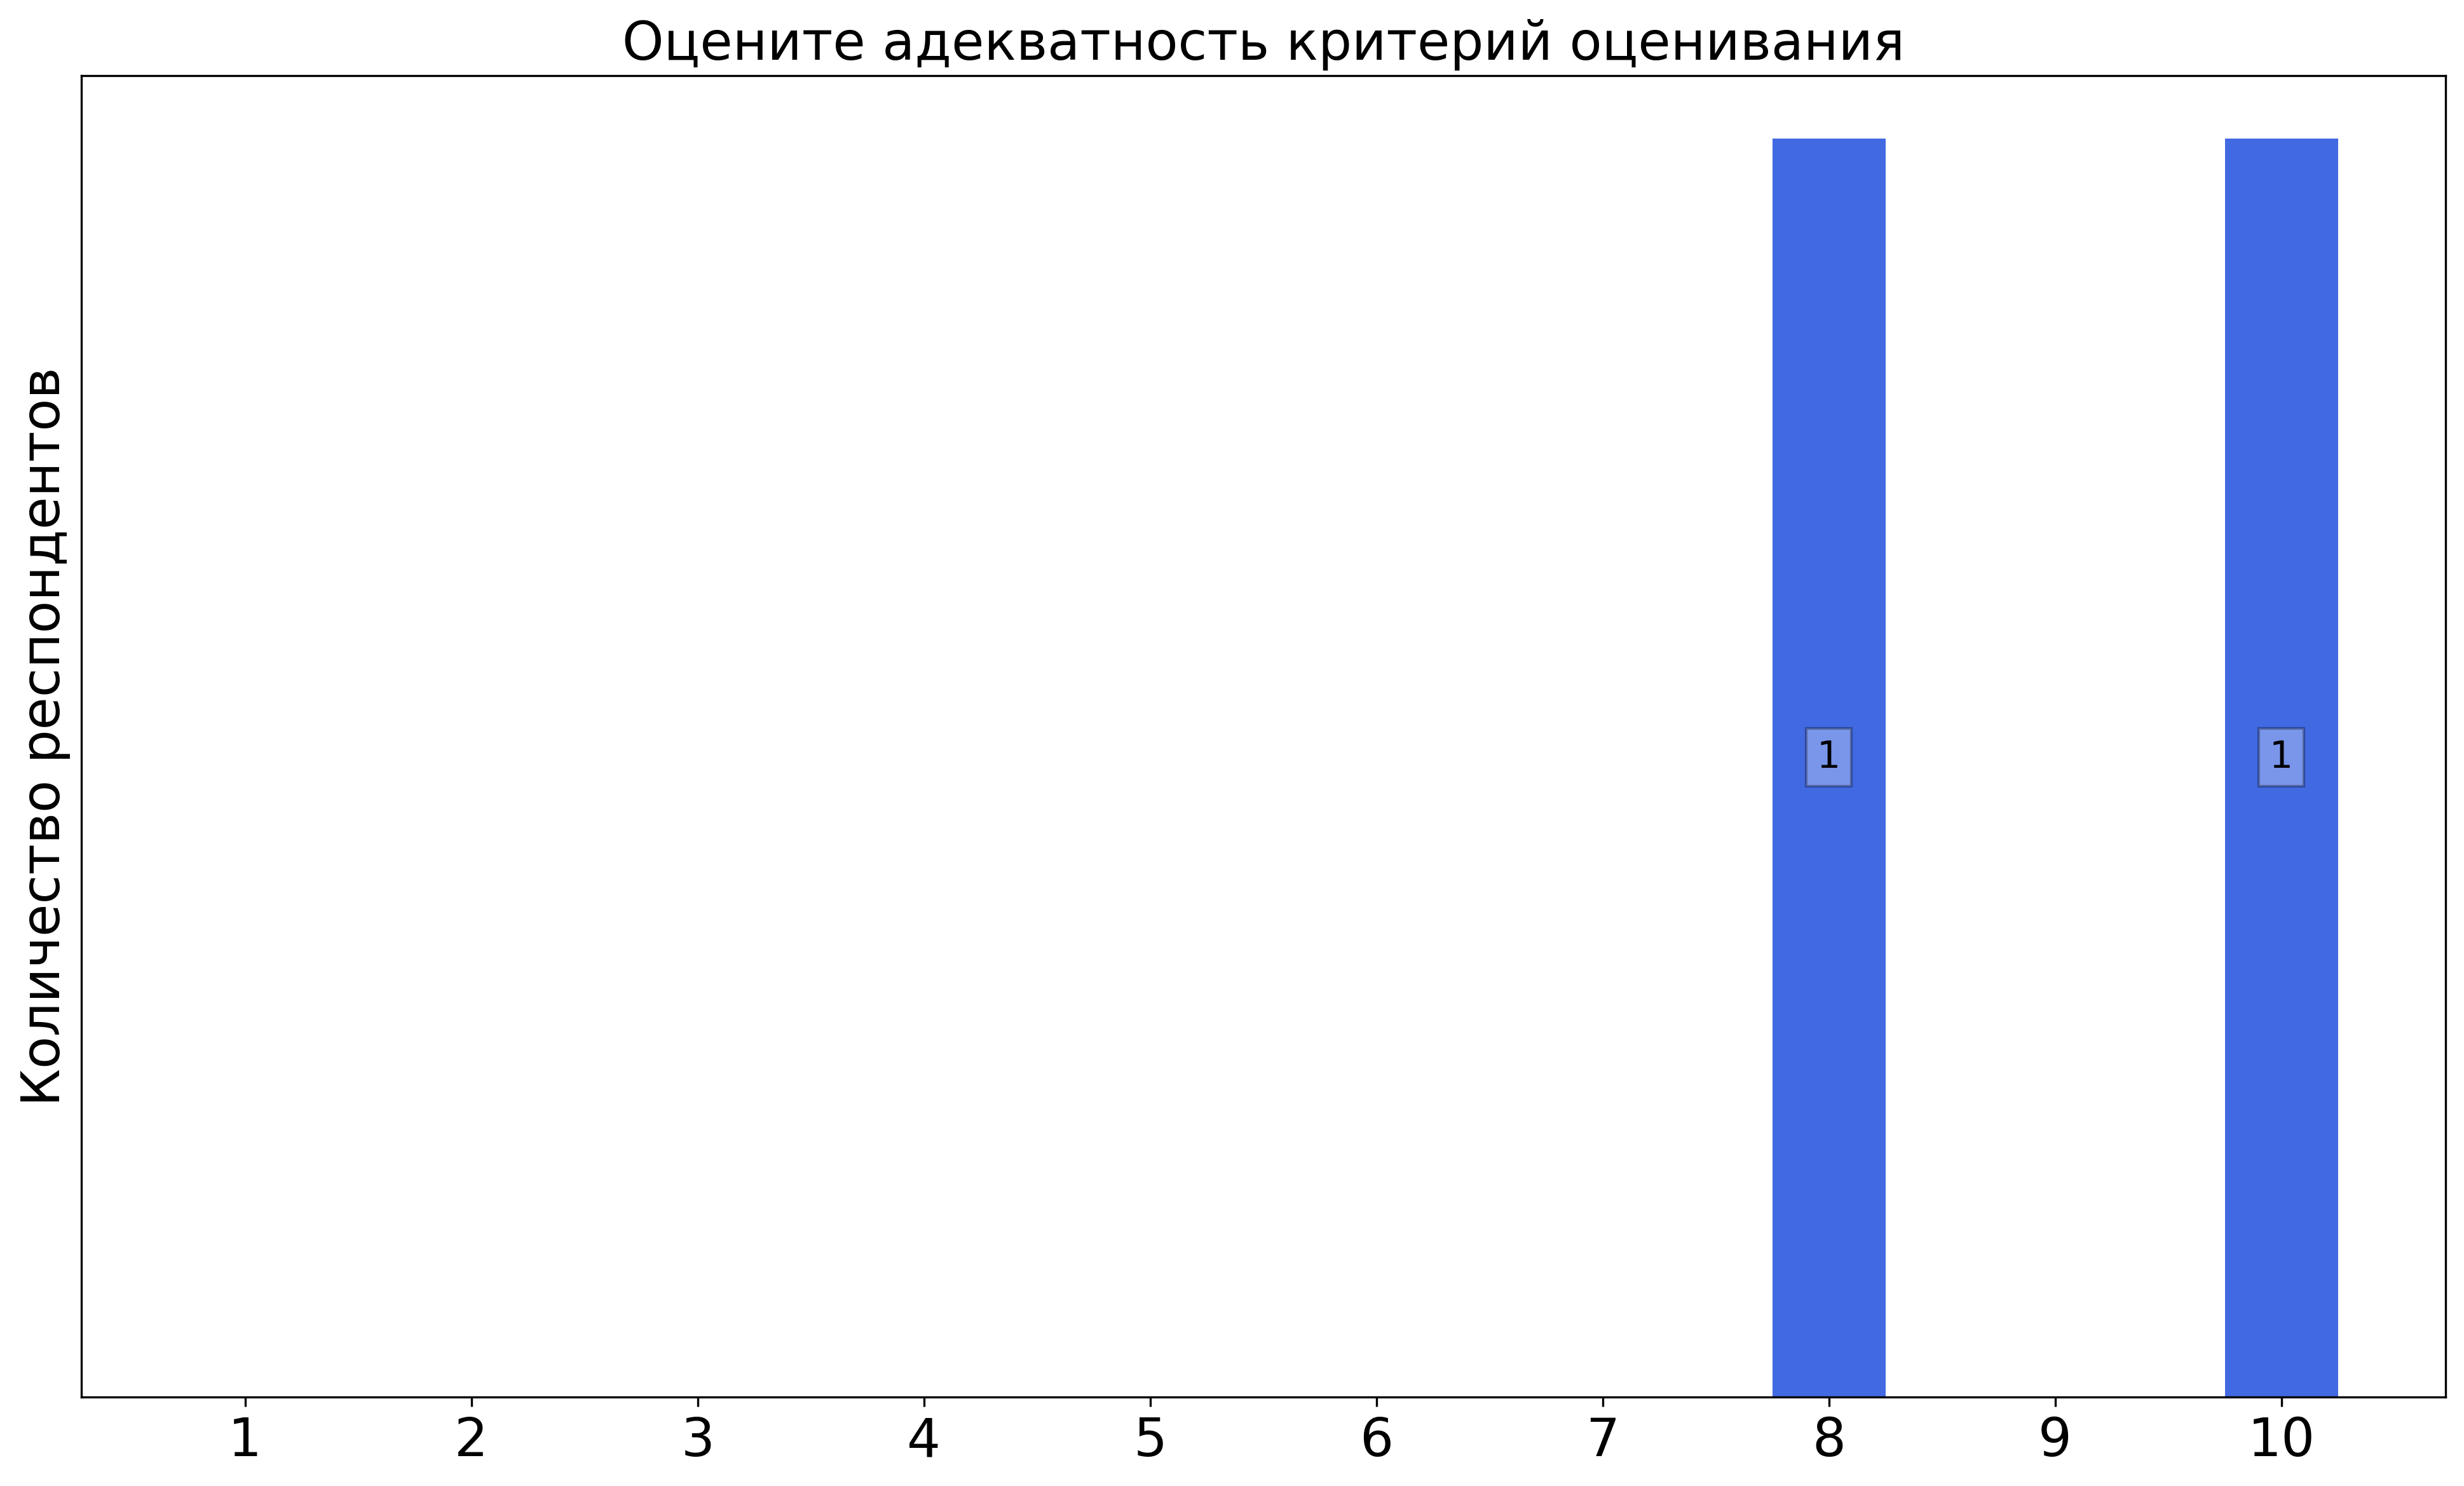
\includegraphics[width=\textwidth]{images/2 course/Компьютерные технологии/seminarists-marks-Гутник С.А.-3.png}
			\end{subfigure}	
			\caption{Оценки респондентов о качестве преподавания семинаров}
		\end{figure}

		\textbf{Комментарии студентов о семинаристе\protect\footnote{сохранены оригинальные орфография и пунктуация}}
            \begin{commentbox} 
                Очень странно рассказывает материал. Задания на семинаре - скопируйте код, вставьте 
            \end{commentbox}
            

    \subsubsection{Отзыв студентов о семинарах. Семинарист: Ефанов Н.Н.}
        \begin{figure}[H]
            \centering
            \begin{subfigure}[b]{0.45\textwidth}
                \centering
                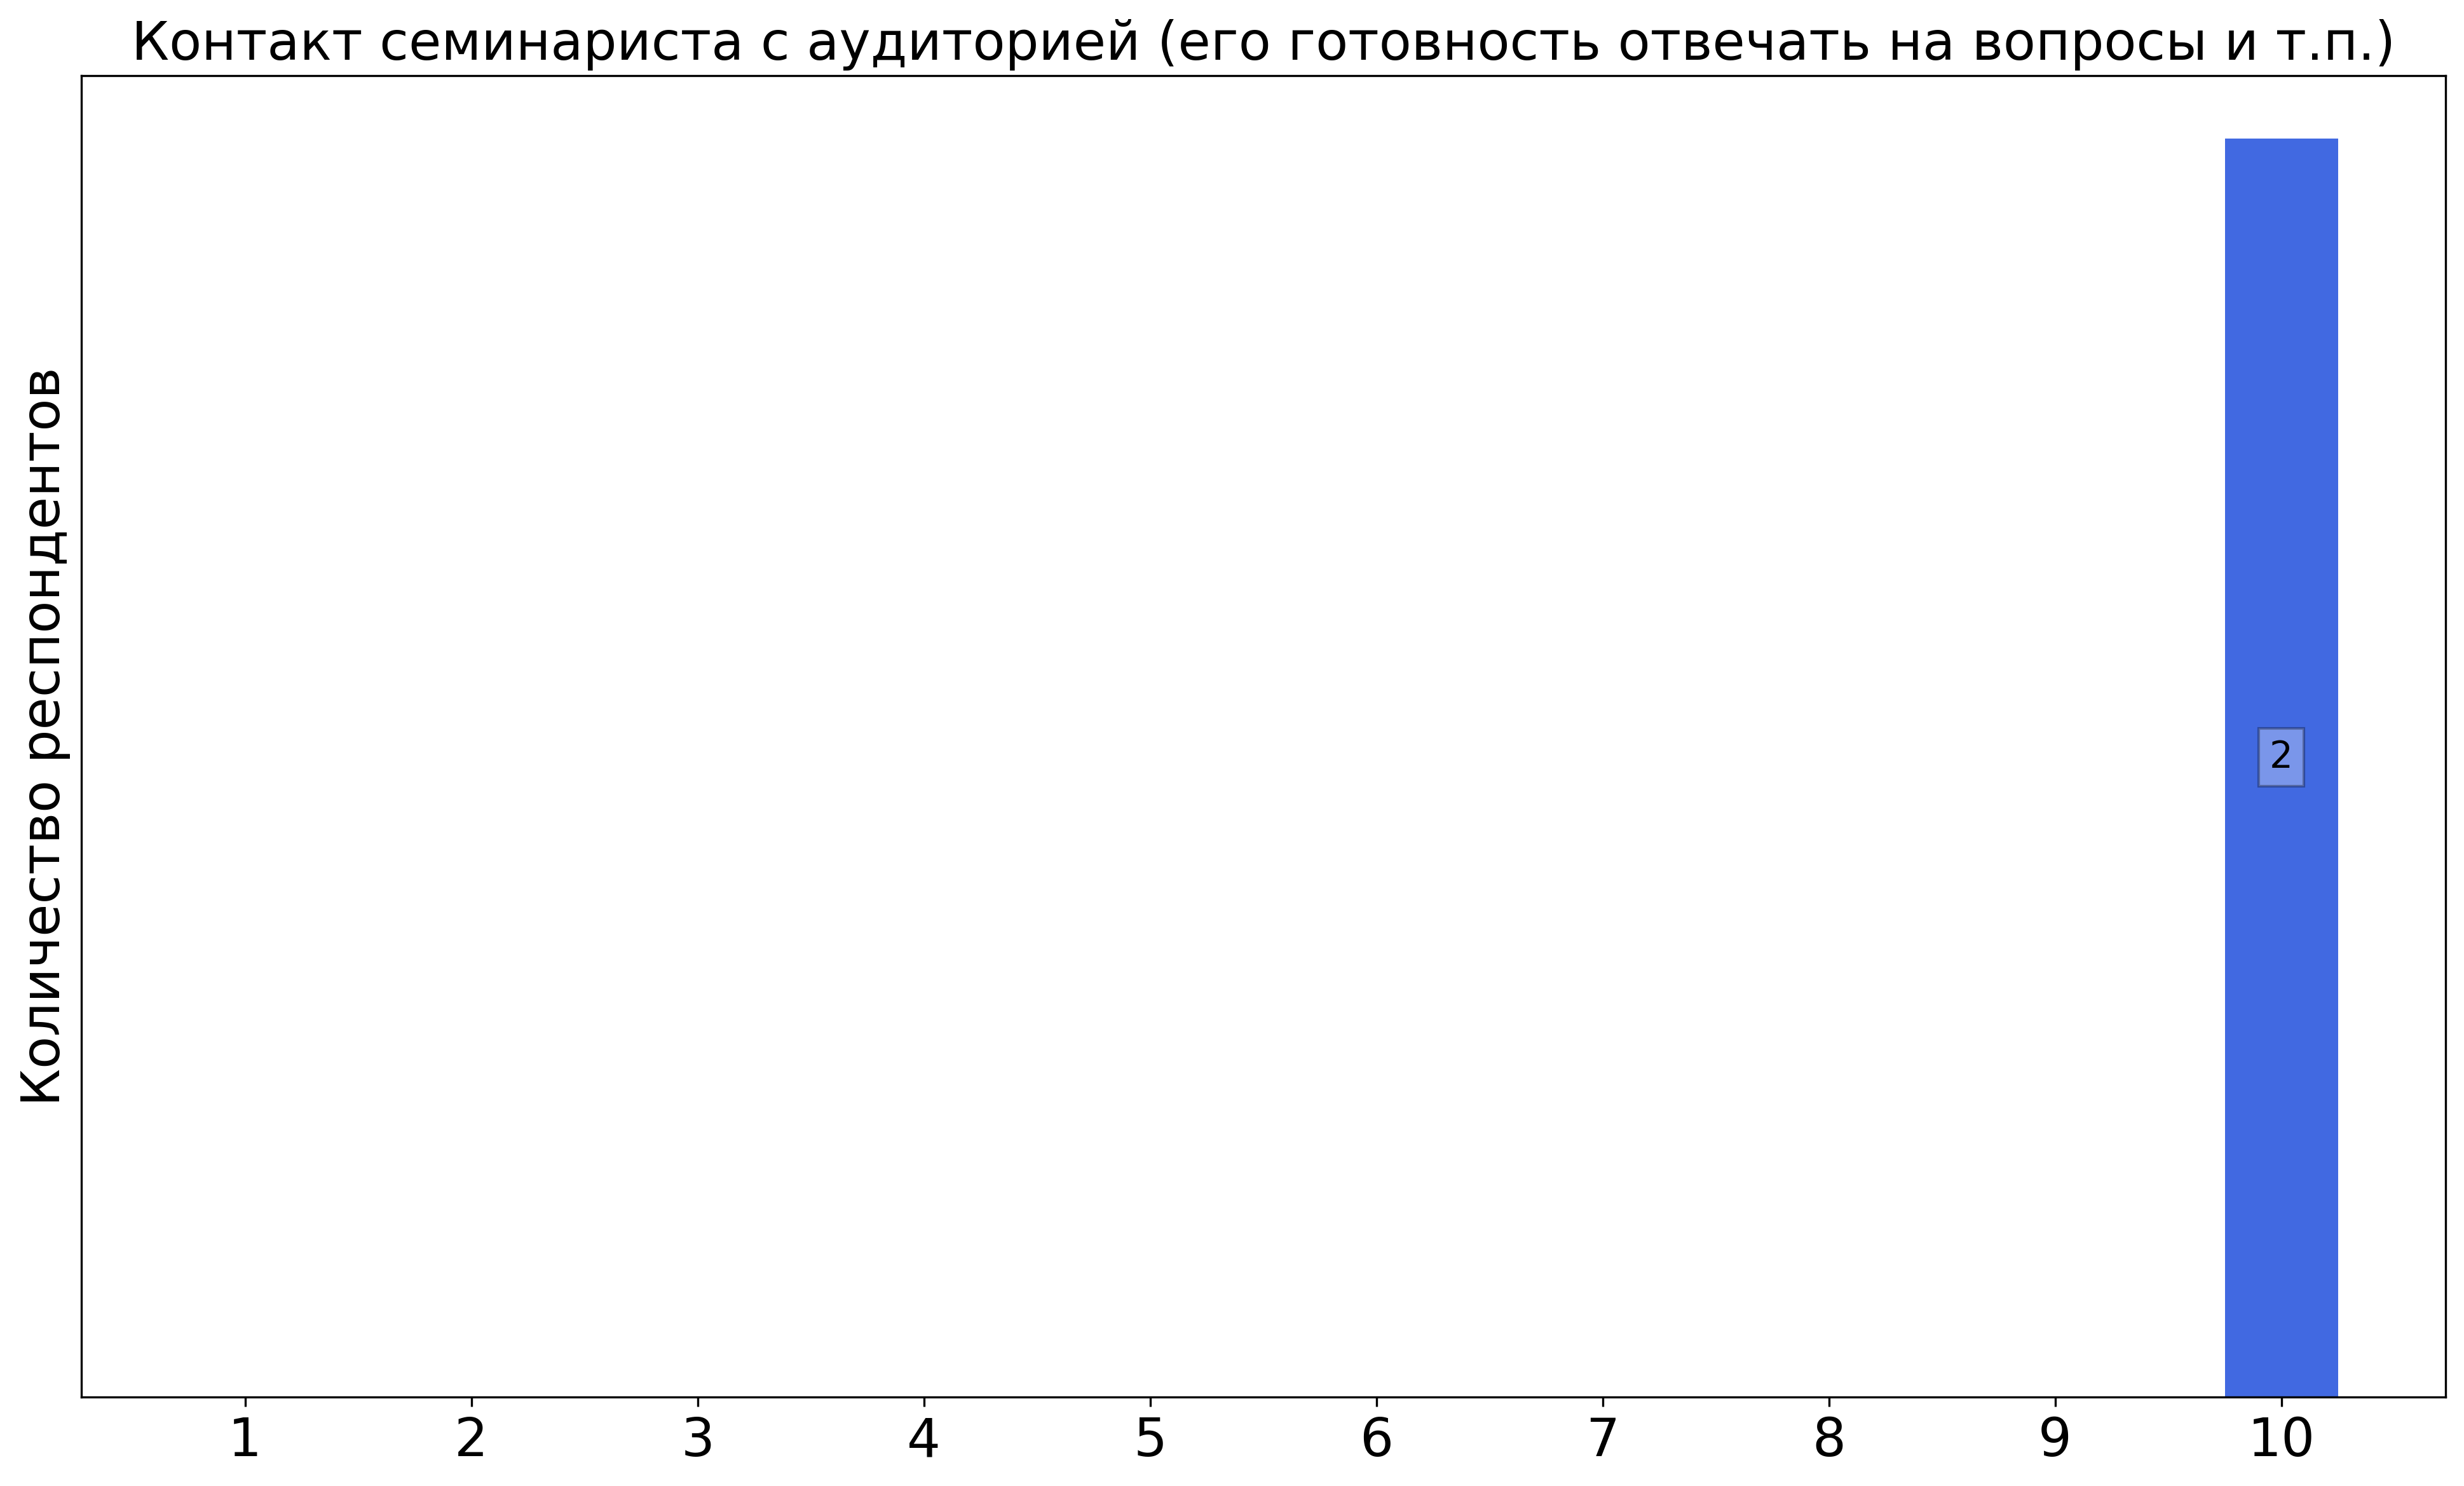
\includegraphics[width=\textwidth]{images/2 course/Компьютерные технологии/seminarists-marks-Ефанов Н.Н.-0.png}
            \end{subfigure}
            \begin{subfigure}[b]{0.45\textwidth}
                \centering
                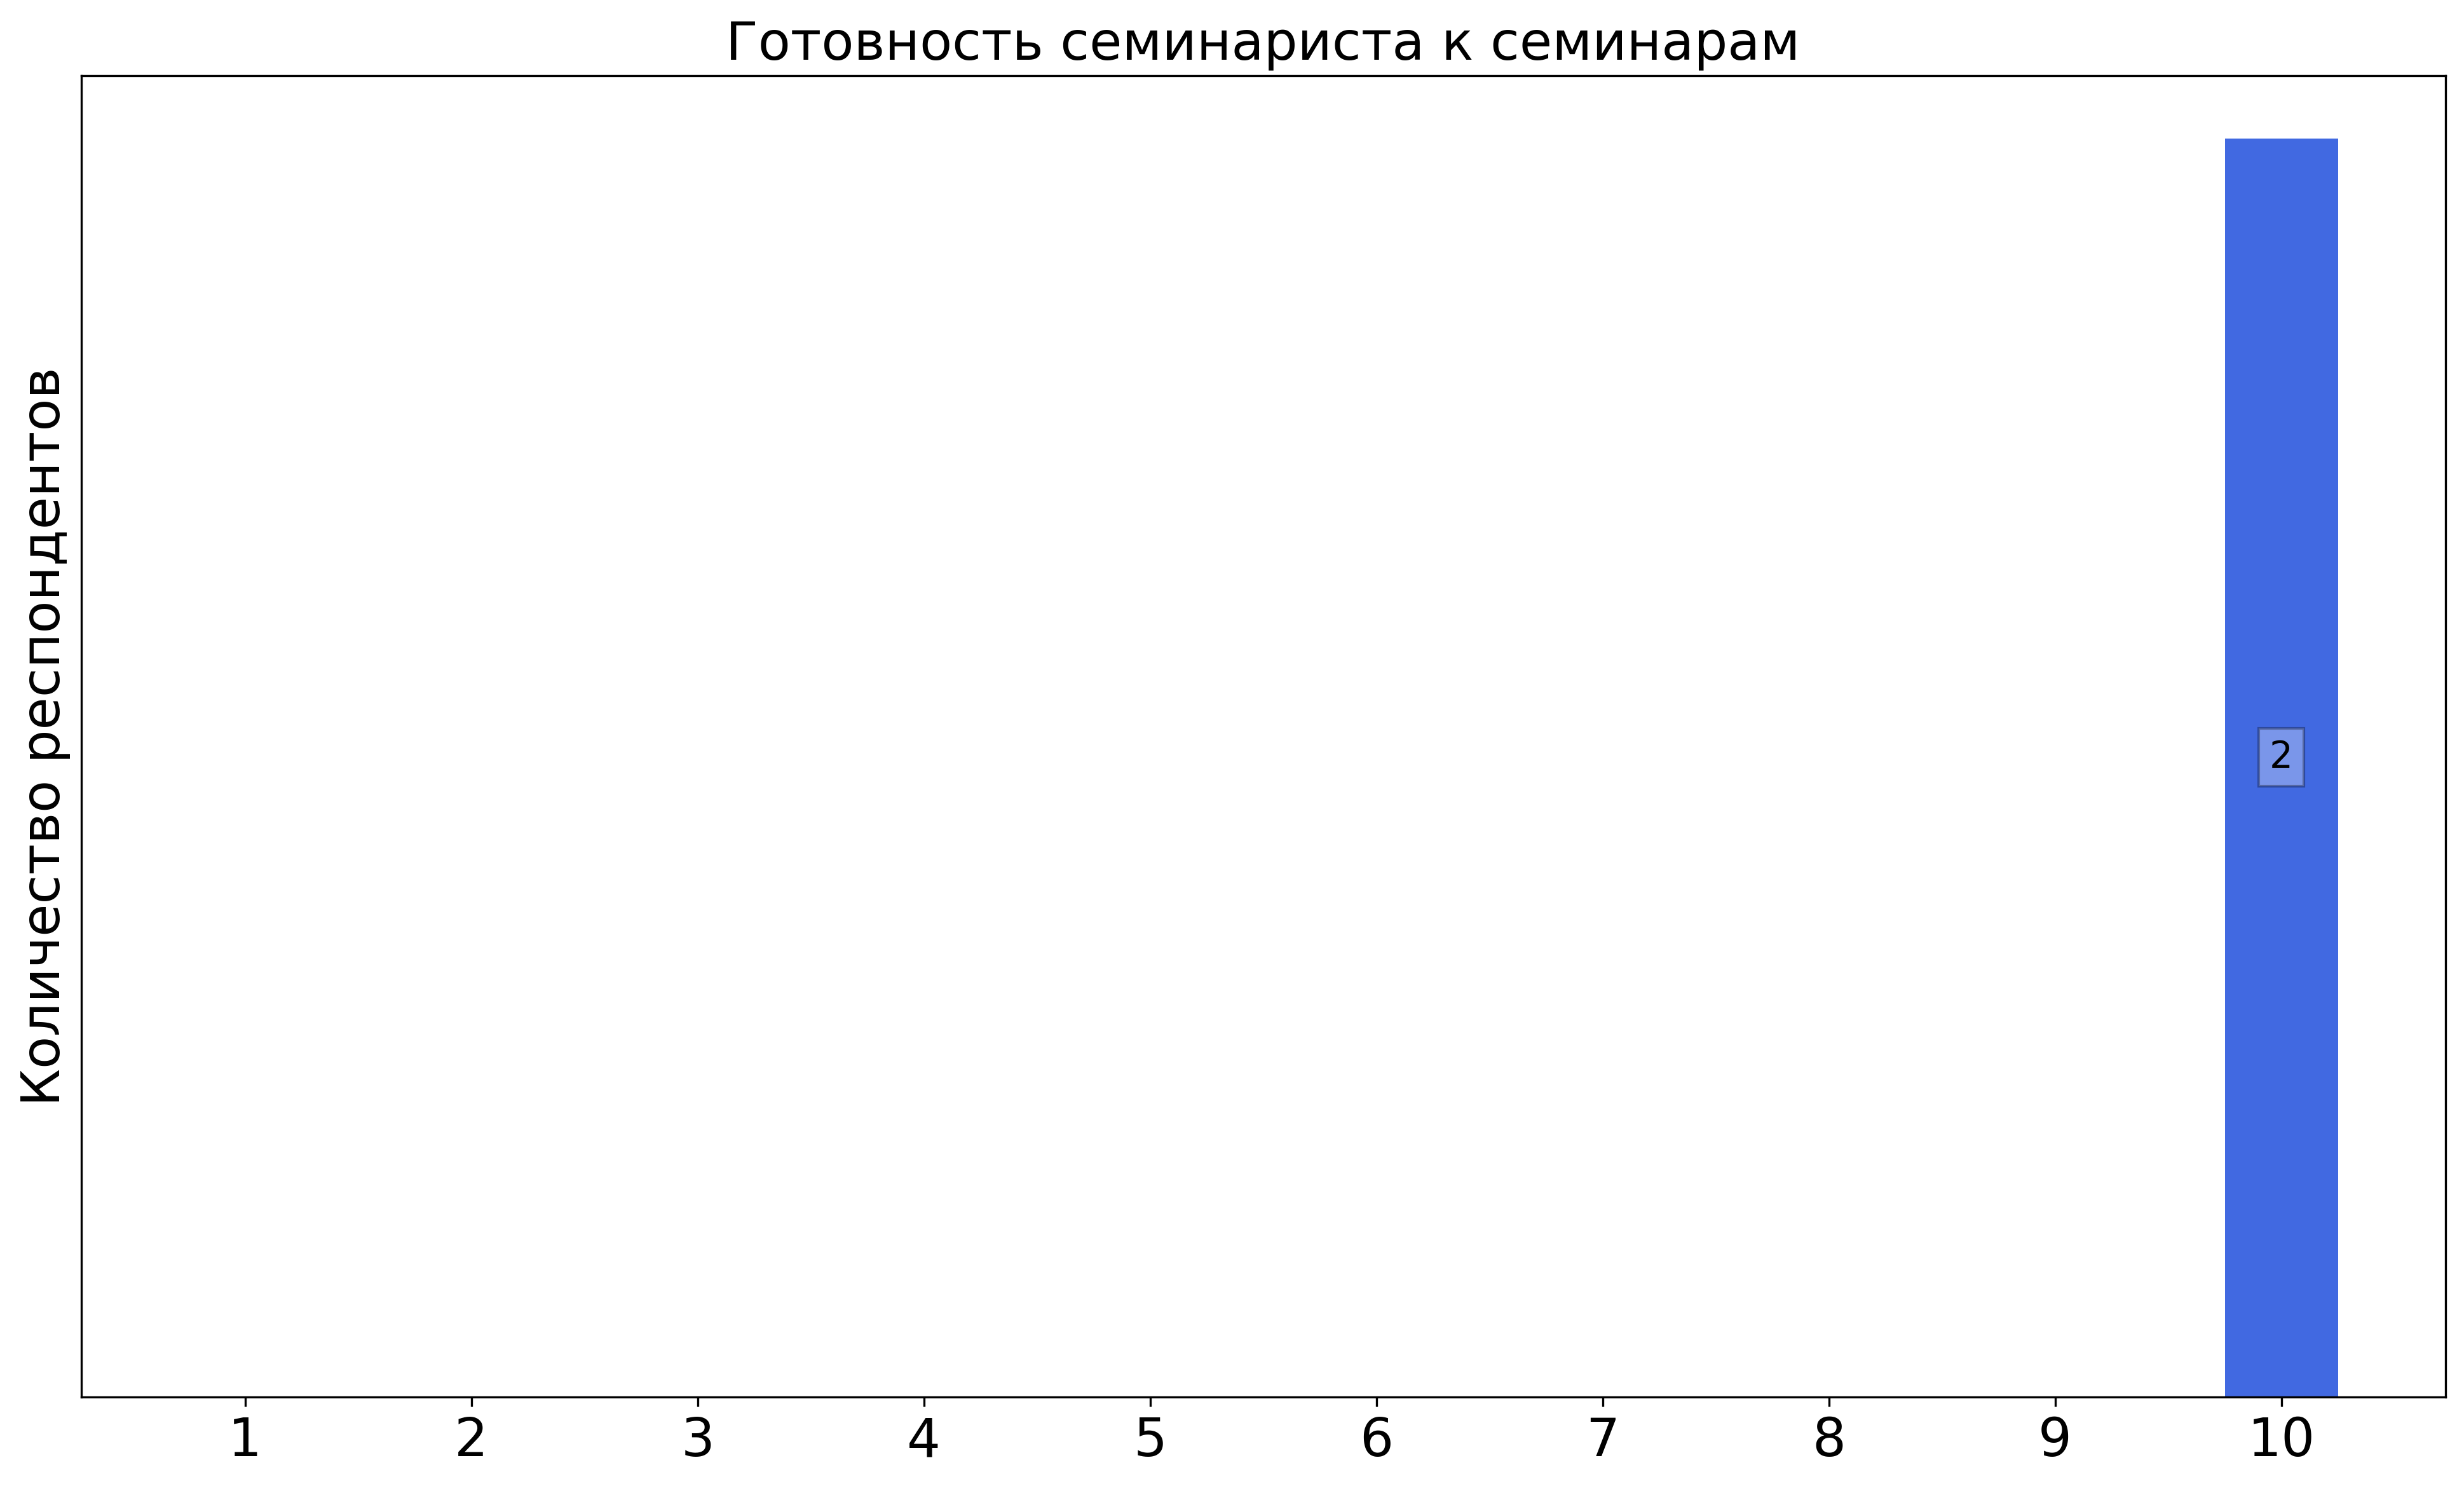
\includegraphics[width=\textwidth]{images/2 course/Компьютерные технологии/seminarists-marks-Ефанов Н.Н.-1.png}
            \end{subfigure}
            \begin{subfigure}[b]{0.45\textwidth}
                \centering
                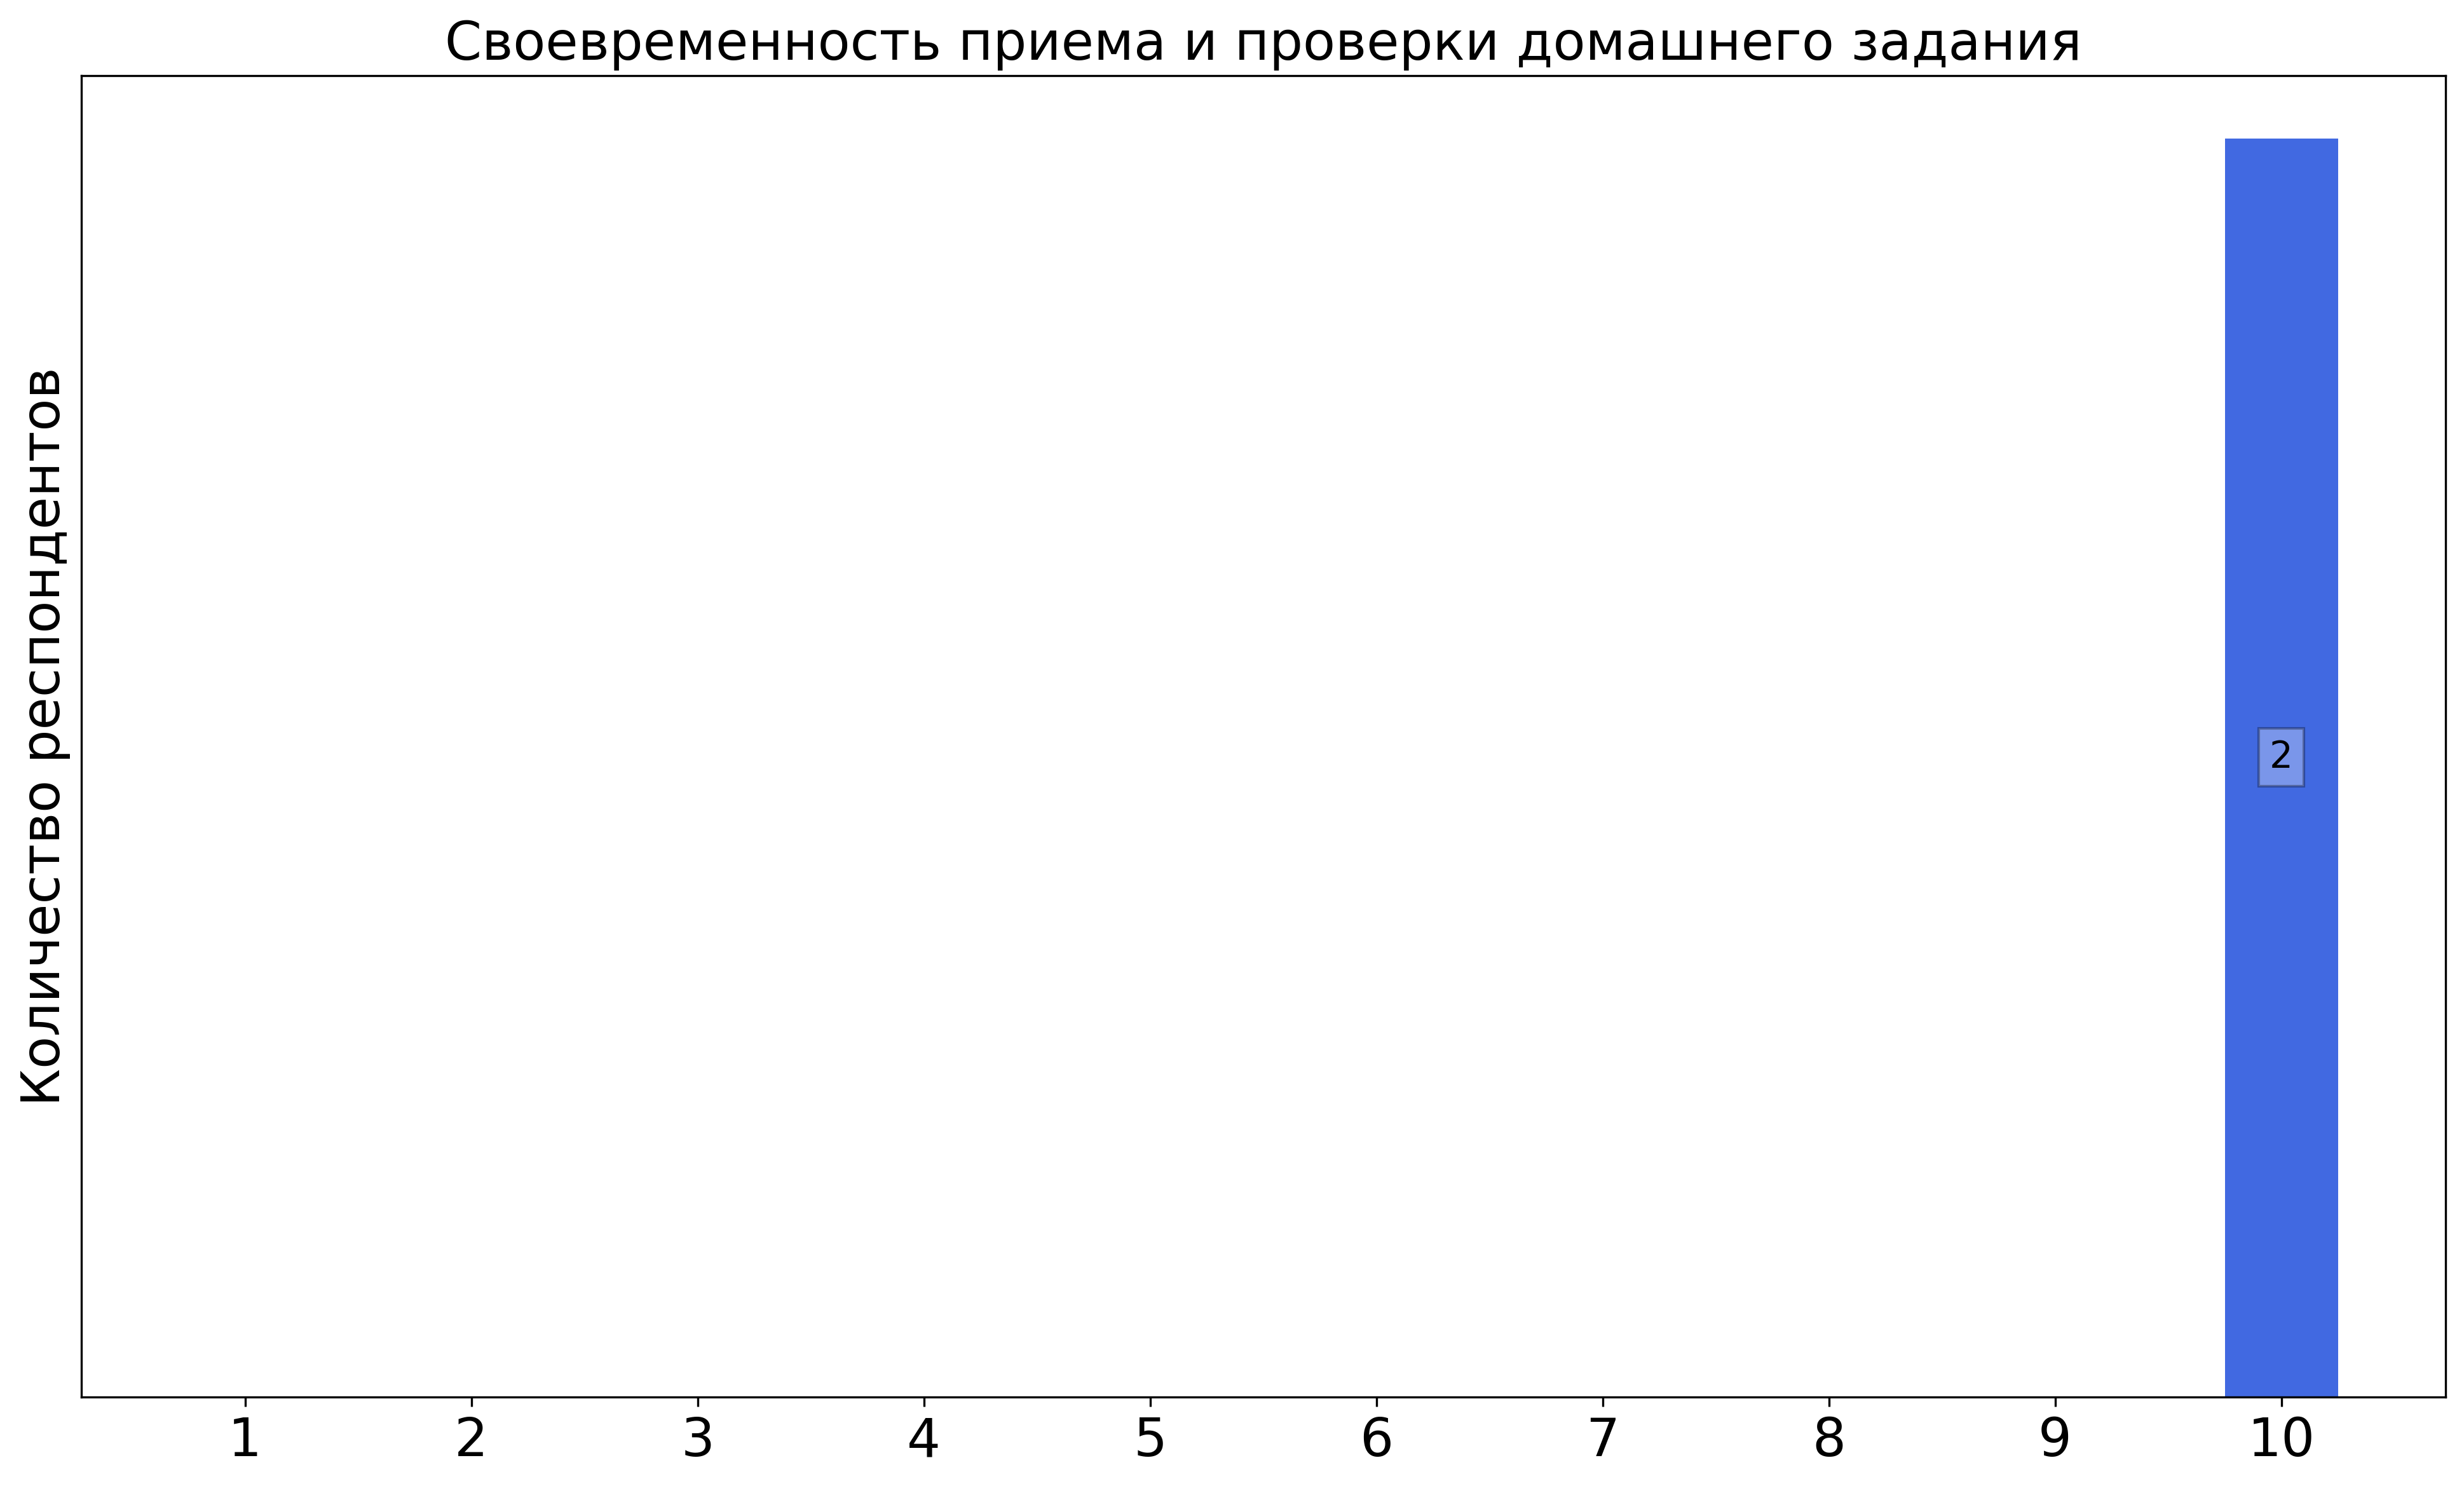
\includegraphics[width=\textwidth]{images/2 course/Компьютерные технологии/seminarists-marks-Ефанов Н.Н.-2.png}
            \end{subfigure}
            \begin{subfigure}[b]{0.45\textwidth}
                \centering
                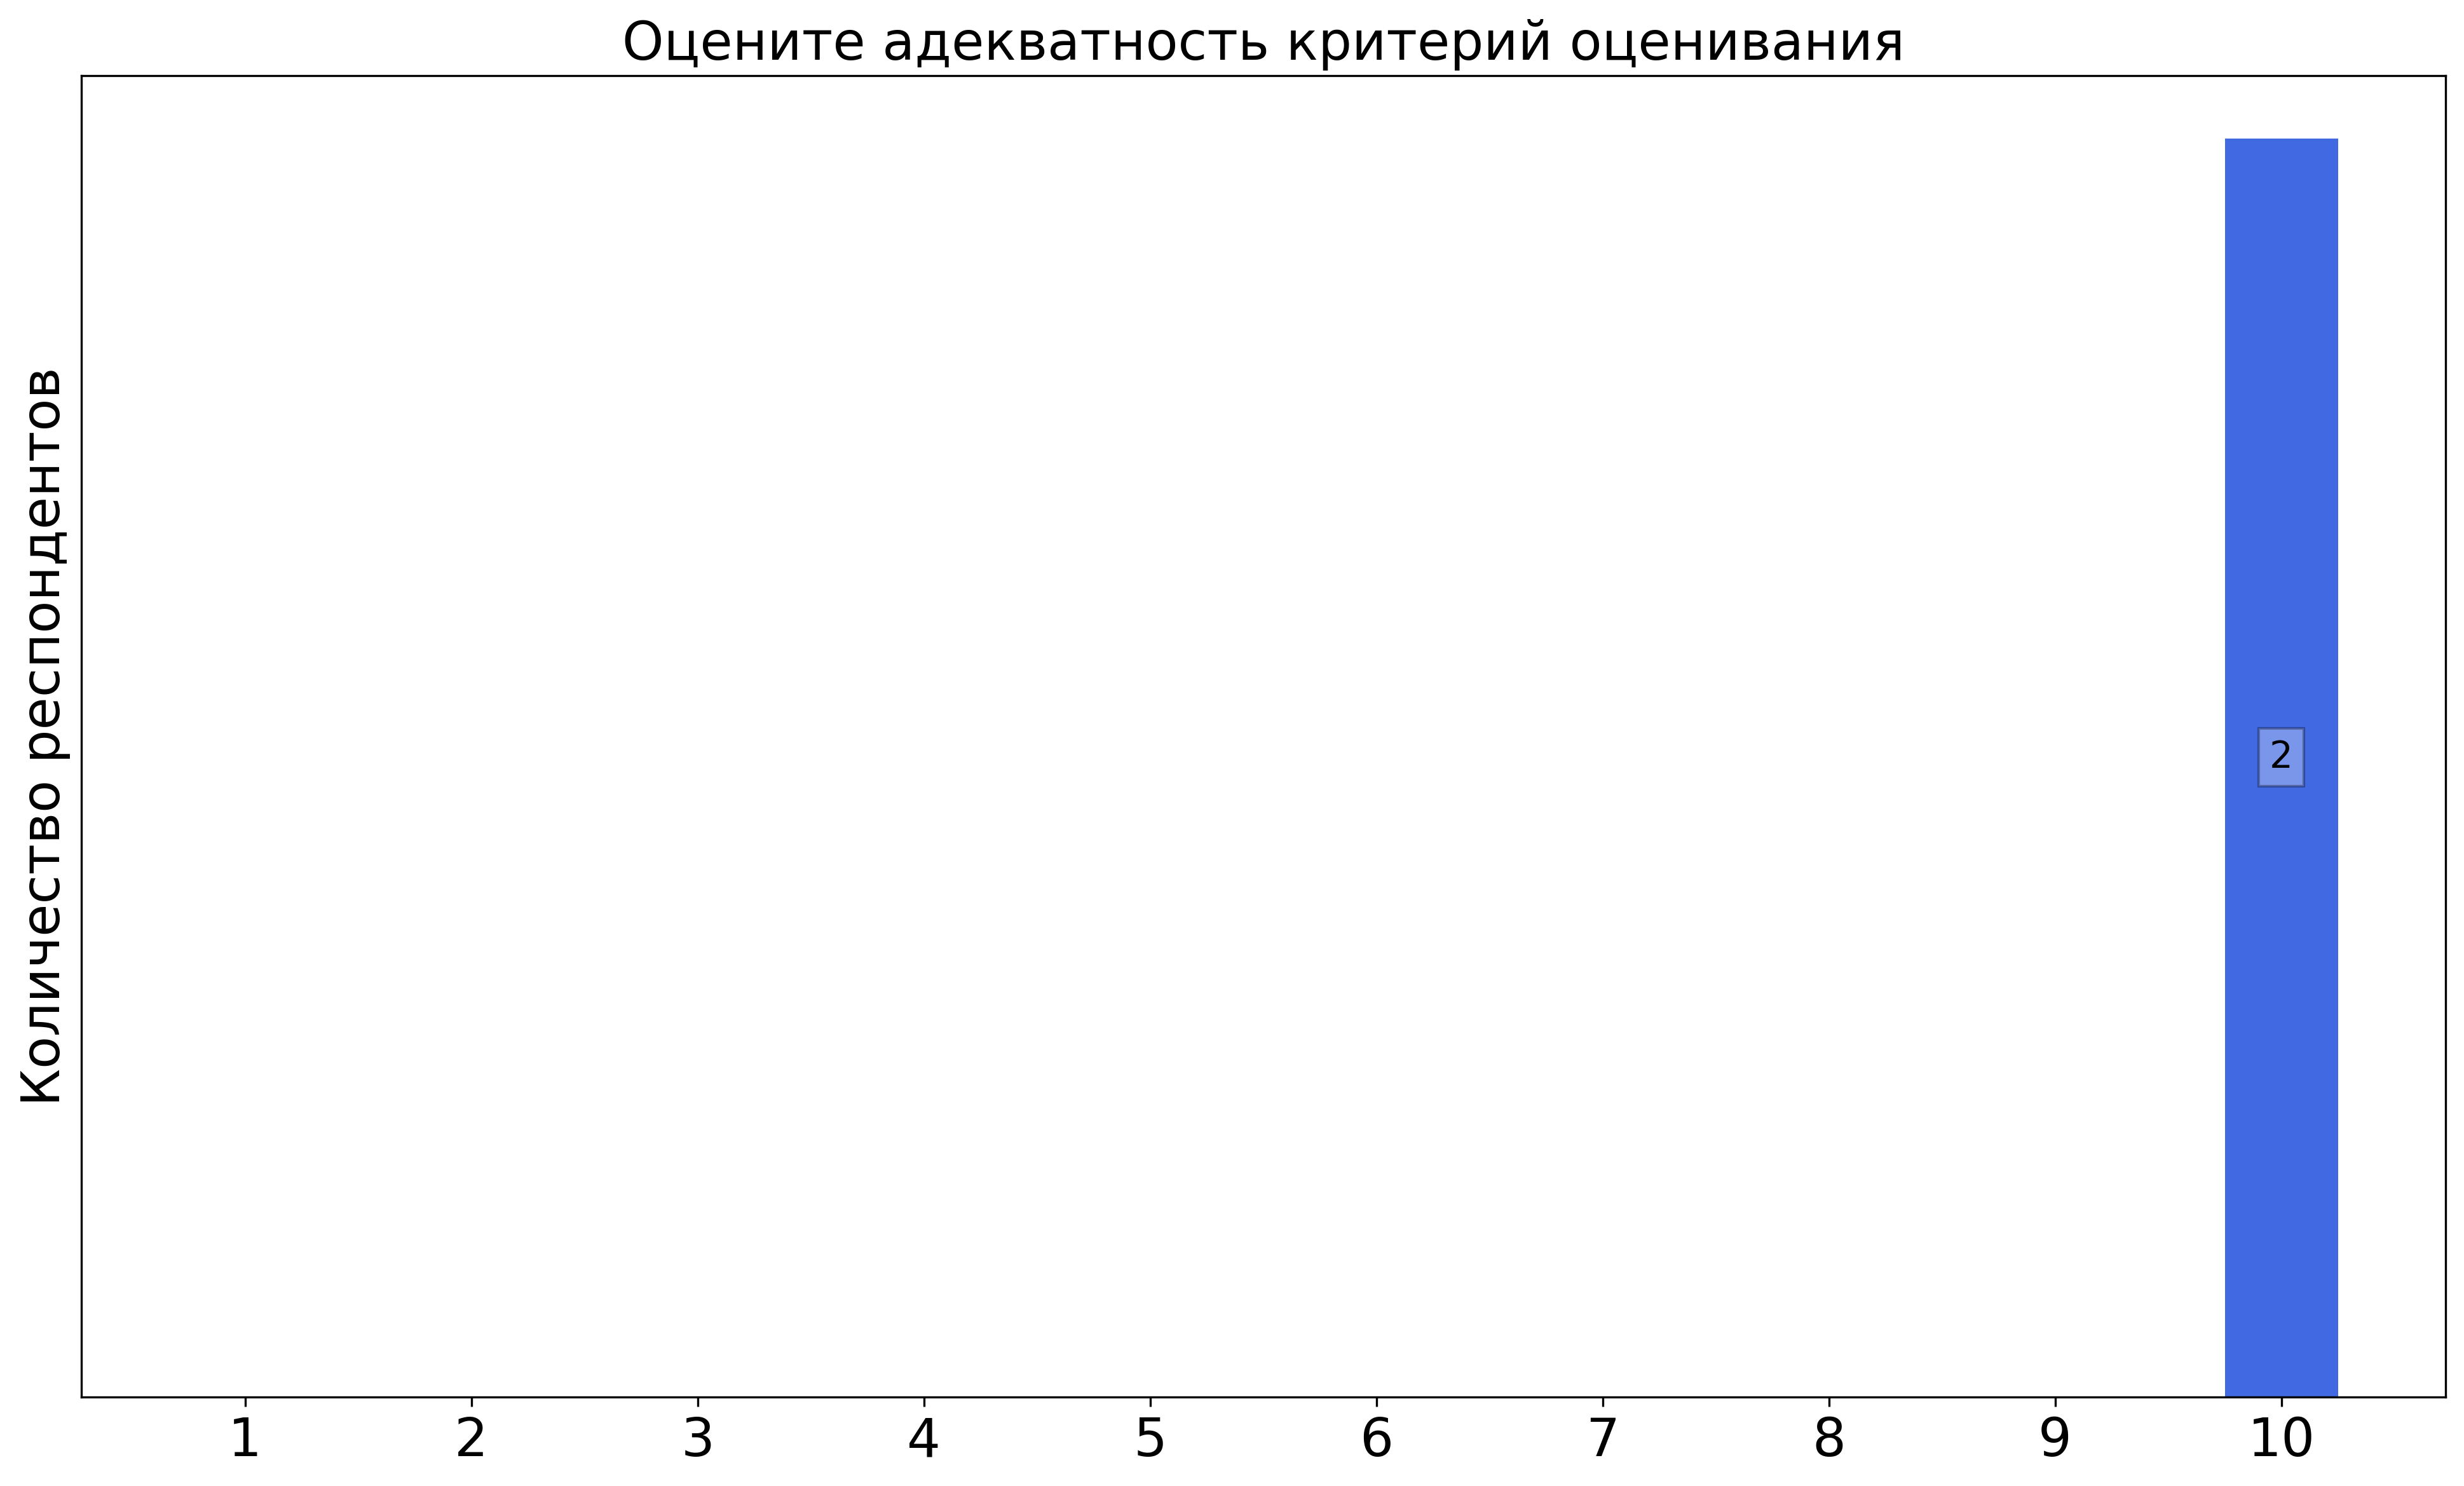
\includegraphics[width=\textwidth]{images/2 course/Компьютерные технологии/seminarists-marks-Ефанов Н.Н.-3.png}
            \end{subfigure}	
            \caption{Оценки респондентов о качестве преподавания семинаров}
        \end{figure}


        
    \subsubsection{Отзыв студентов о семинарах. Семинарист: Красильников Н.И.}
        \begin{figure}[H]
            \centering
            \begin{subfigure}[b]{0.45\textwidth}
                \centering
                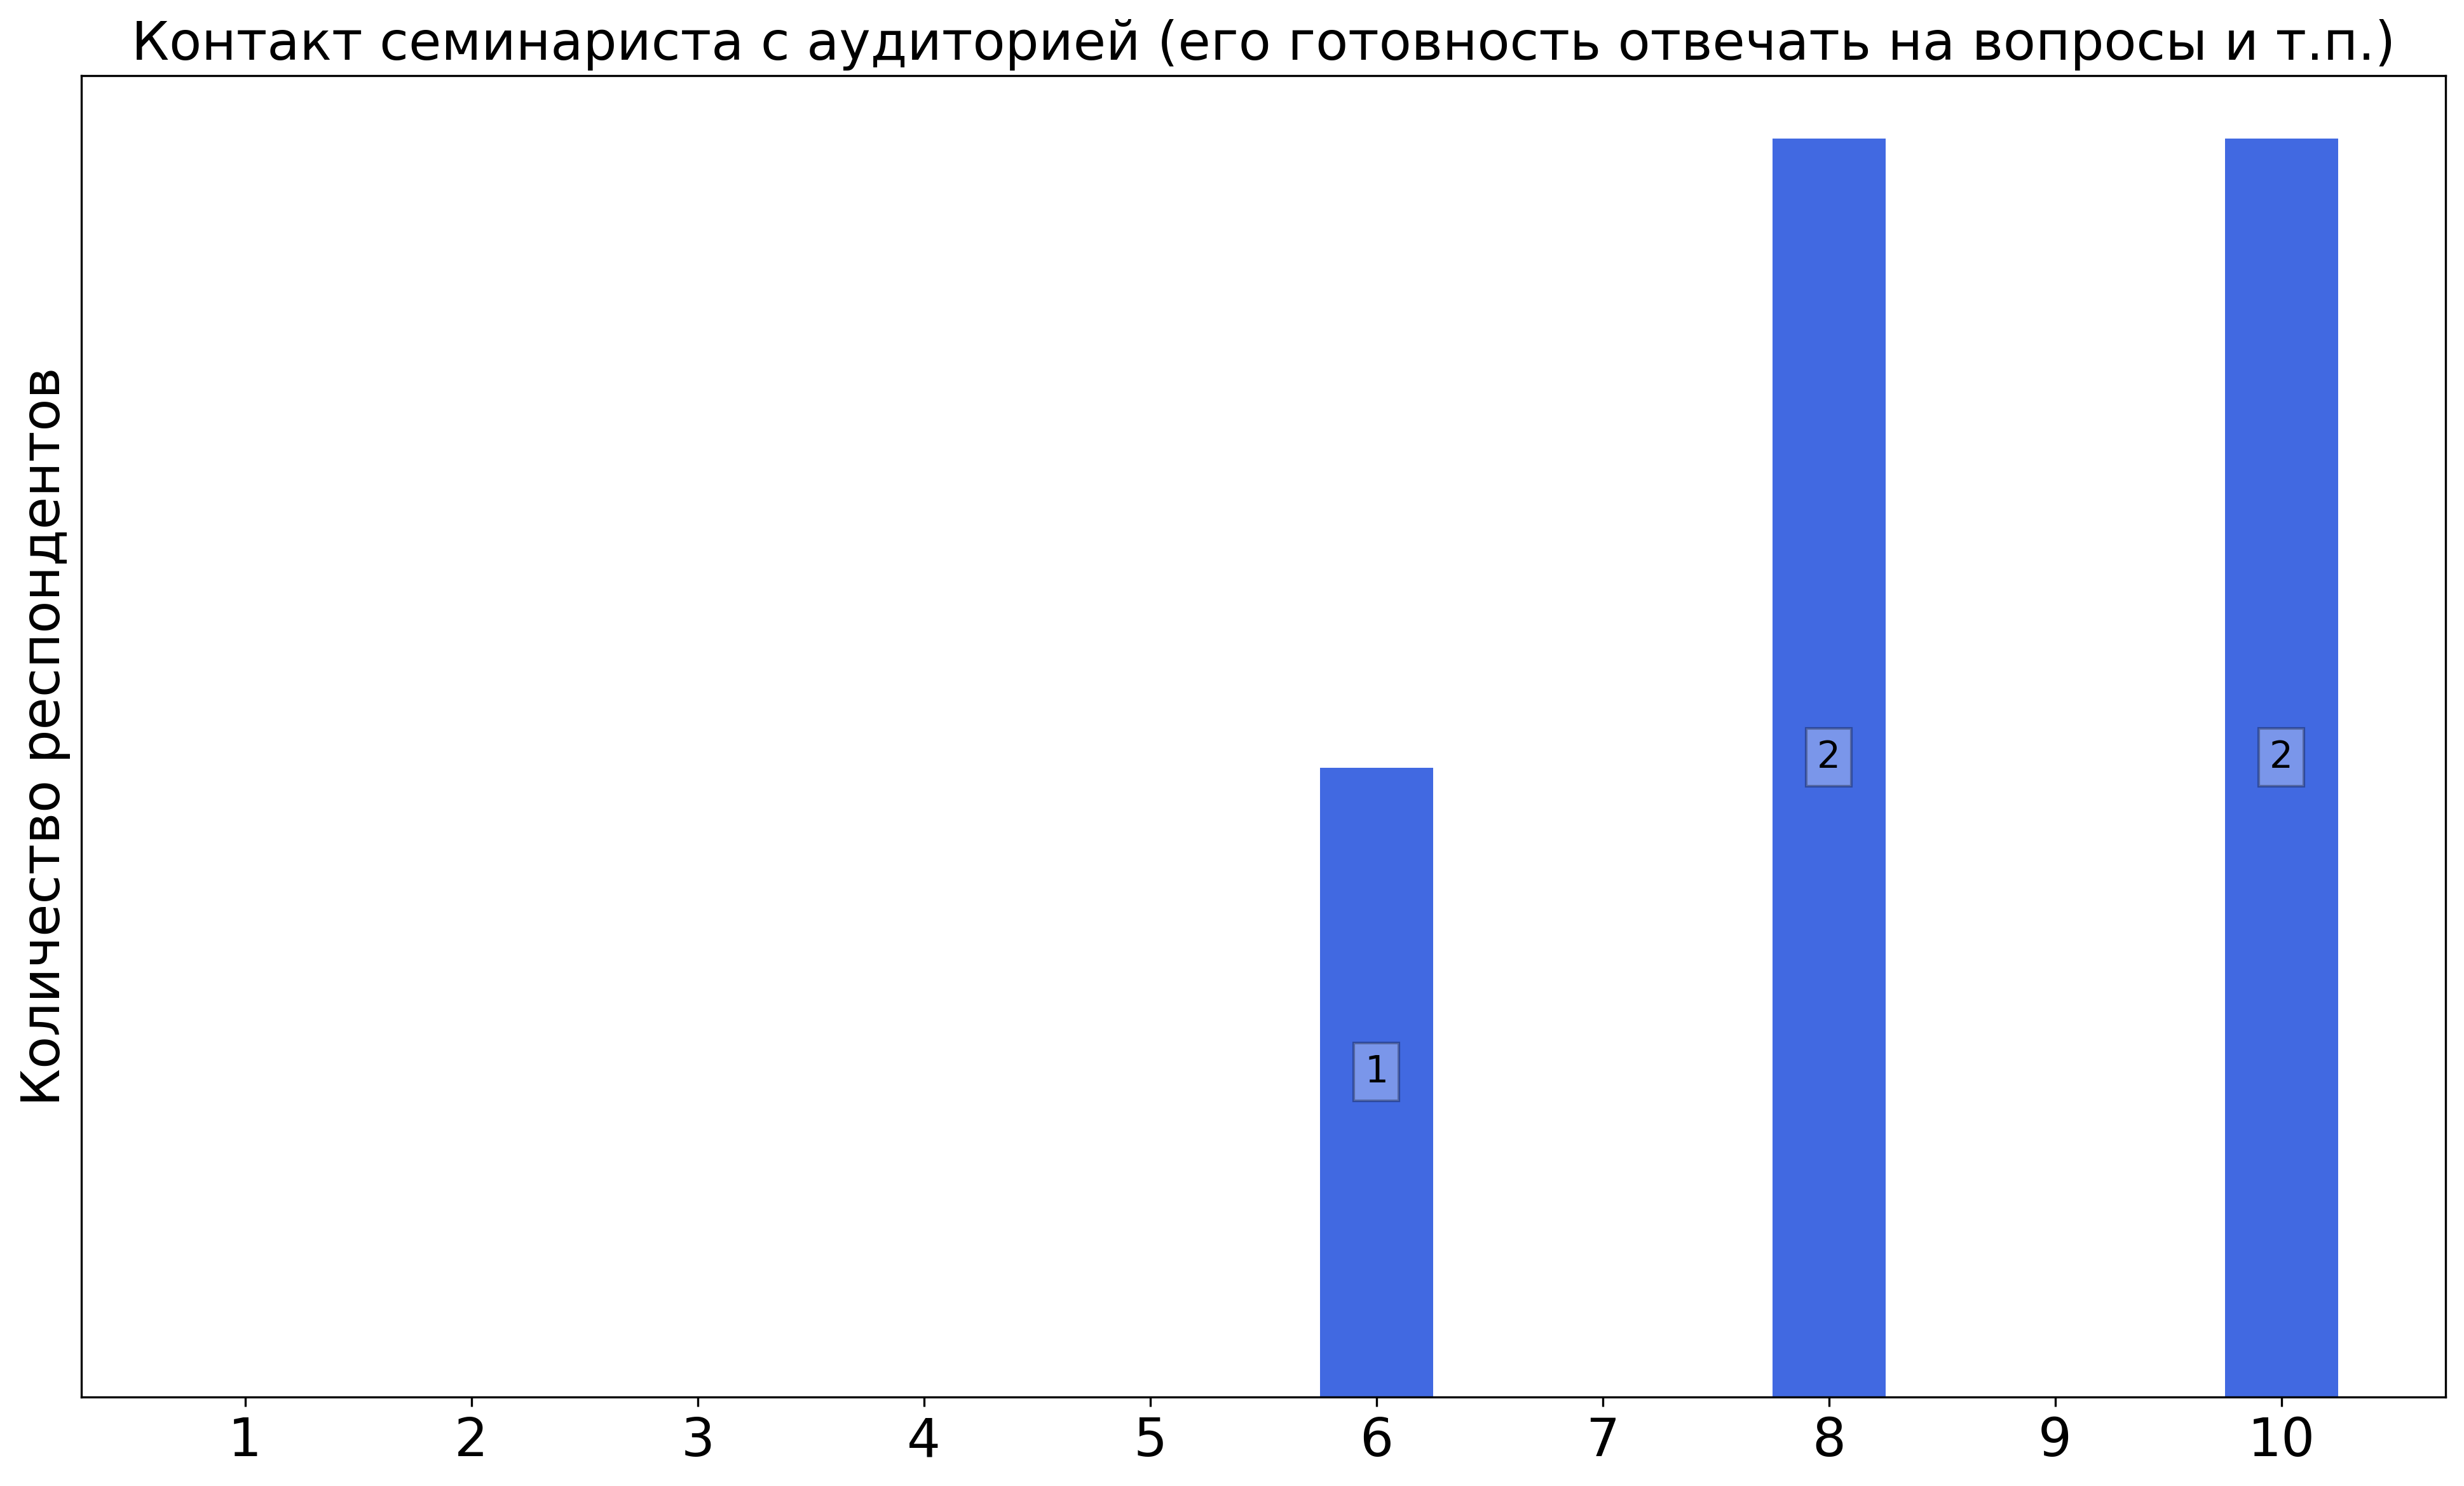
\includegraphics[width=\textwidth]{images/2 course/Компьютерные технологии/seminarists-marks-Красильников Н.И.-0.png}
            \end{subfigure}
            \begin{subfigure}[b]{0.45\textwidth}
                \centering
                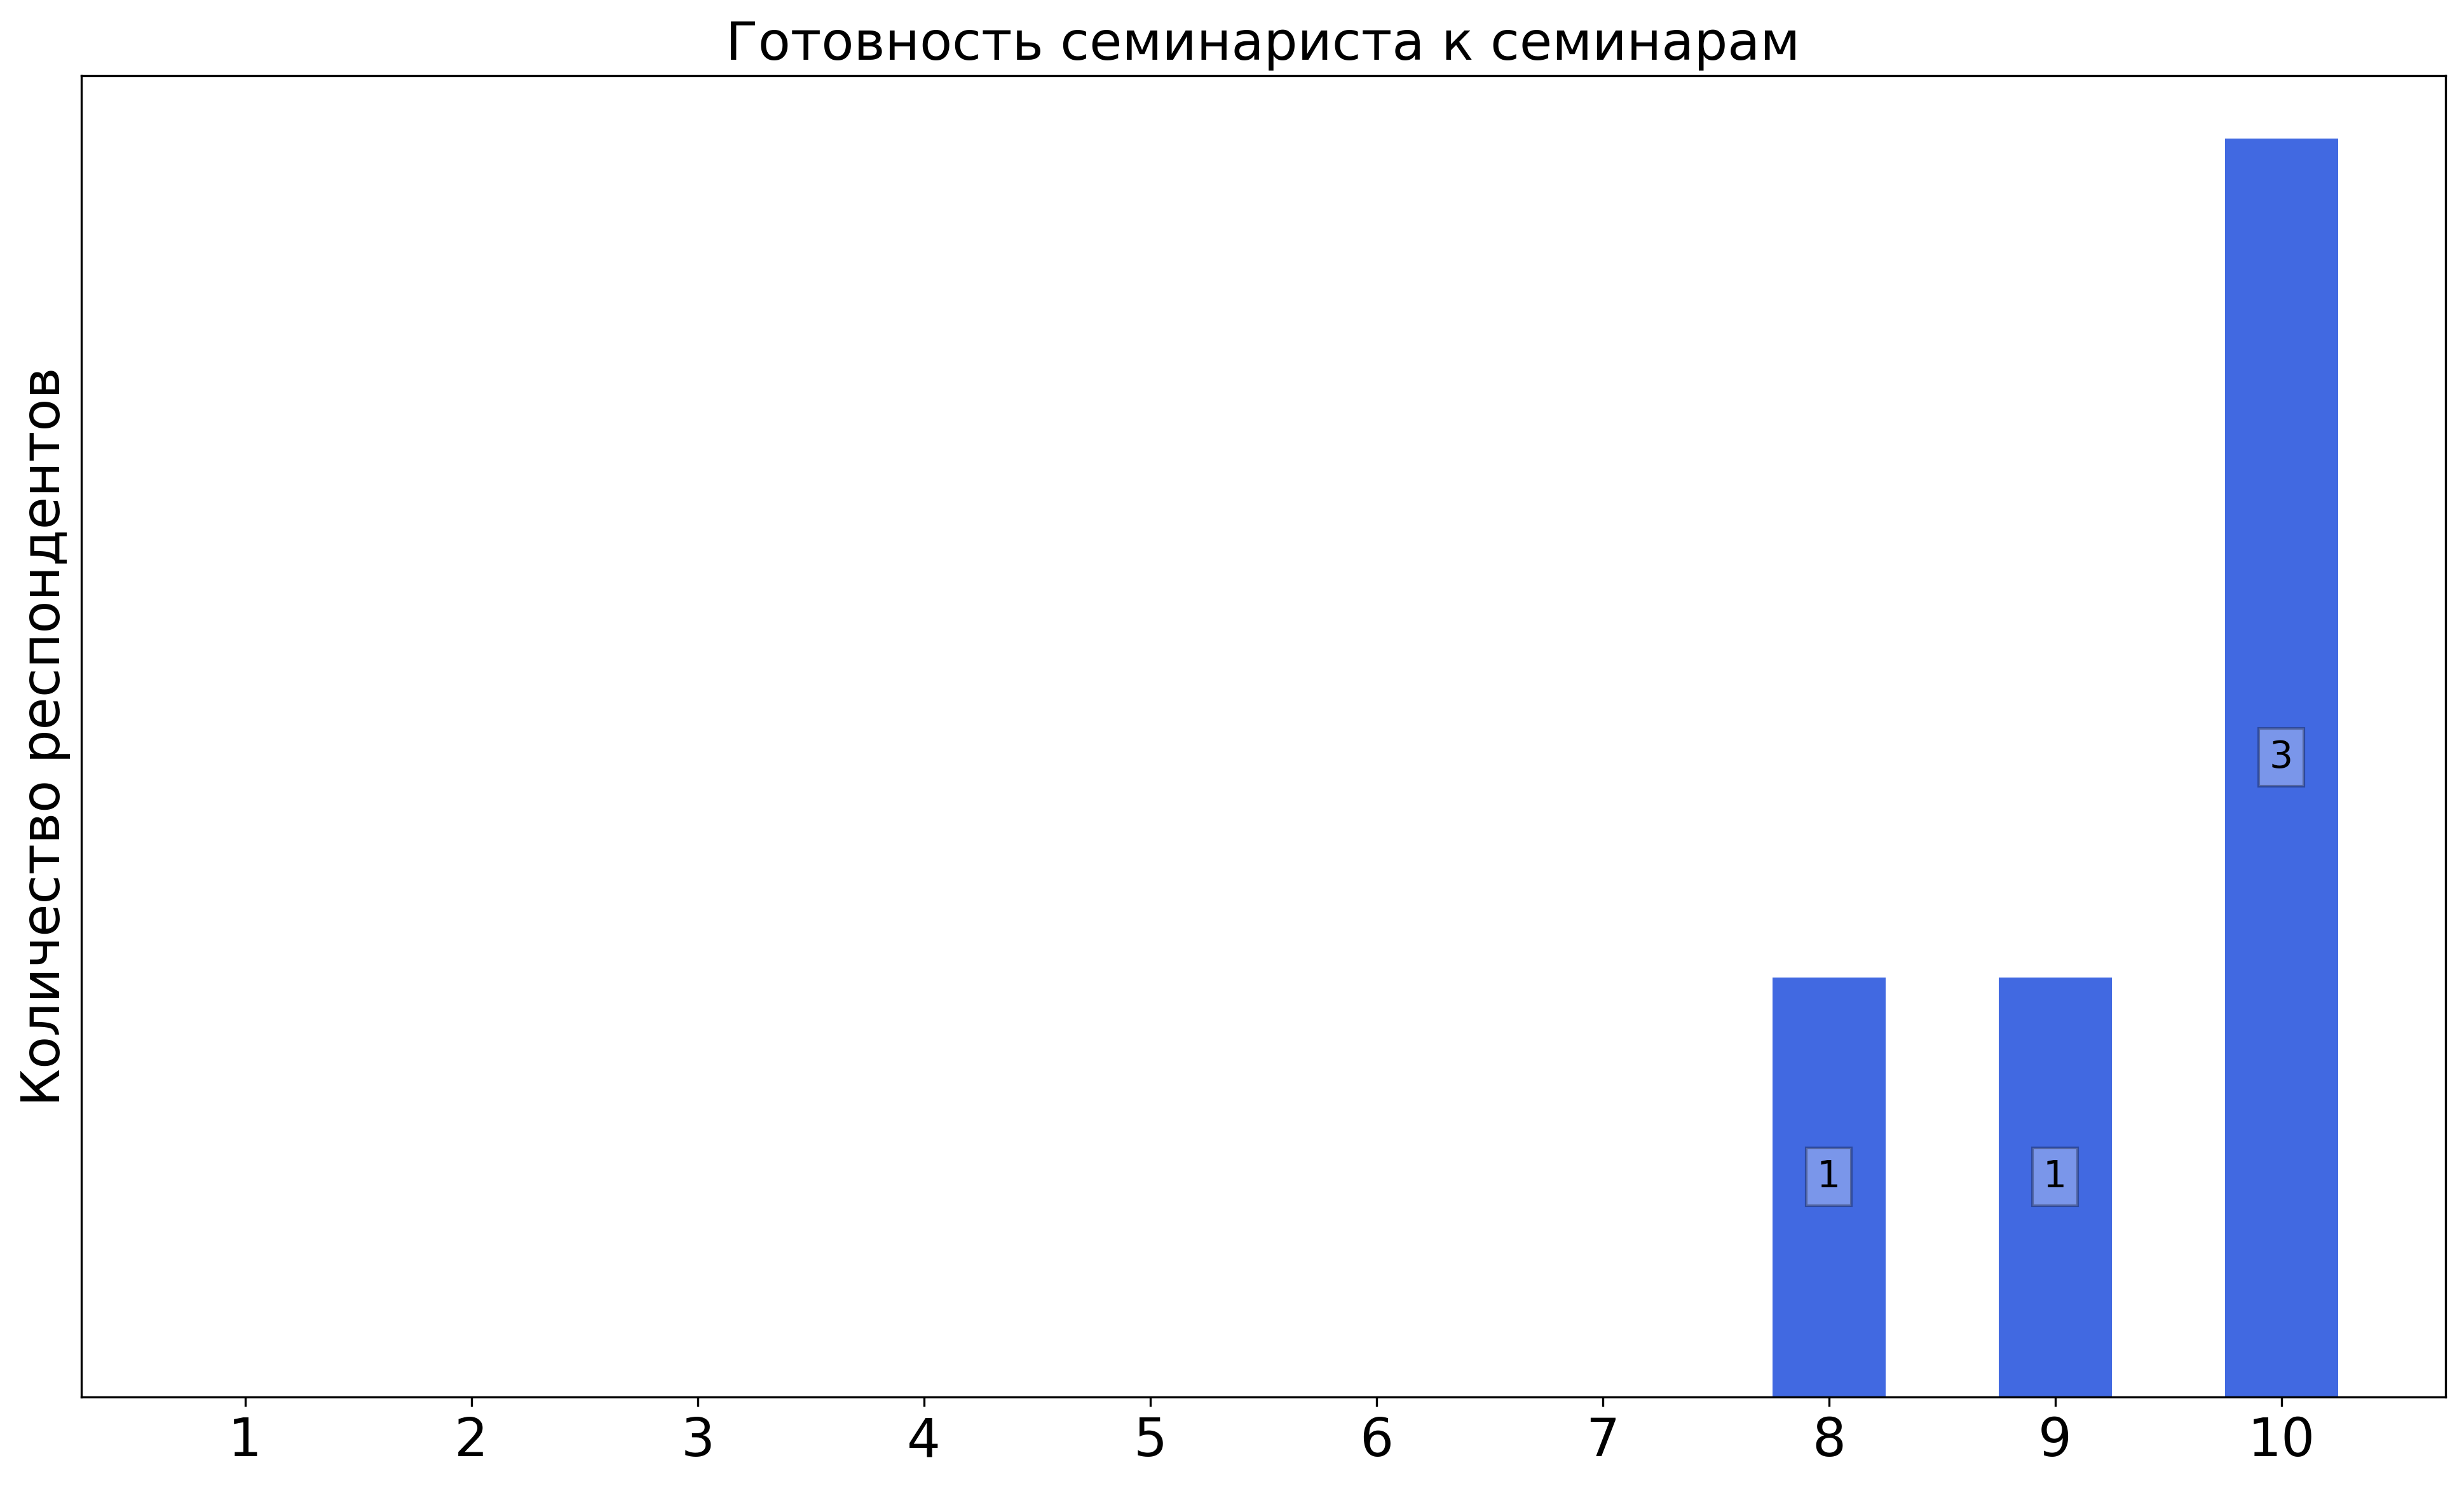
\includegraphics[width=\textwidth]{images/2 course/Компьютерные технологии/seminarists-marks-Красильников Н.И.-1.png}
            \end{subfigure}
            \begin{subfigure}[b]{0.45\textwidth}
                \centering
                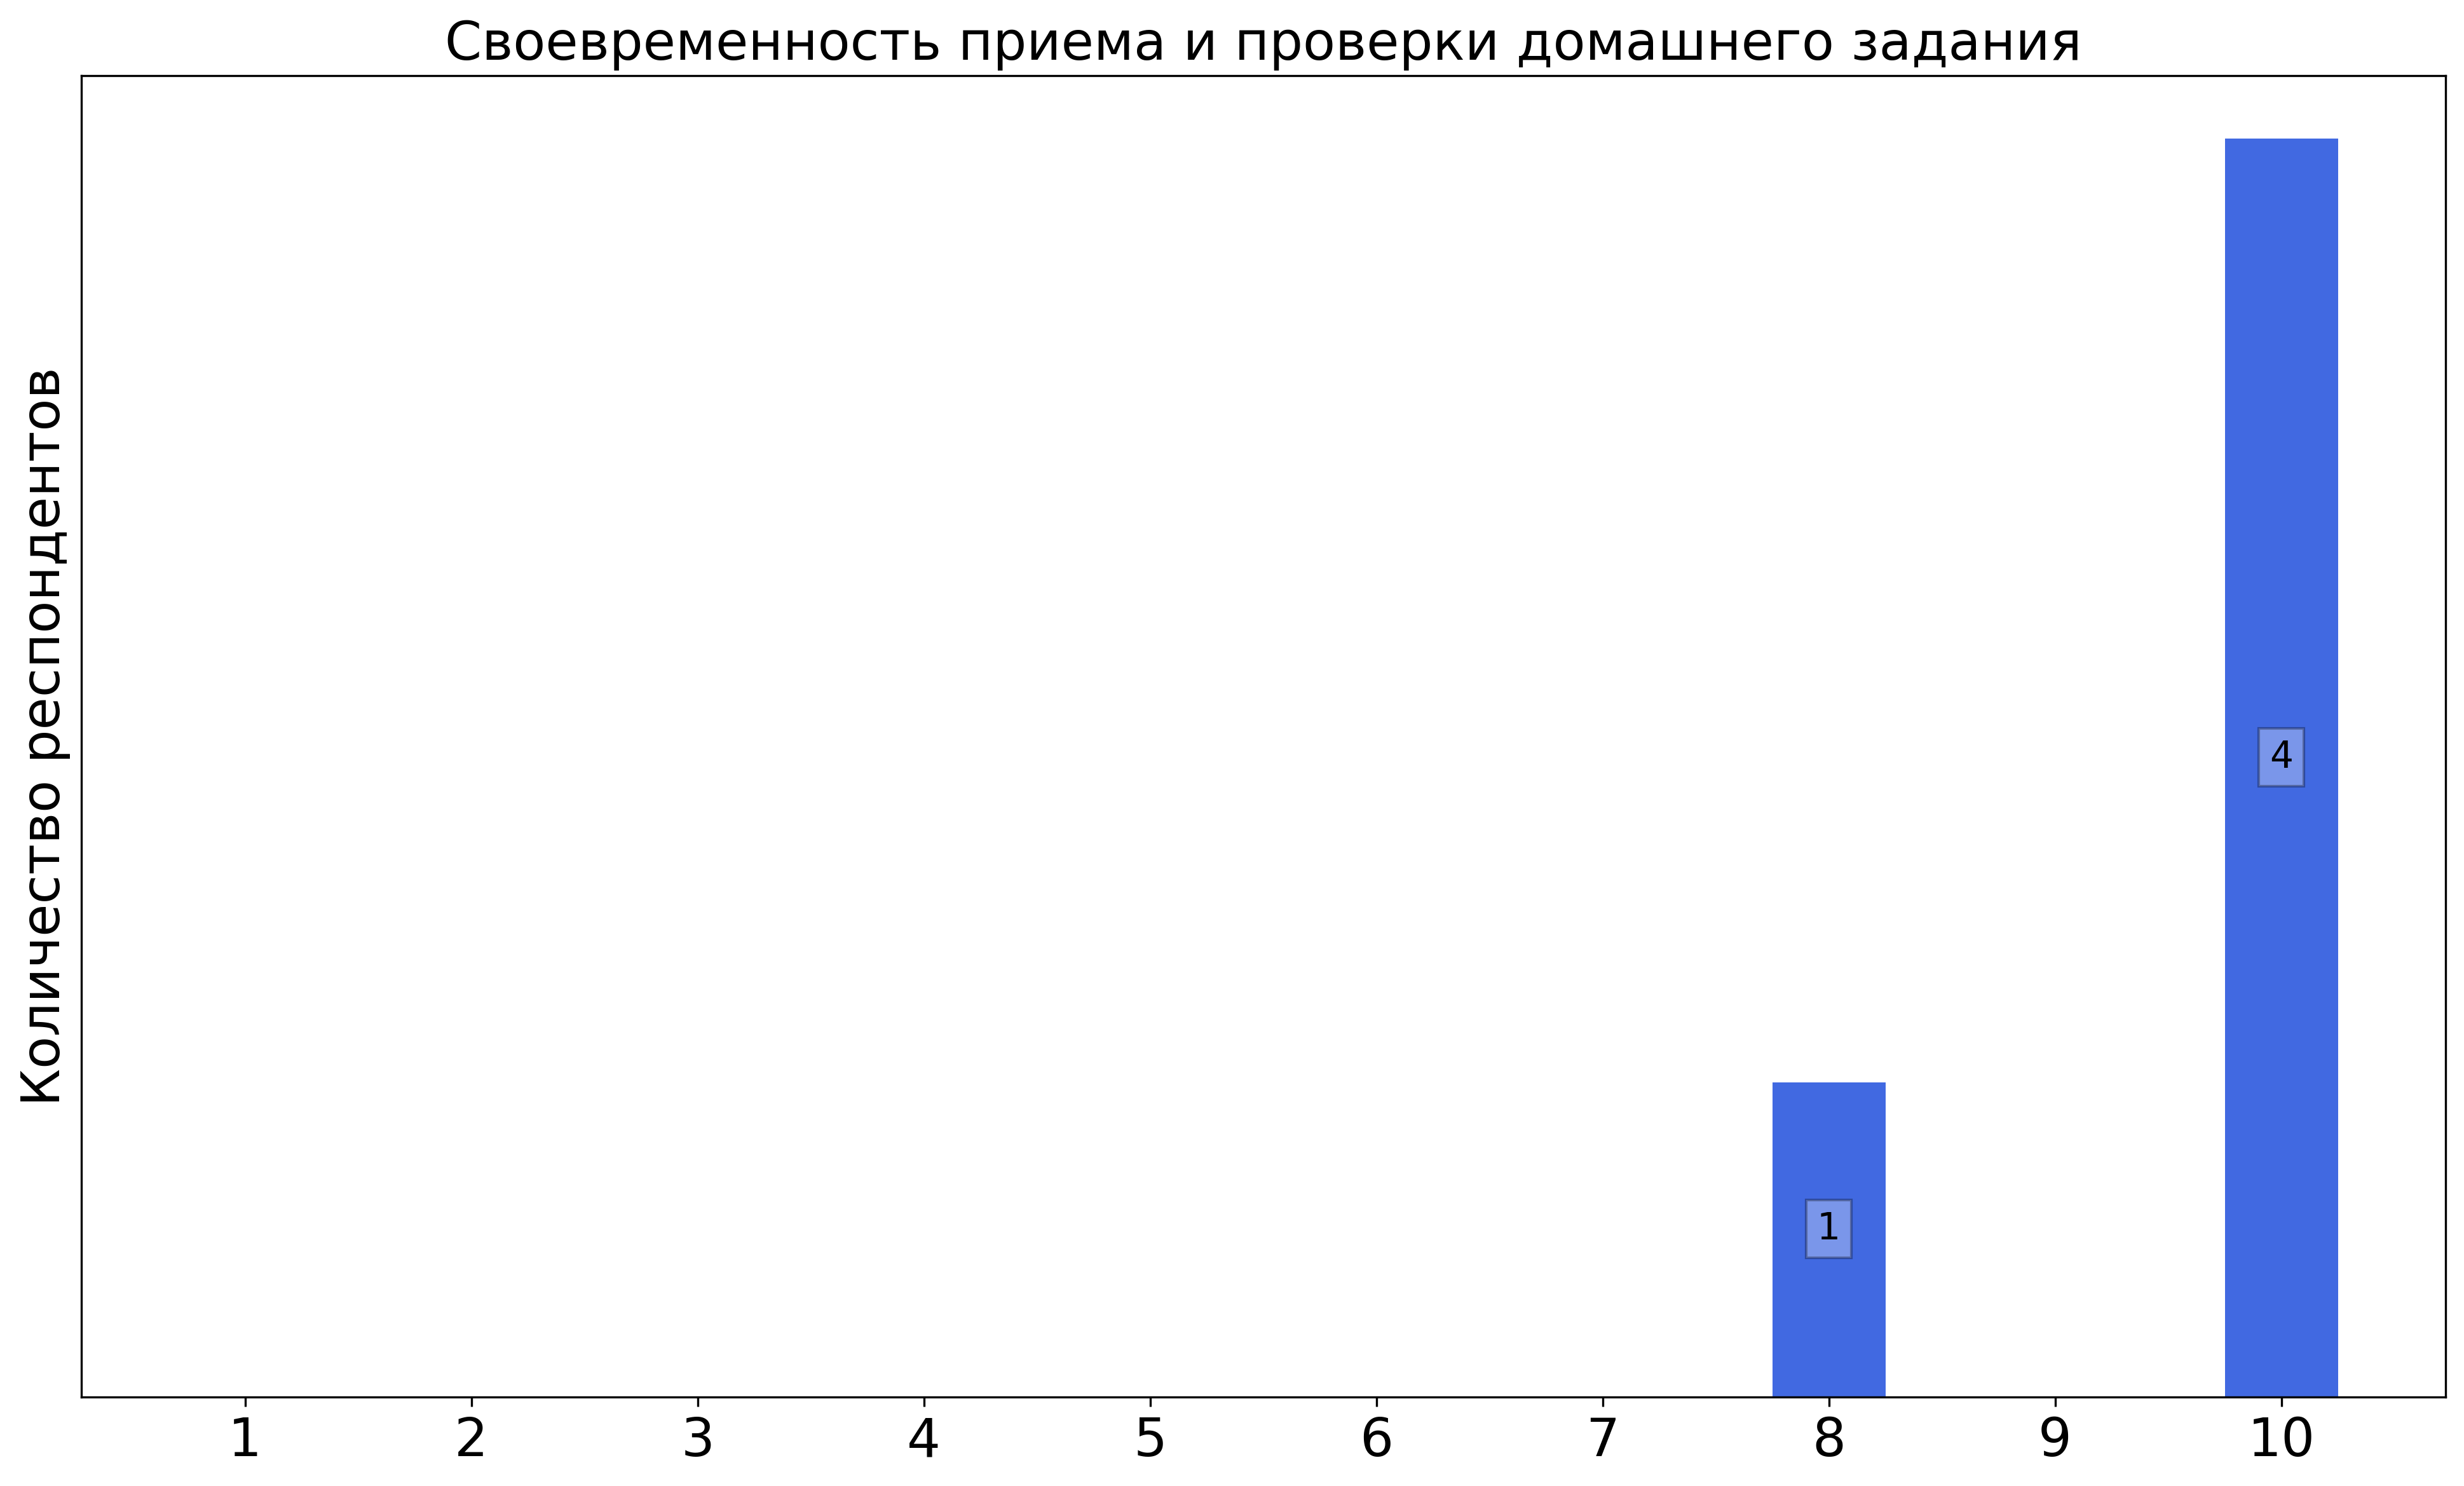
\includegraphics[width=\textwidth]{images/2 course/Компьютерные технологии/seminarists-marks-Красильников Н.И.-2.png}
            \end{subfigure}
            \begin{subfigure}[b]{0.45\textwidth}
                \centering
                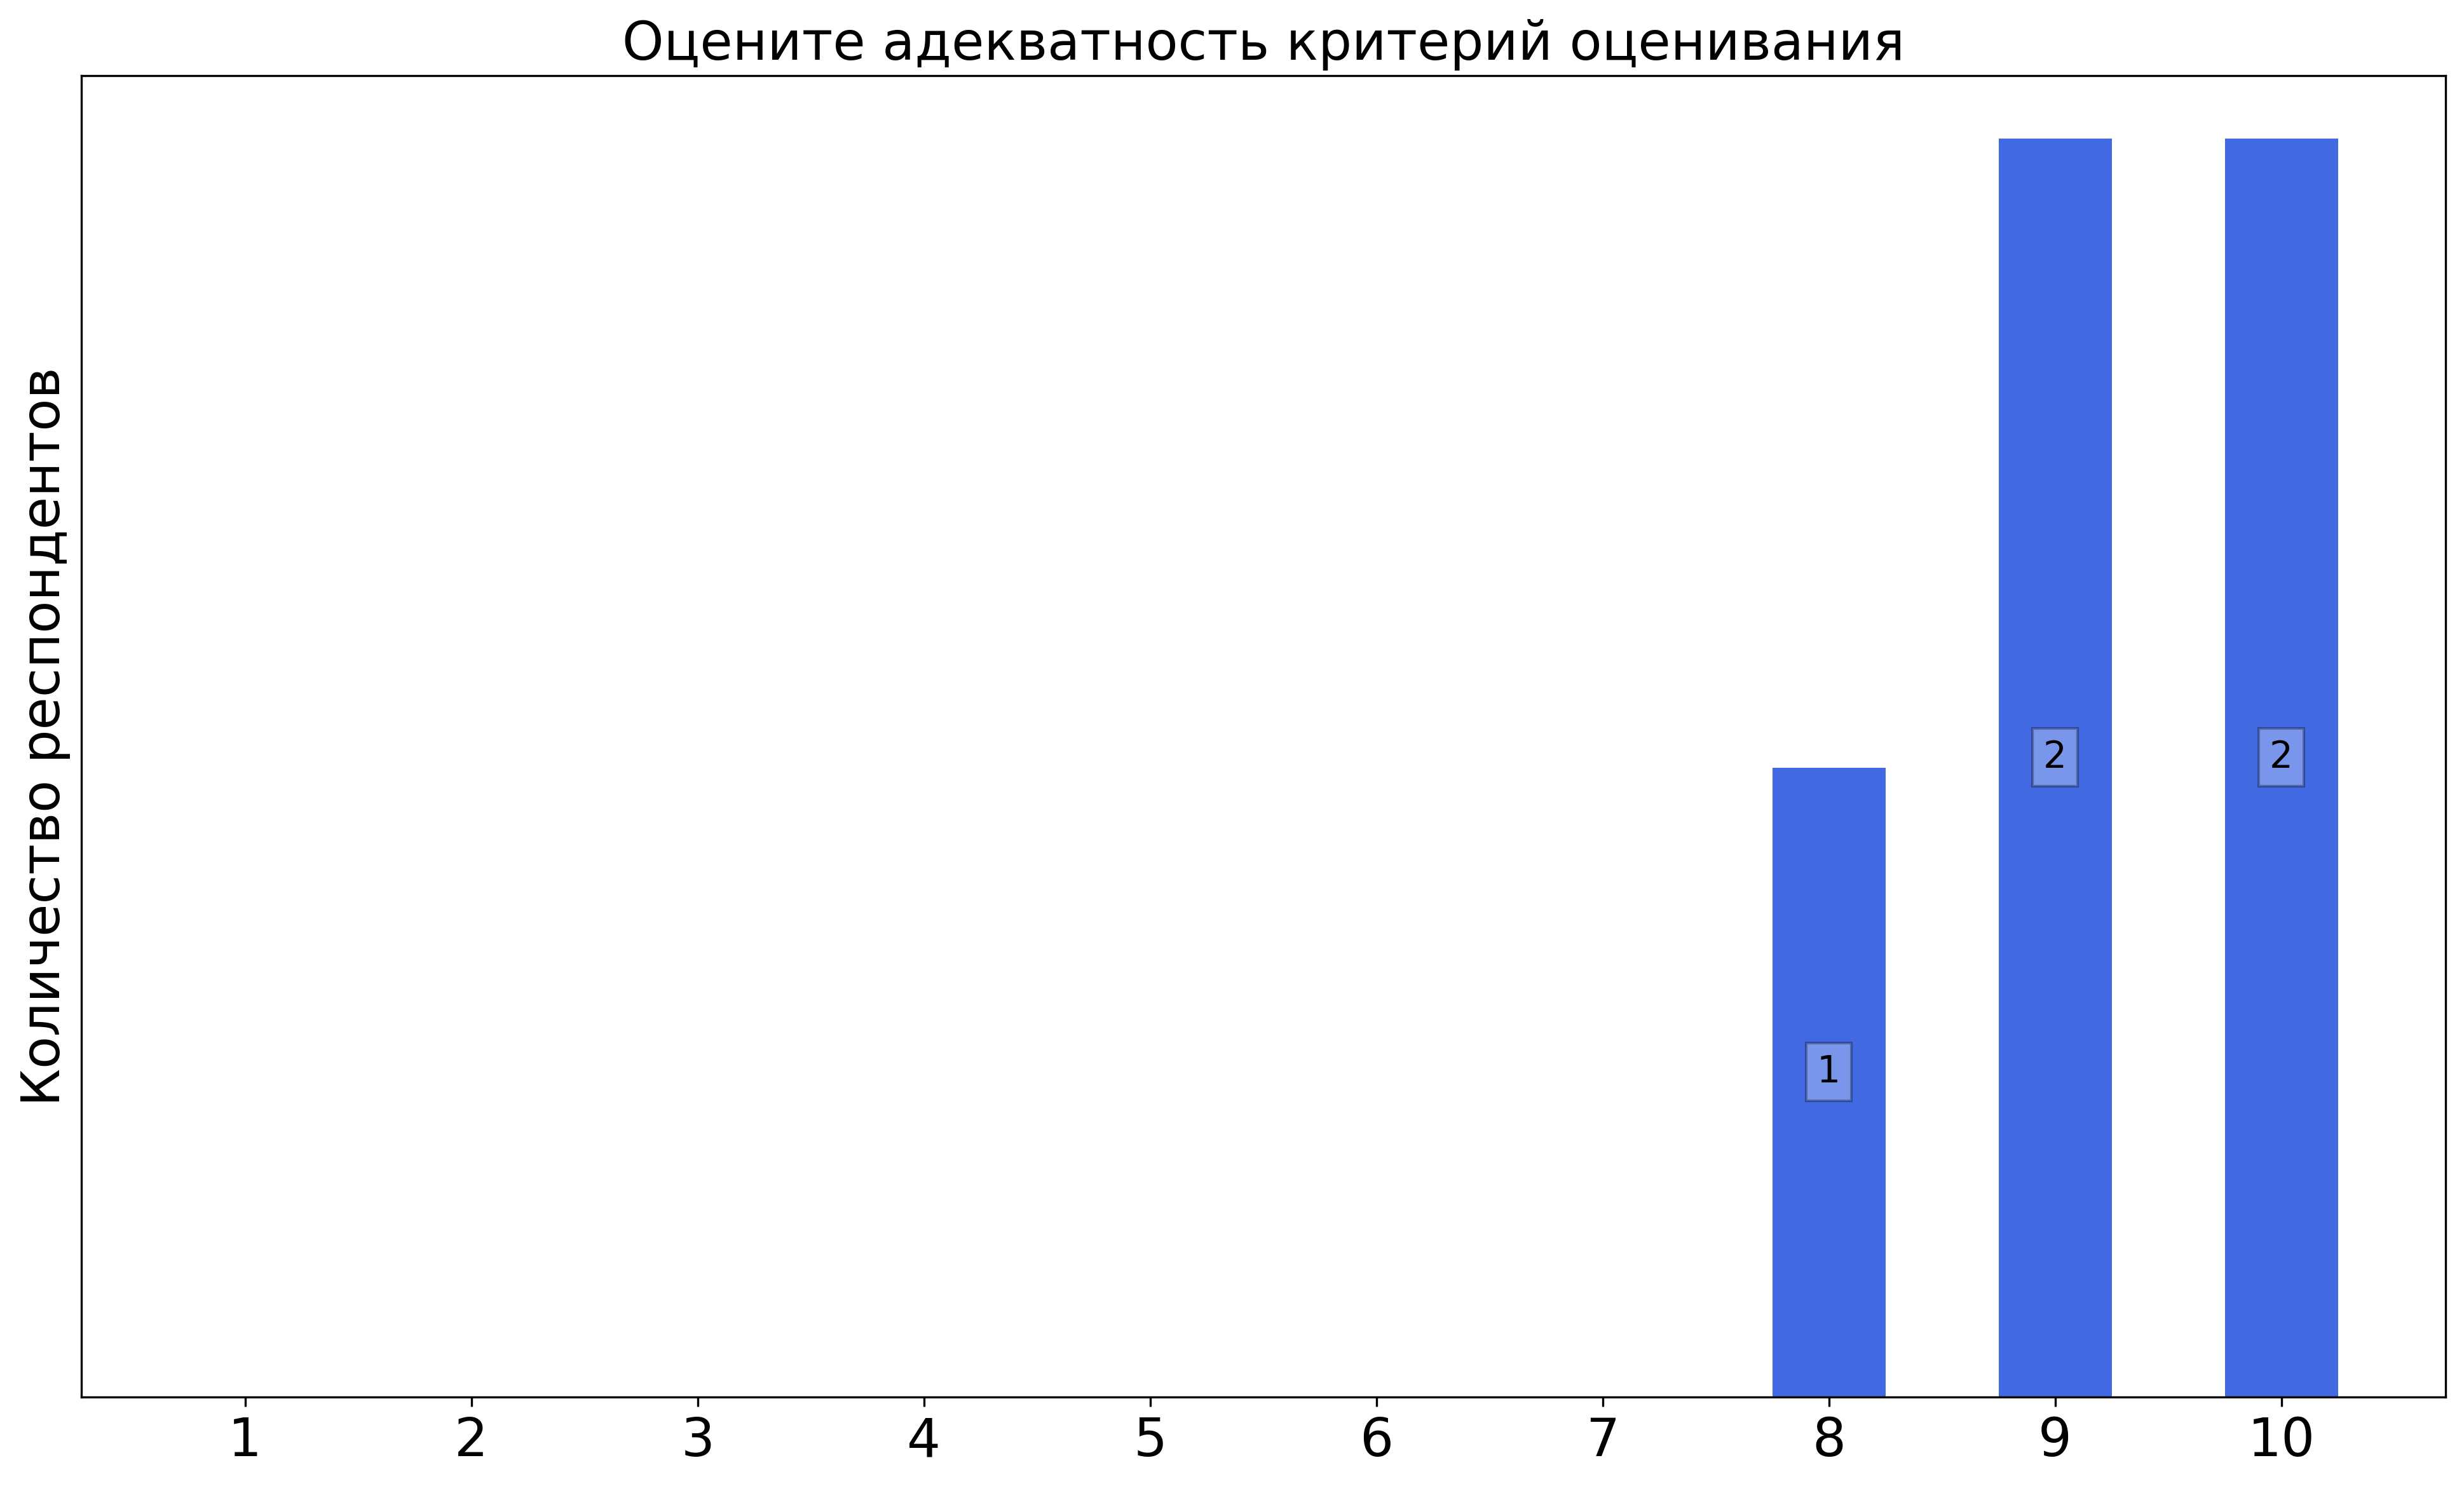
\includegraphics[width=\textwidth]{images/2 course/Компьютерные технологии/seminarists-marks-Красильников Н.И.-3.png}
            \end{subfigure}	
            \caption{Оценки респондентов о качестве преподавания семинаров}
        \end{figure}

        \textbf{Комментарии студентов о семинаристе\protect\footnote{сохранены оригинальные орфография и пунктуация}}
            \begin{commentbox} 
                единственный случай, когда на любой вопрос "читайте книгу"- неиронично хороший ответ: после нескольких чтений Карпова кое-как понимаешь, где и почему что-то не работает 
            \end{commentbox}


    
    \subsubsection{Отзыв студентов о семинарах. Семинарист: Кулиев Р.С.}
        \begin{figure}[H]
            \centering
            \begin{subfigure}[b]{0.45\textwidth}
                \centering
                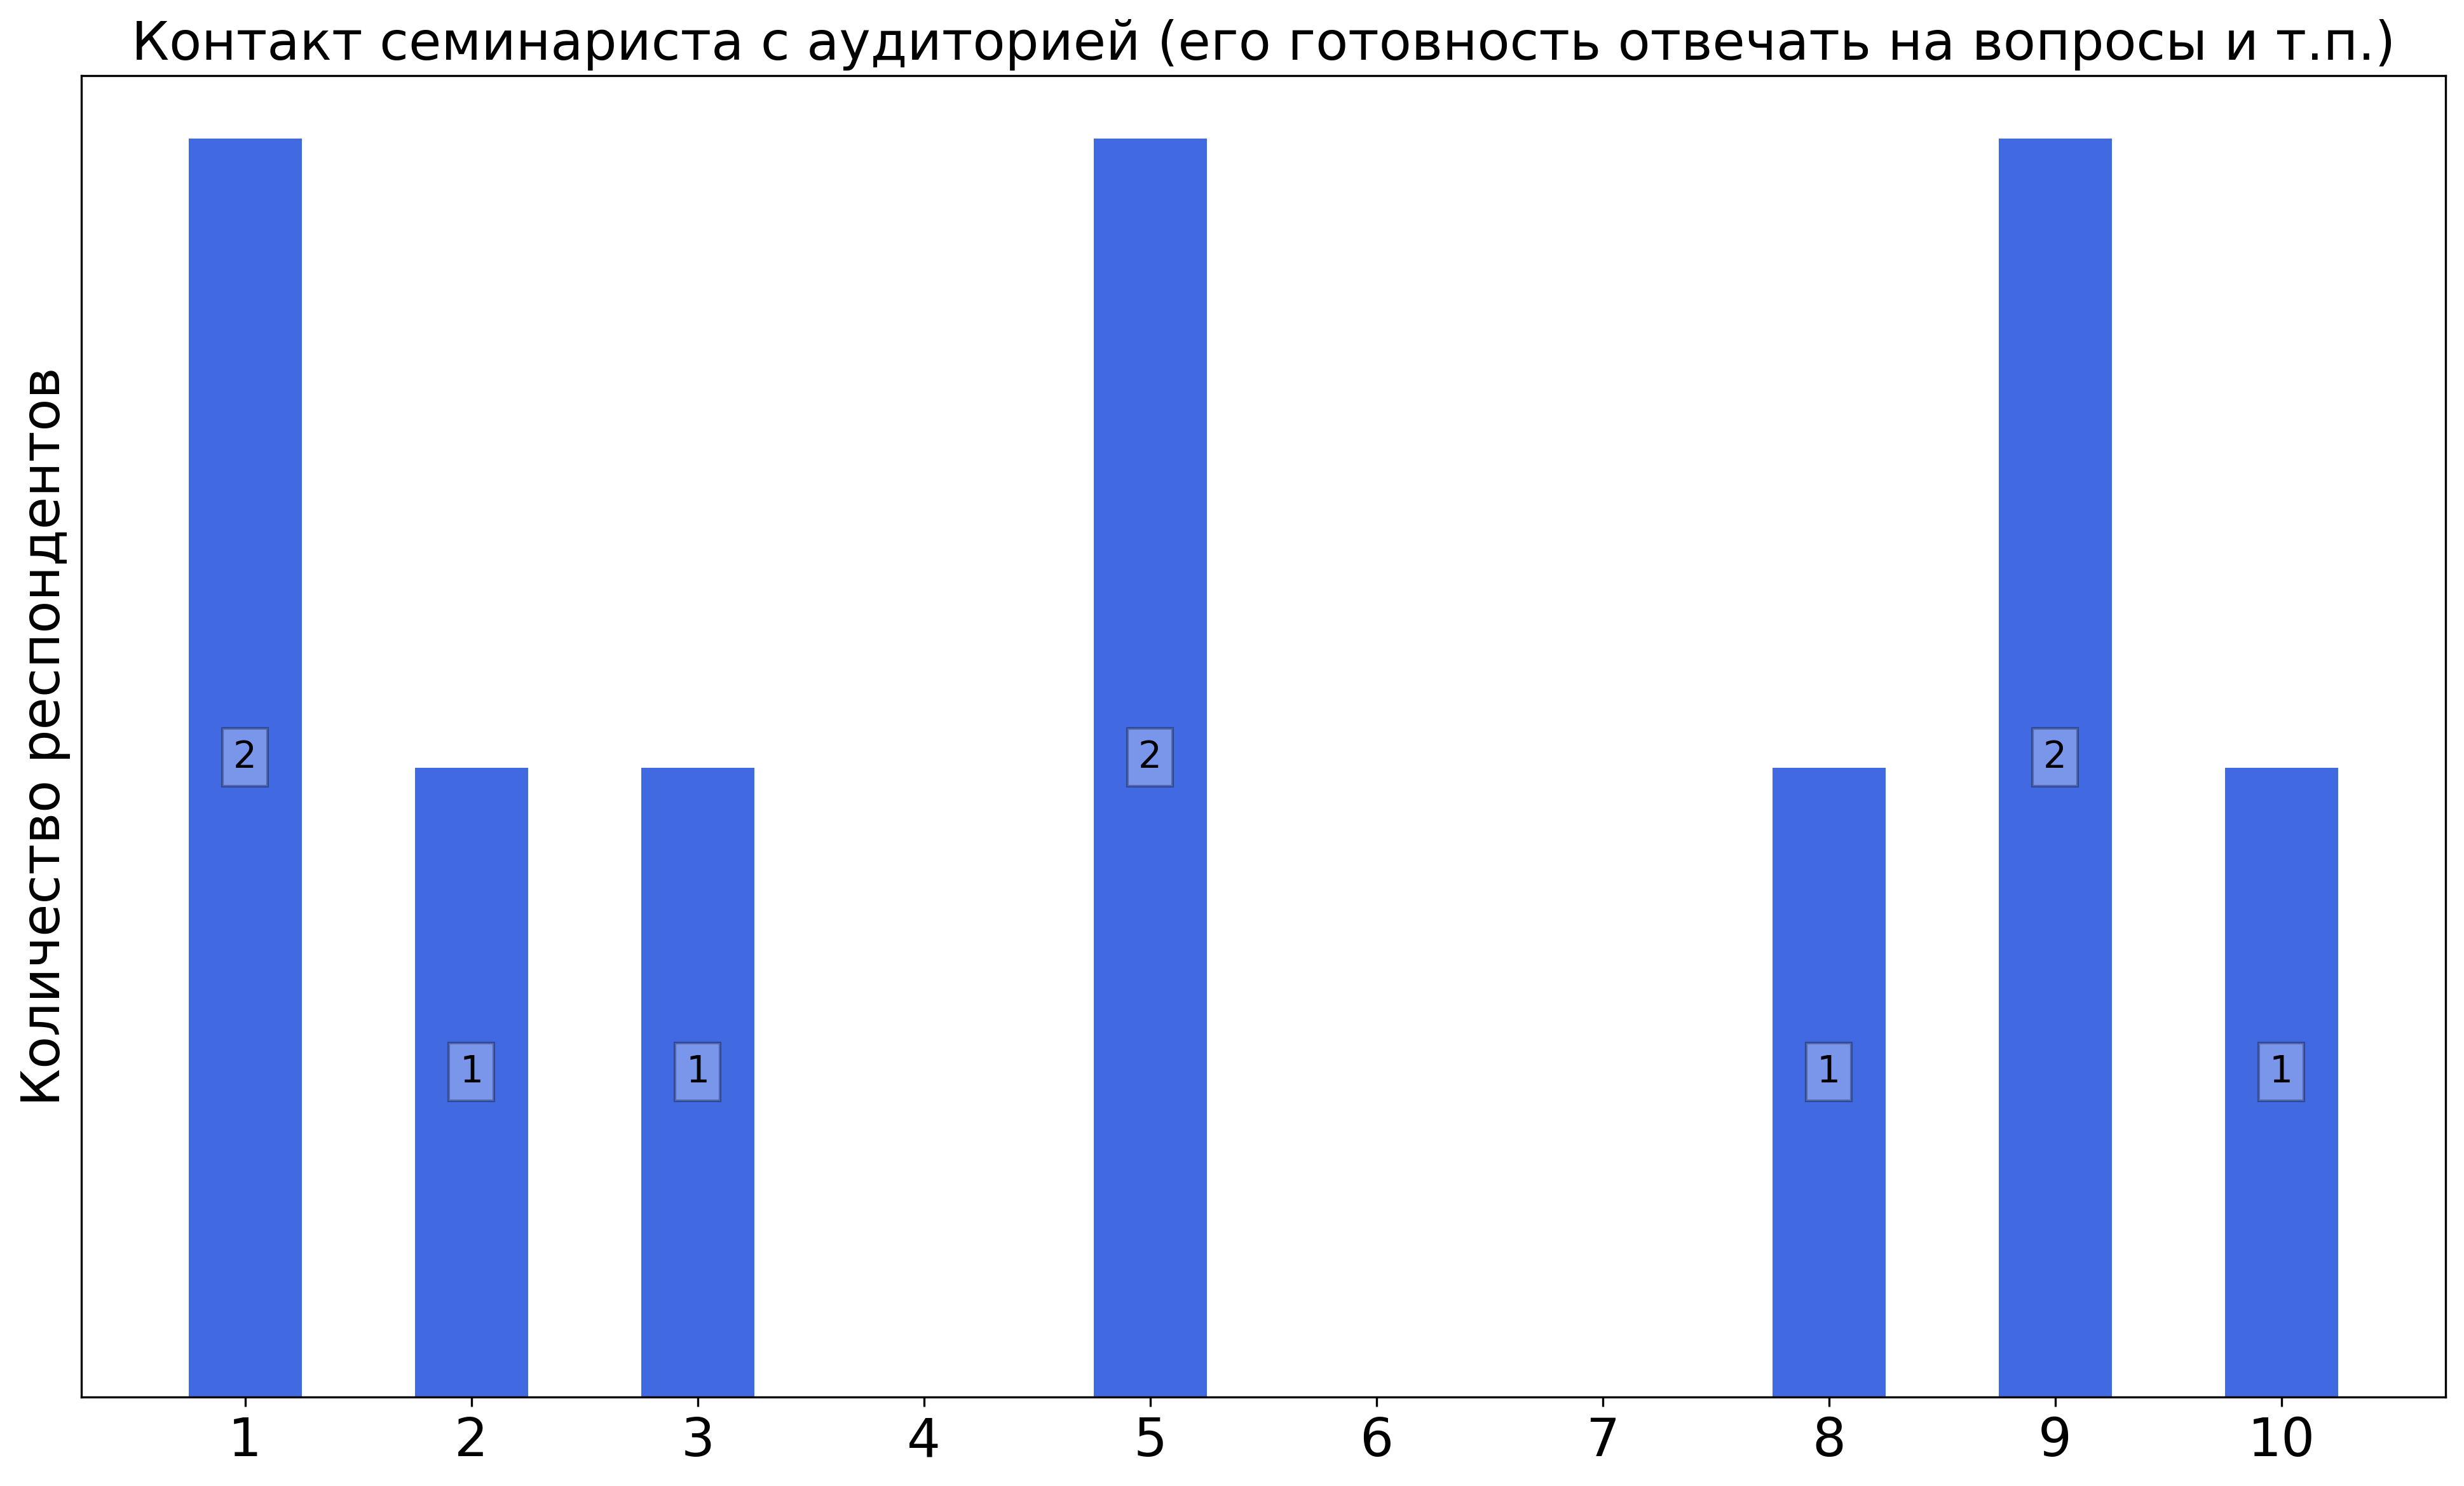
\includegraphics[width=\textwidth]{images/2 course/Компьютерные технологии/seminarists-marks-Кулиев Р.С.-0.png}
            \end{subfigure}
            \begin{subfigure}[b]{0.45\textwidth}
                \centering
                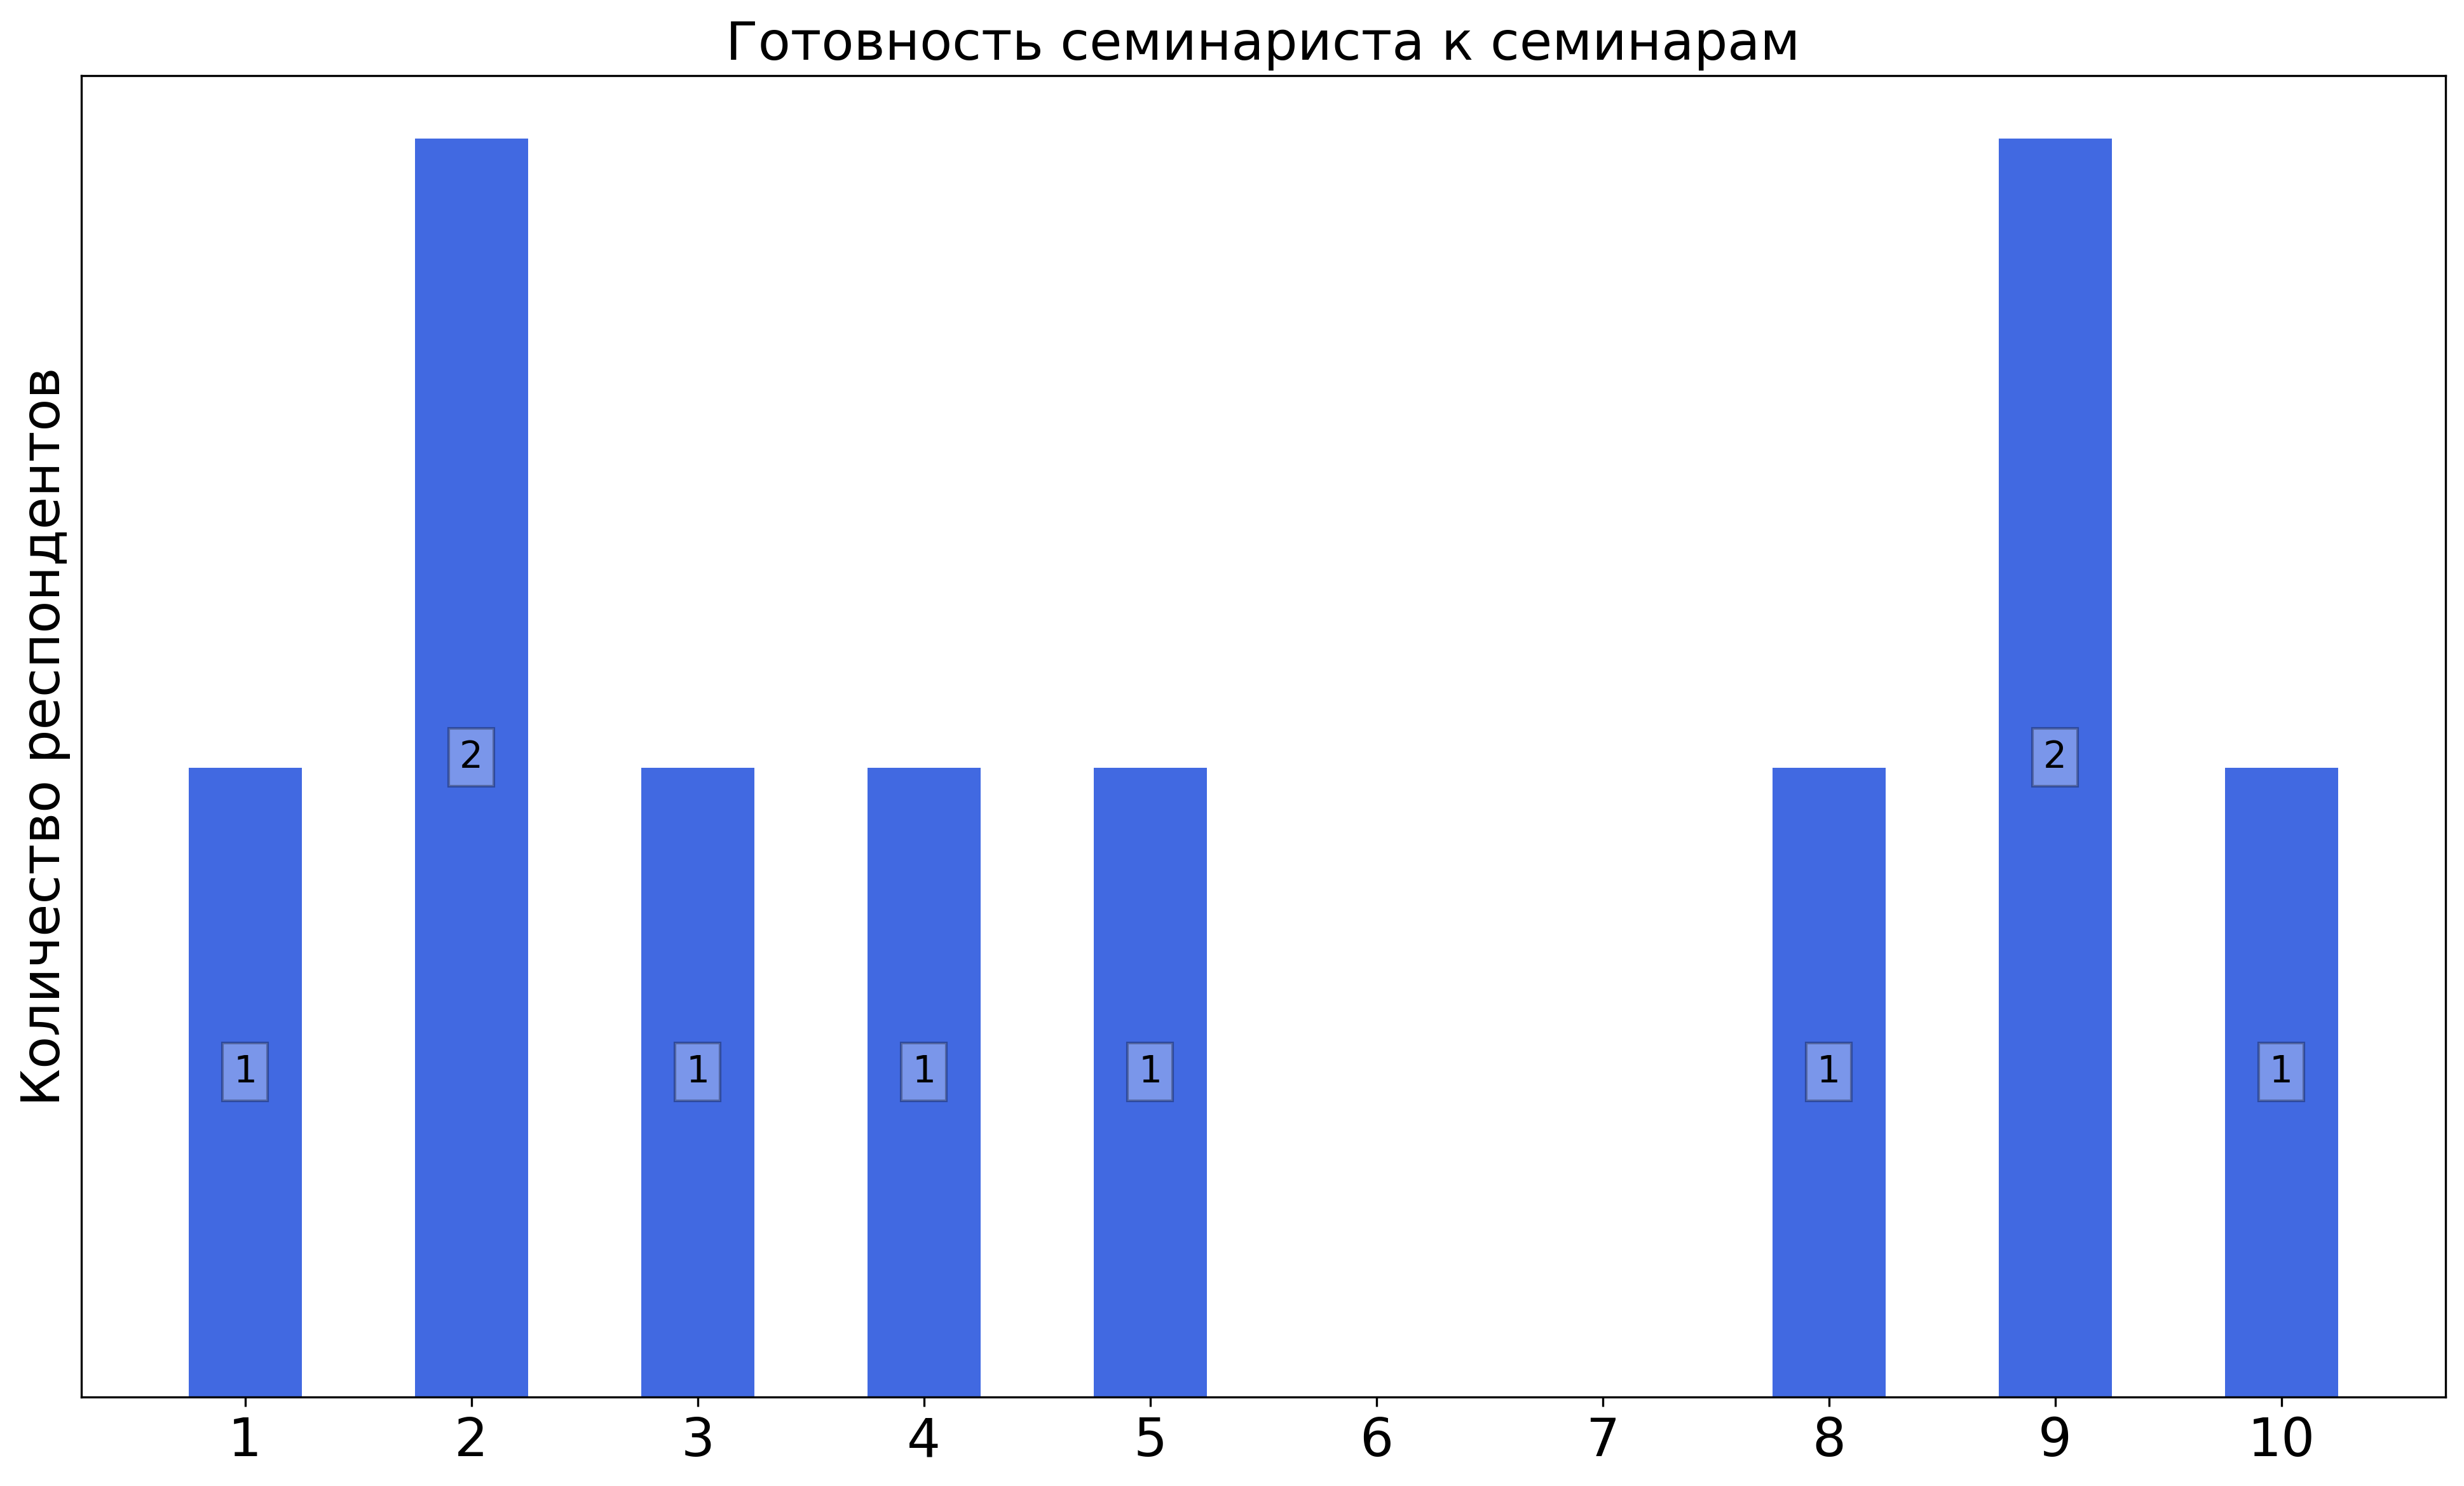
\includegraphics[width=\textwidth]{images/2 course/Компьютерные технологии/seminarists-marks-Кулиев Р.С.-1.png}
            \end{subfigure}
            \begin{subfigure}[b]{0.45\textwidth}
                \centering
                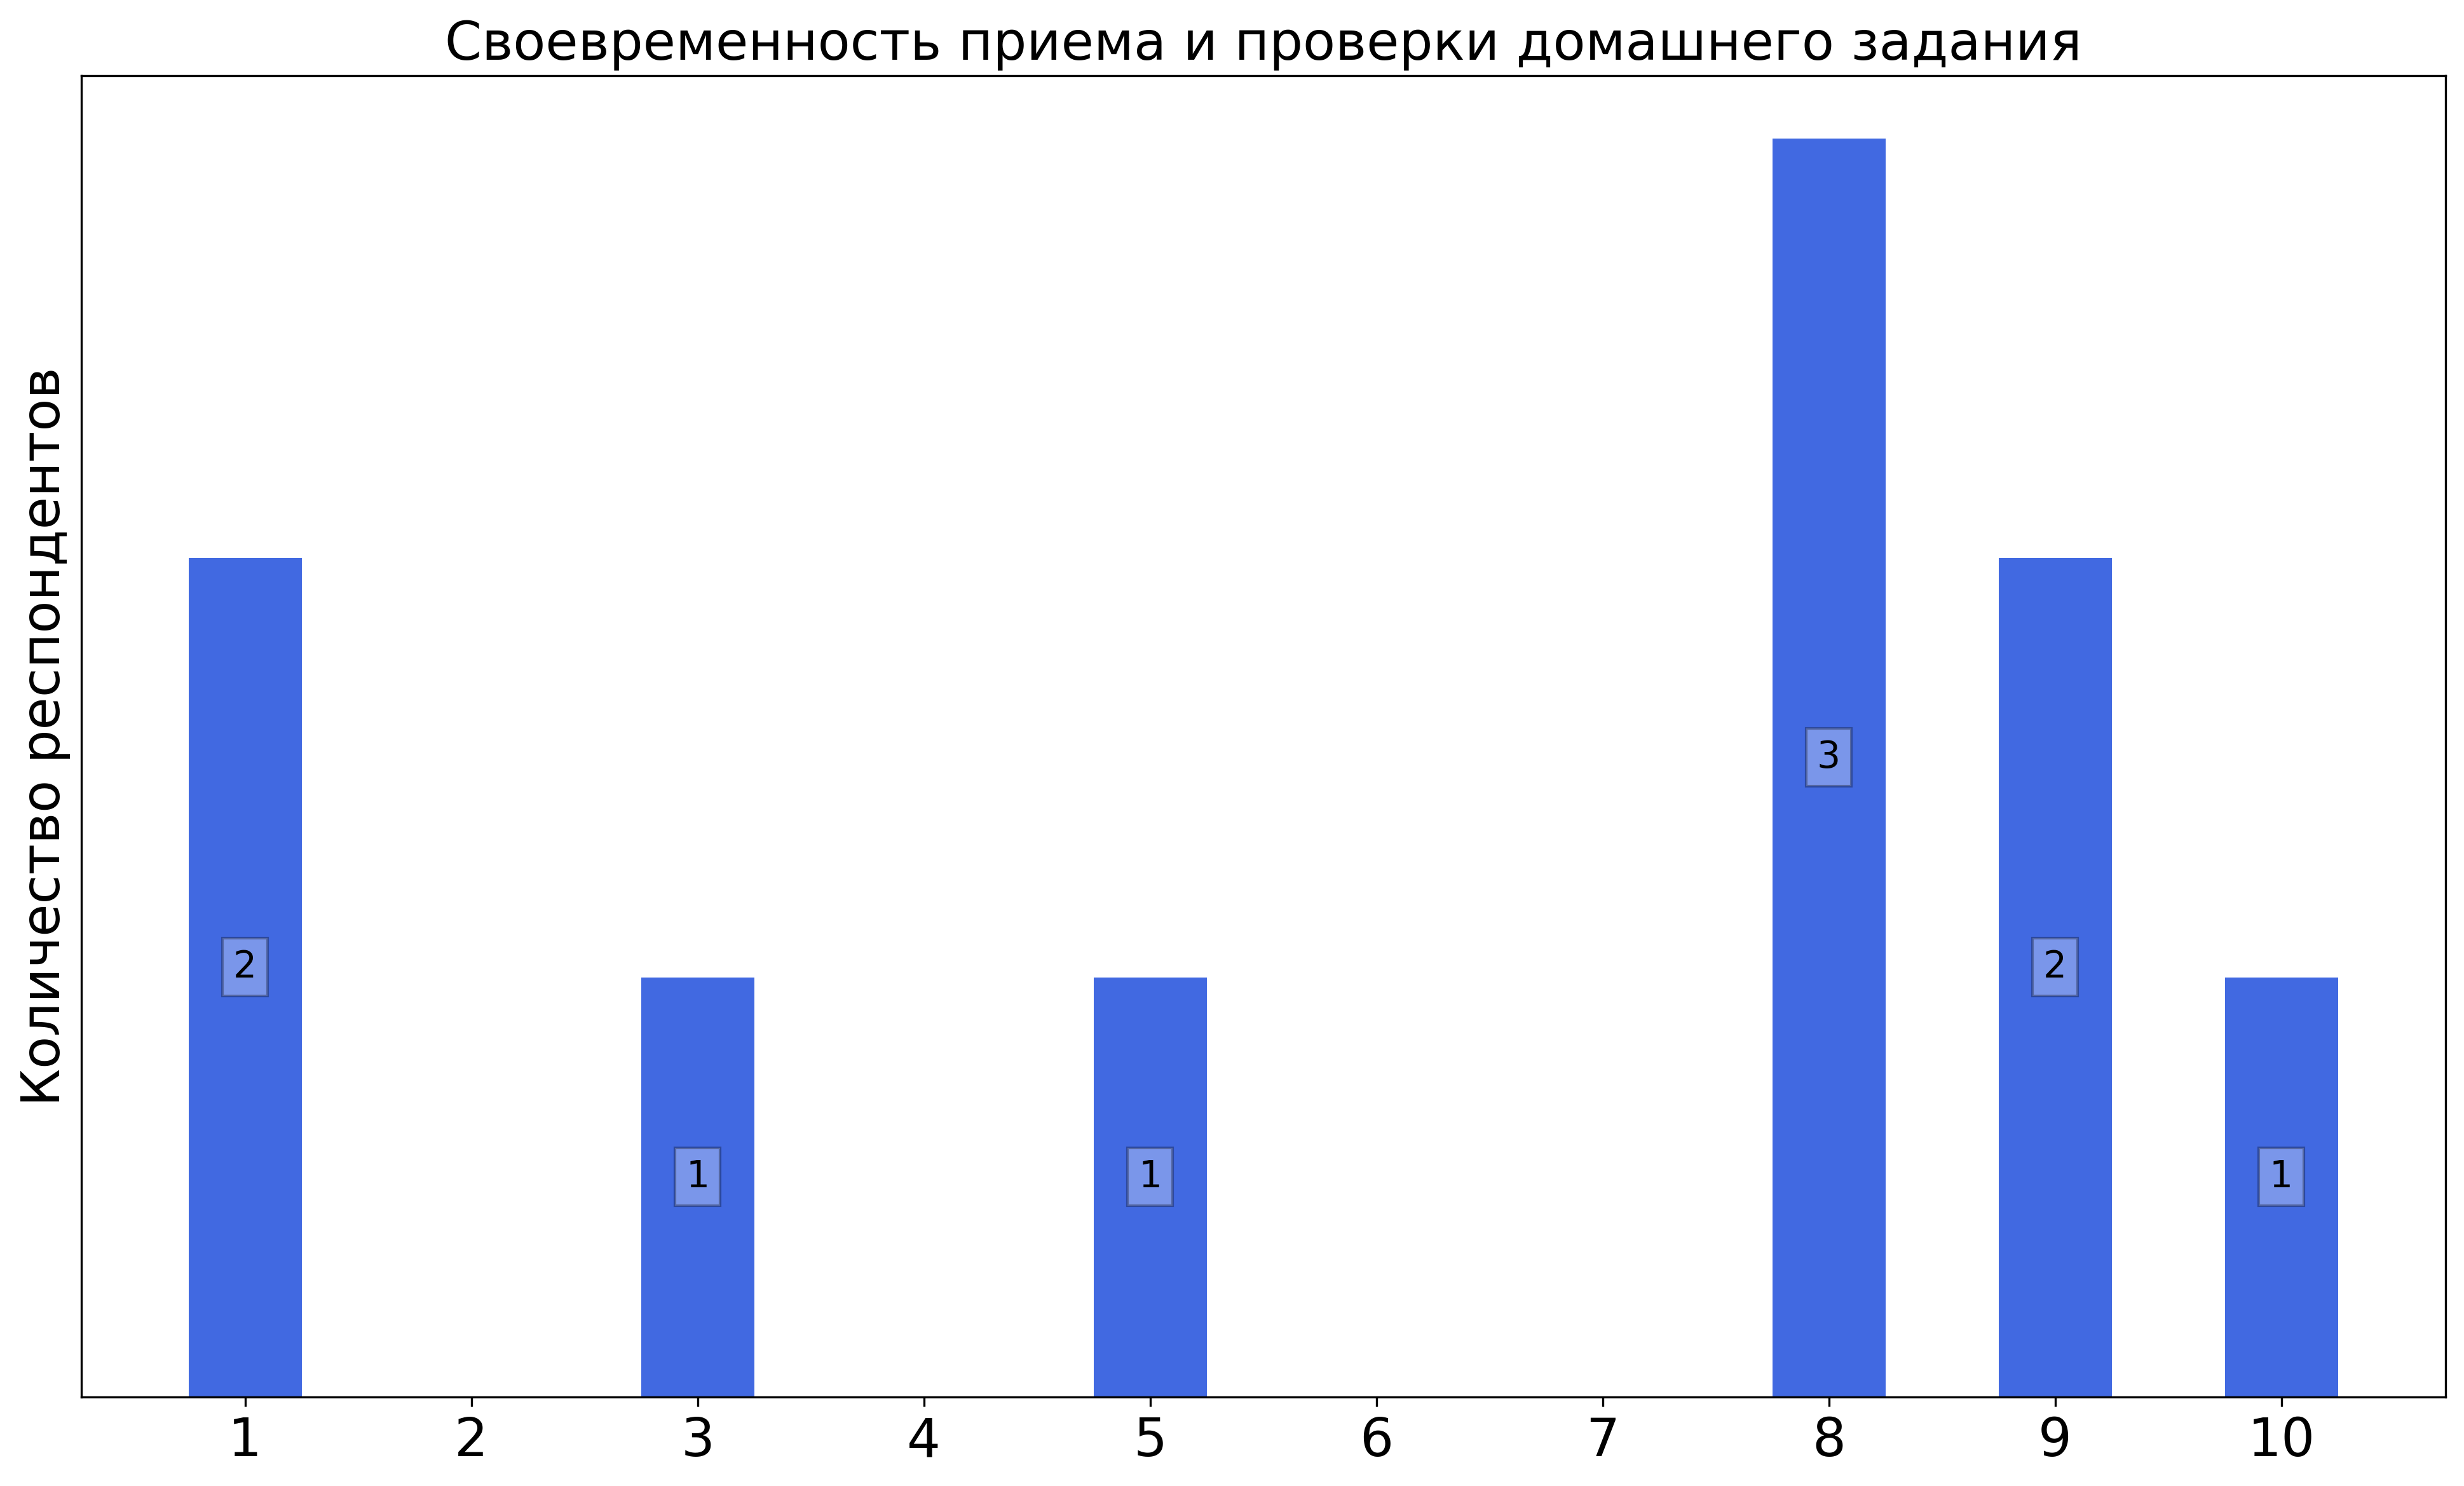
\includegraphics[width=\textwidth]{images/2 course/Компьютерные технологии/seminarists-marks-Кулиев Р.С.-2.png}
            \end{subfigure}
            \begin{subfigure}[b]{0.45\textwidth}
                \centering
                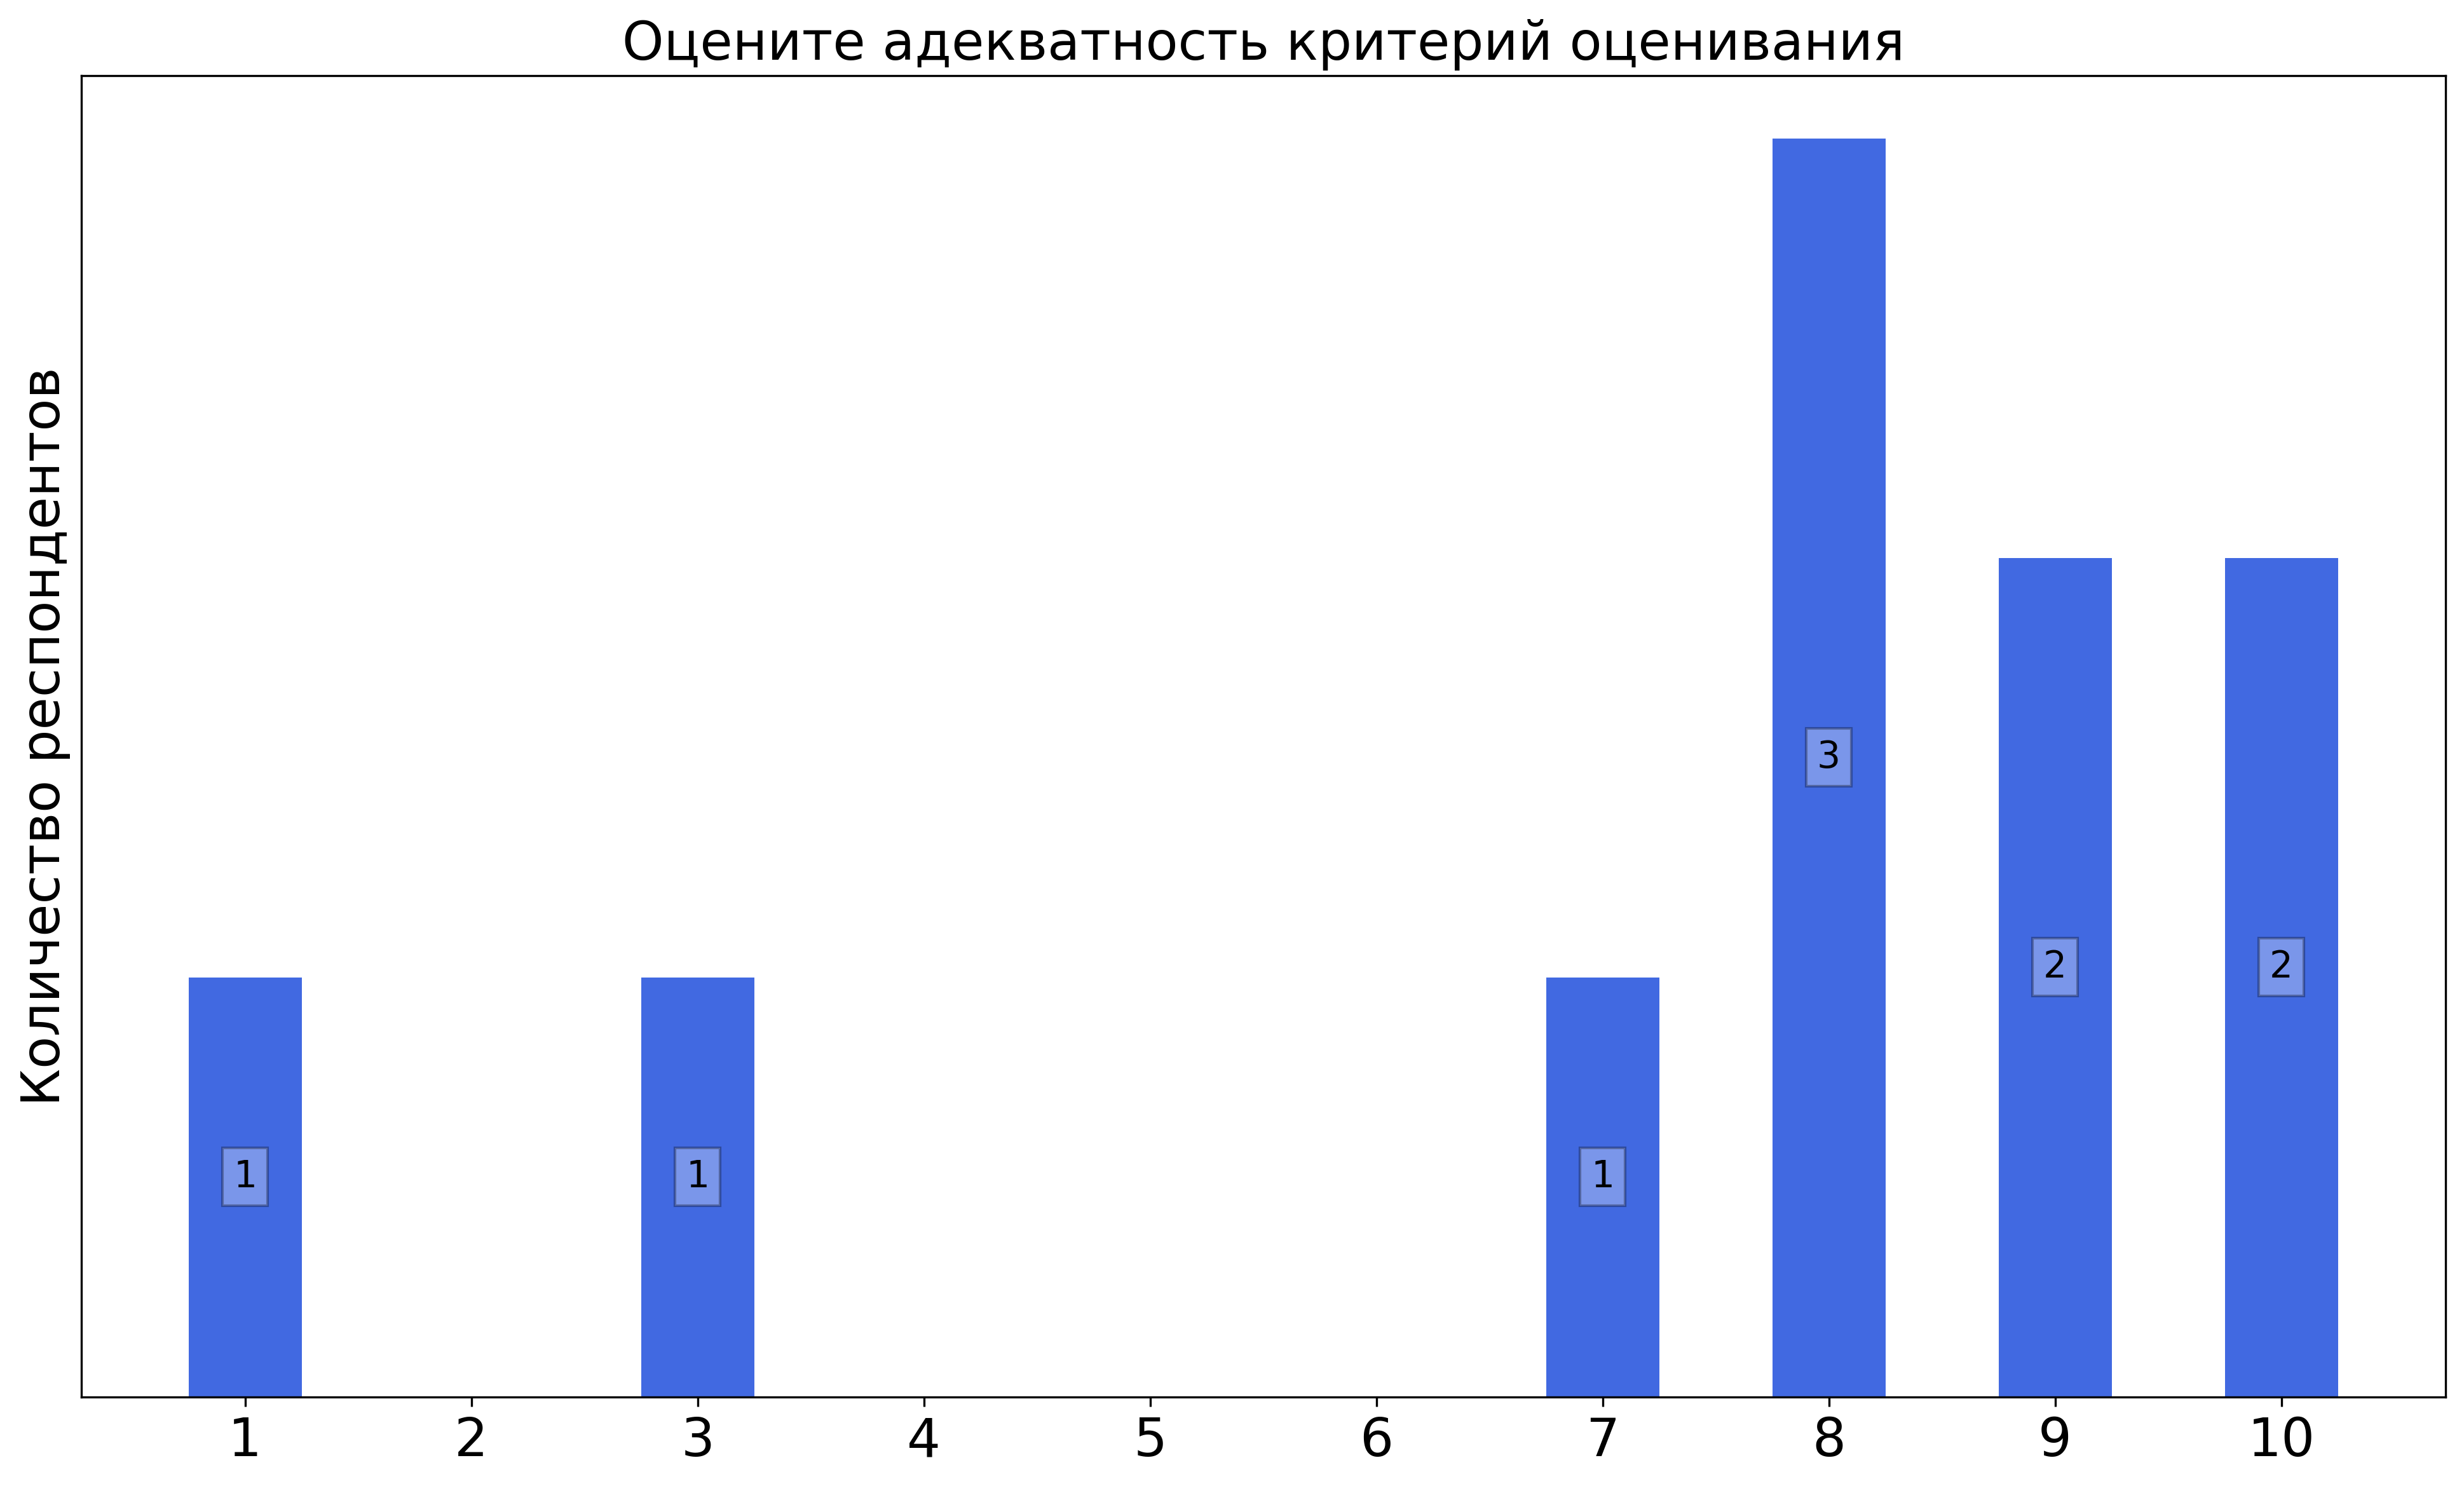
\includegraphics[width=\textwidth]{images/2 course/Компьютерные технологии/seminarists-marks-Кулиев Р.С.-3.png}
            \end{subfigure}	
            \caption{Оценки респондентов о качестве преподавания семинаров}
        \end{figure}

        \textbf{Комментарии студентов о семинаристе\protect\footnote{сохранены оригинальные орфография и пунктуация}}
            \begin{commentbox} 
                Семинары проходили в очень приятной атмосфере  
            \end{commentbox} 
        
            \begin{commentbox} 
                Кулиев - просто ужасный семинарист. Постоянно опаздывает или даже НЕ ПРИХОДИТ на свои пары. Дает задания, но постоянно откладывает их сдачу, а потом жалуется, что никто ничего не успел сдать к концу семестра. Требования есть, а возможность им соответствовать - нет. К семинарам совершенно не готов. Занятия проходят так: к началу приходит пара человек и ждет у двери пока Кулиев придет сам (обычно это спустя 15-20 минут). Кулиев приходит и сразу же жалуется что никого нет. Со временем группа подтягивается, приходит и просто молча и в тишине сидит и занимается своими делами. В это время Кулиев либо сидит своими делами занимается, либо спит, либо ушел на 30+ минут. Если спросить можно ли сдать задание, он скажет "нет, давайте на следующей паре". В итоге, все сдачи проходят на второй половине второй пары. Полторы пары перед этим мы все просто молча сидим. В конце семестра оценки выставляются абсолютно рандомно и в промежутке от хор 5 до отл 8. Подавляющее большинство группы доходит только до половины программы семестра из-за таких сдач. 
            \end{commentbox} 
        
            \begin{commentbox} 
                На семинарах ничего не происходило, преподаватель часто уходил на 40 и более минут, практически ничего не рассказывая по теме 
            \end{commentbox} 
        
            \begin{commentbox} 
                Не приходит на семинары. 
            \end{commentbox}


    
    \subsubsection{Отзыв студентов о семинарах. Семинарист: Пудгородский Ю.А.}
        \begin{figure}[H]
            \centering
            \begin{subfigure}[b]{0.45\textwidth}
                \centering
                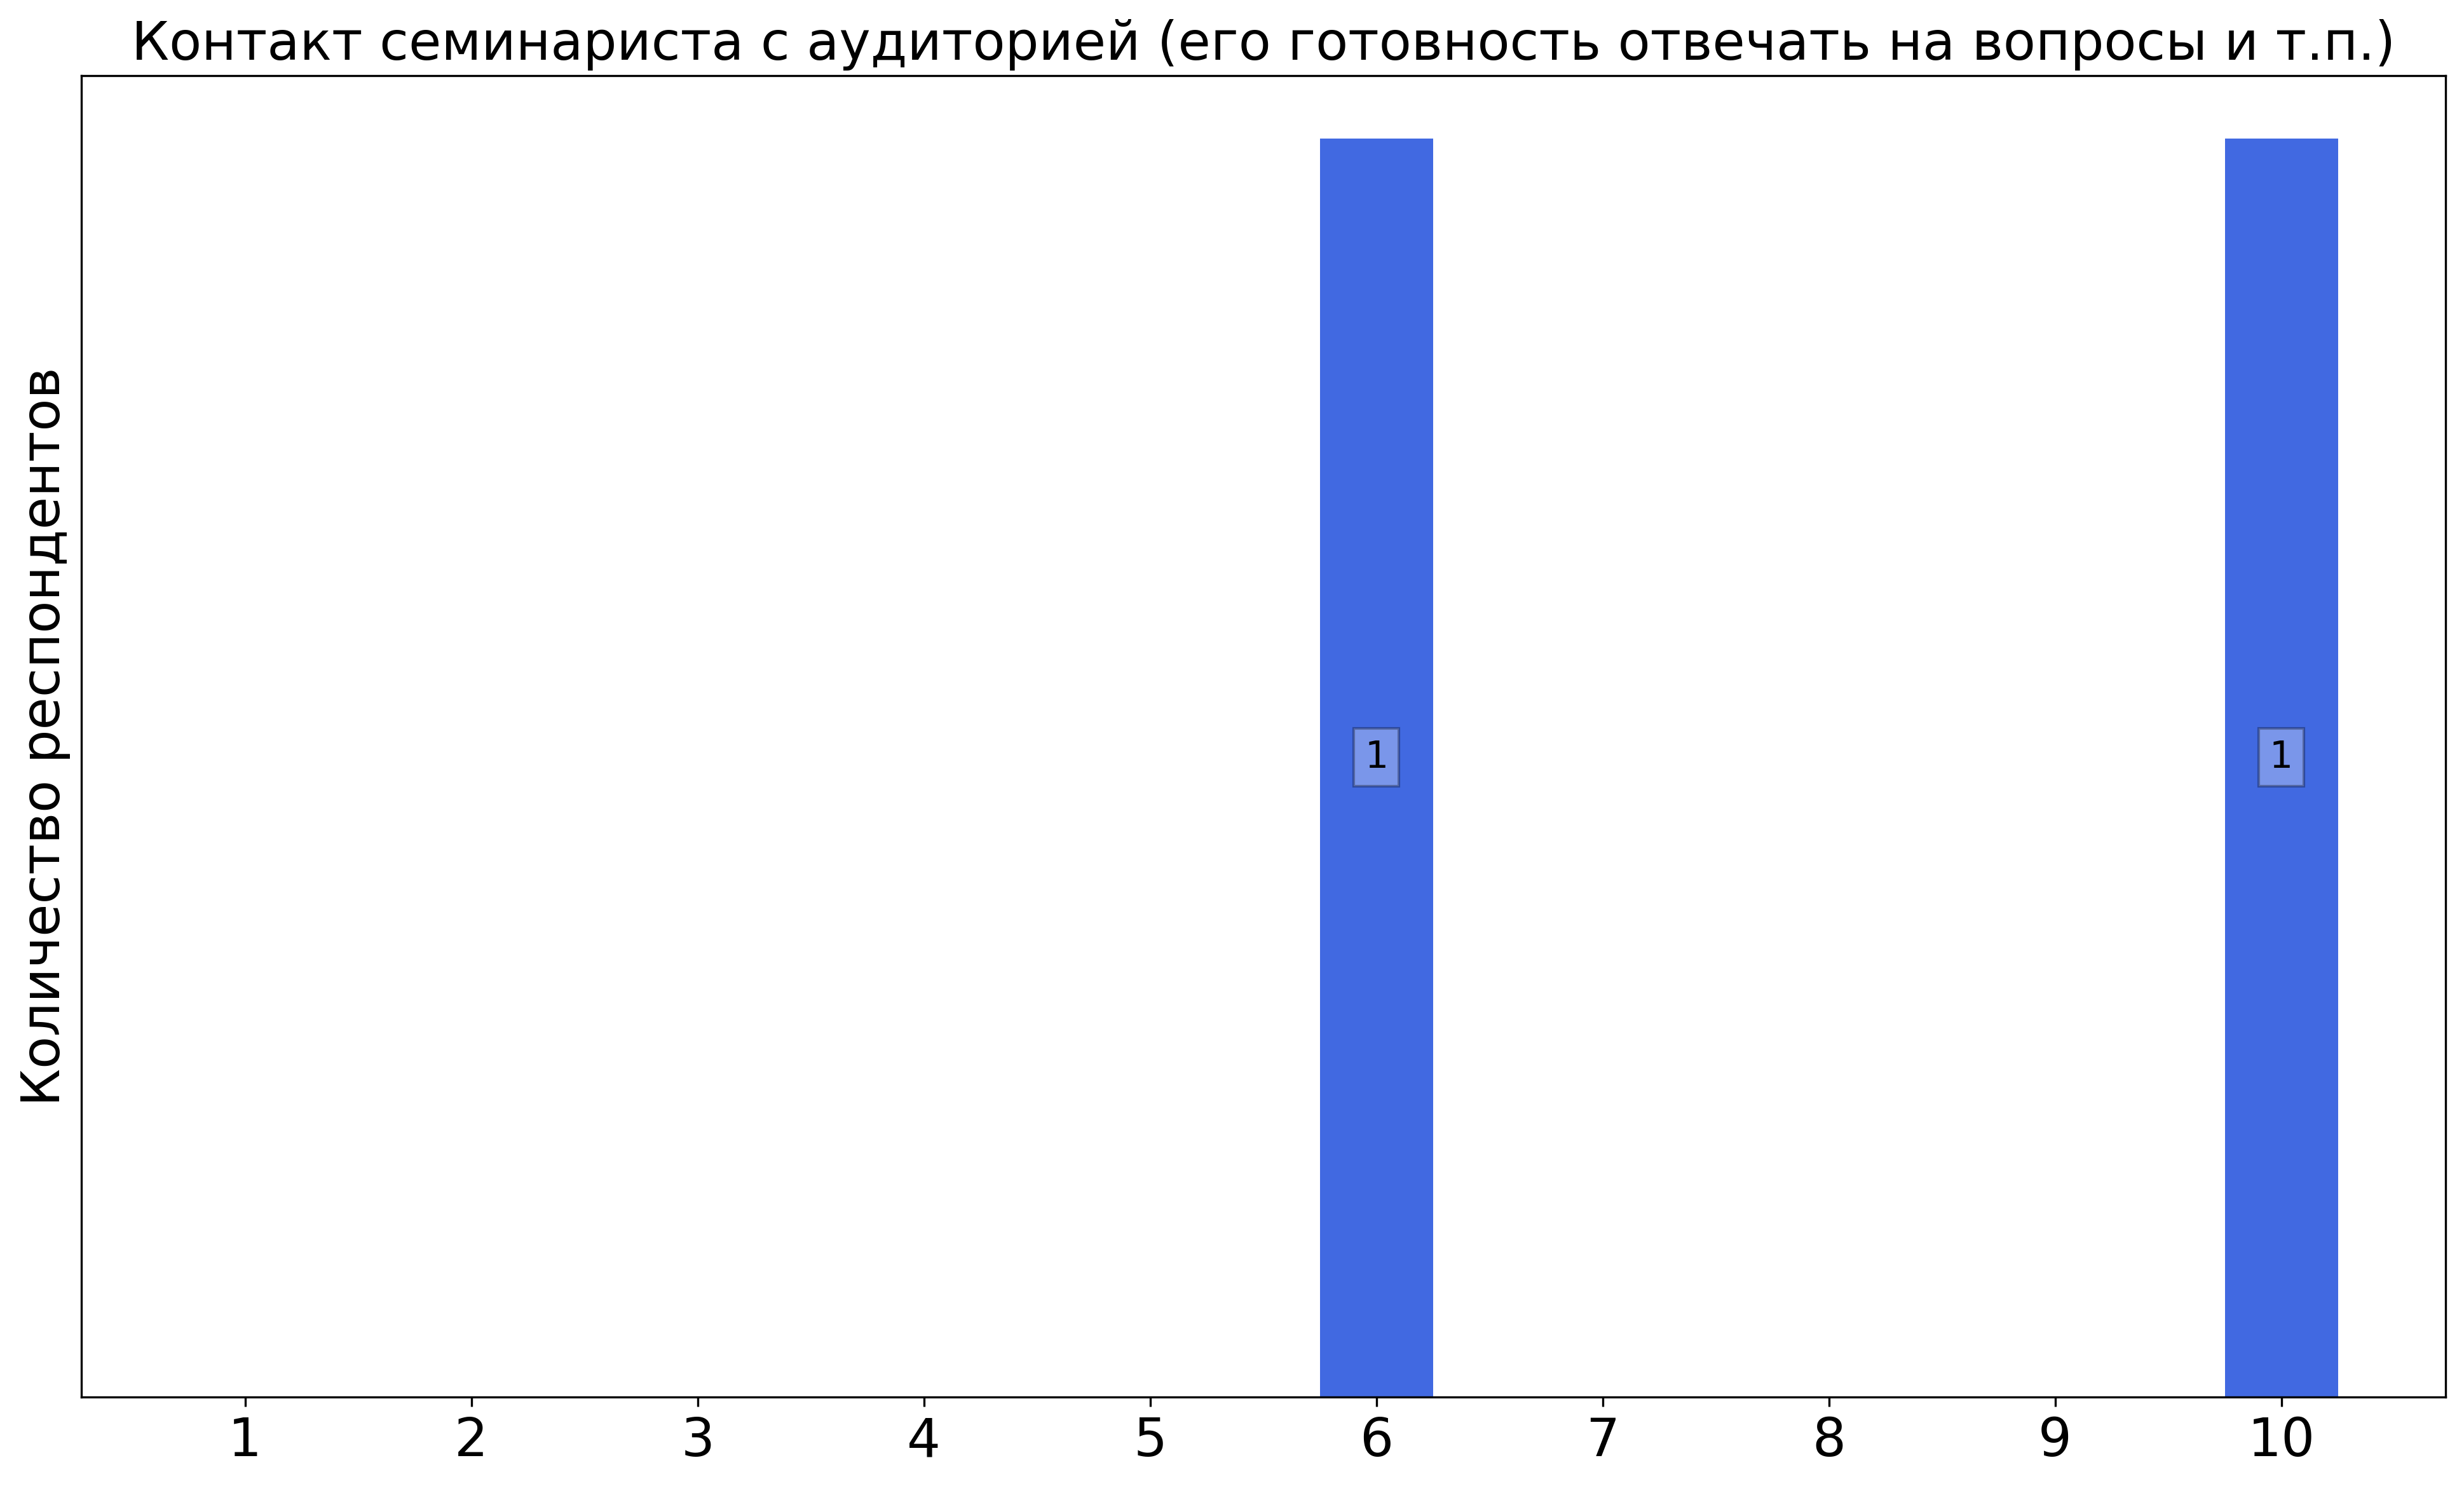
\includegraphics[width=\textwidth]{images/2 course/Компьютерные технологии/seminarists-marks-Пудгородский Ю.А.-0.png}
            \end{subfigure}
            \begin{subfigure}[b]{0.45\textwidth}
                \centering
                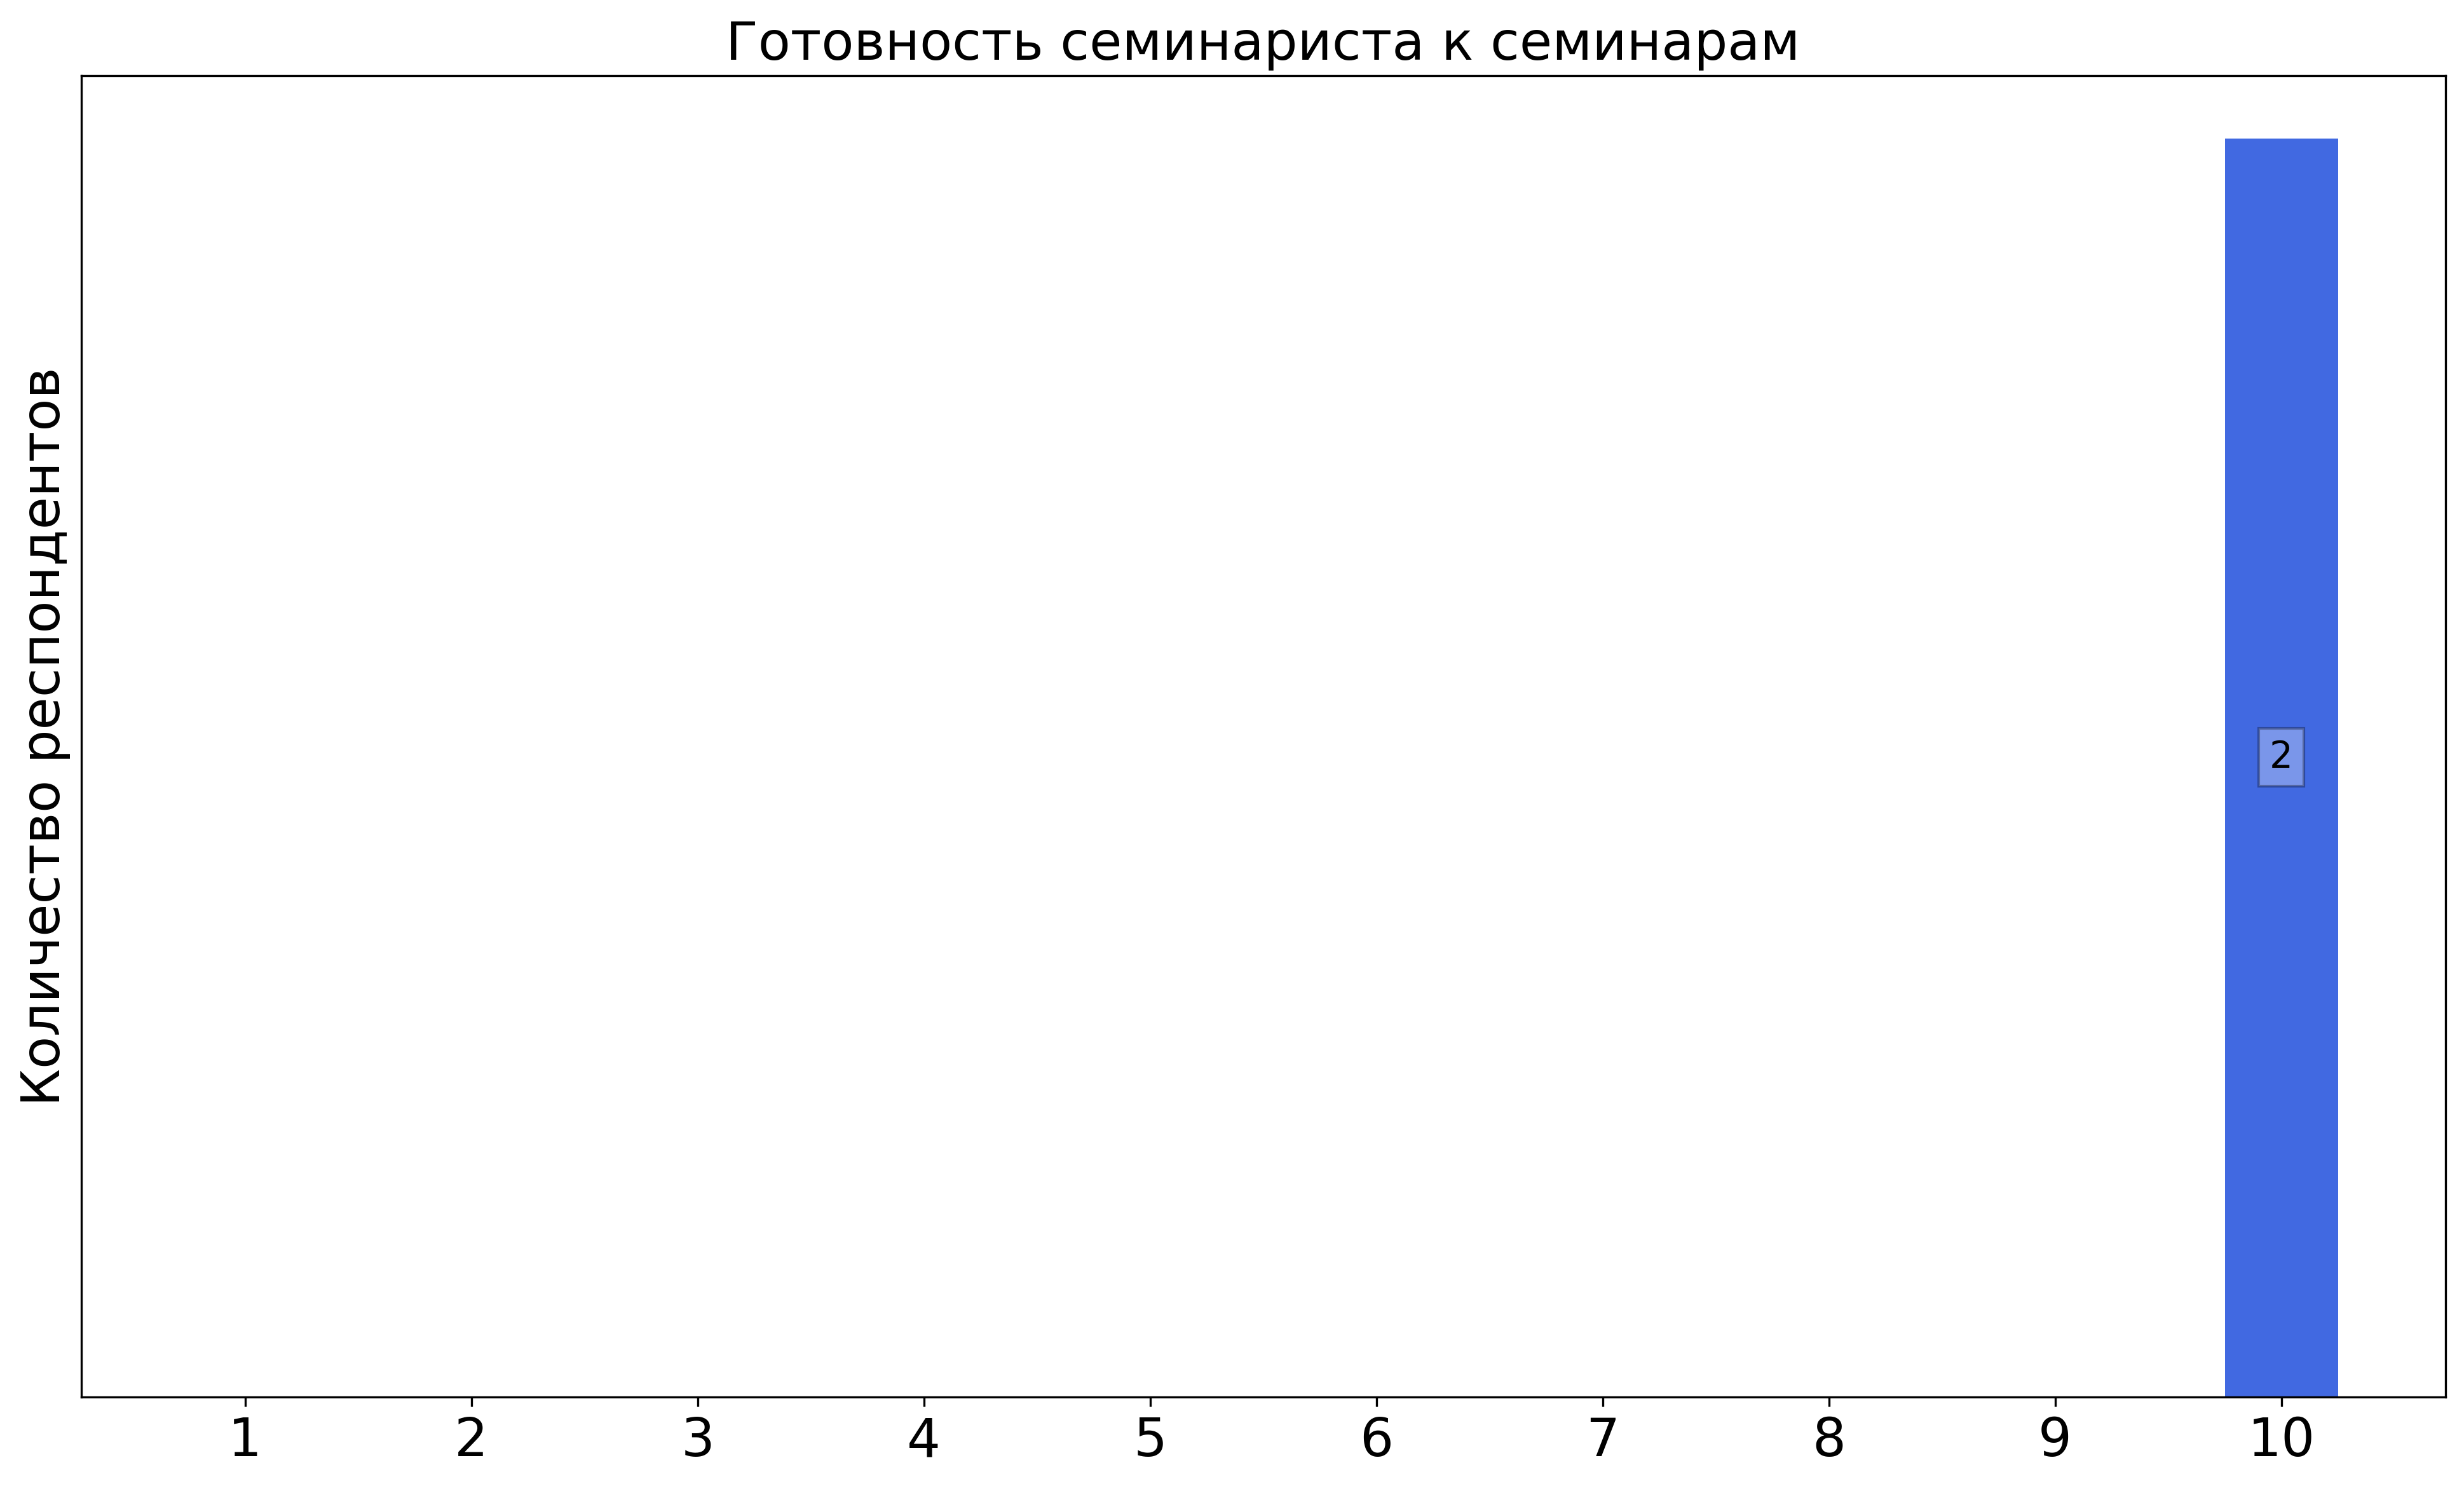
\includegraphics[width=\textwidth]{images/2 course/Компьютерные технологии/seminarists-marks-Пудгородский Ю.А.-1.png}
            \end{subfigure}
            \begin{subfigure}[b]{0.45\textwidth}
                \centering
                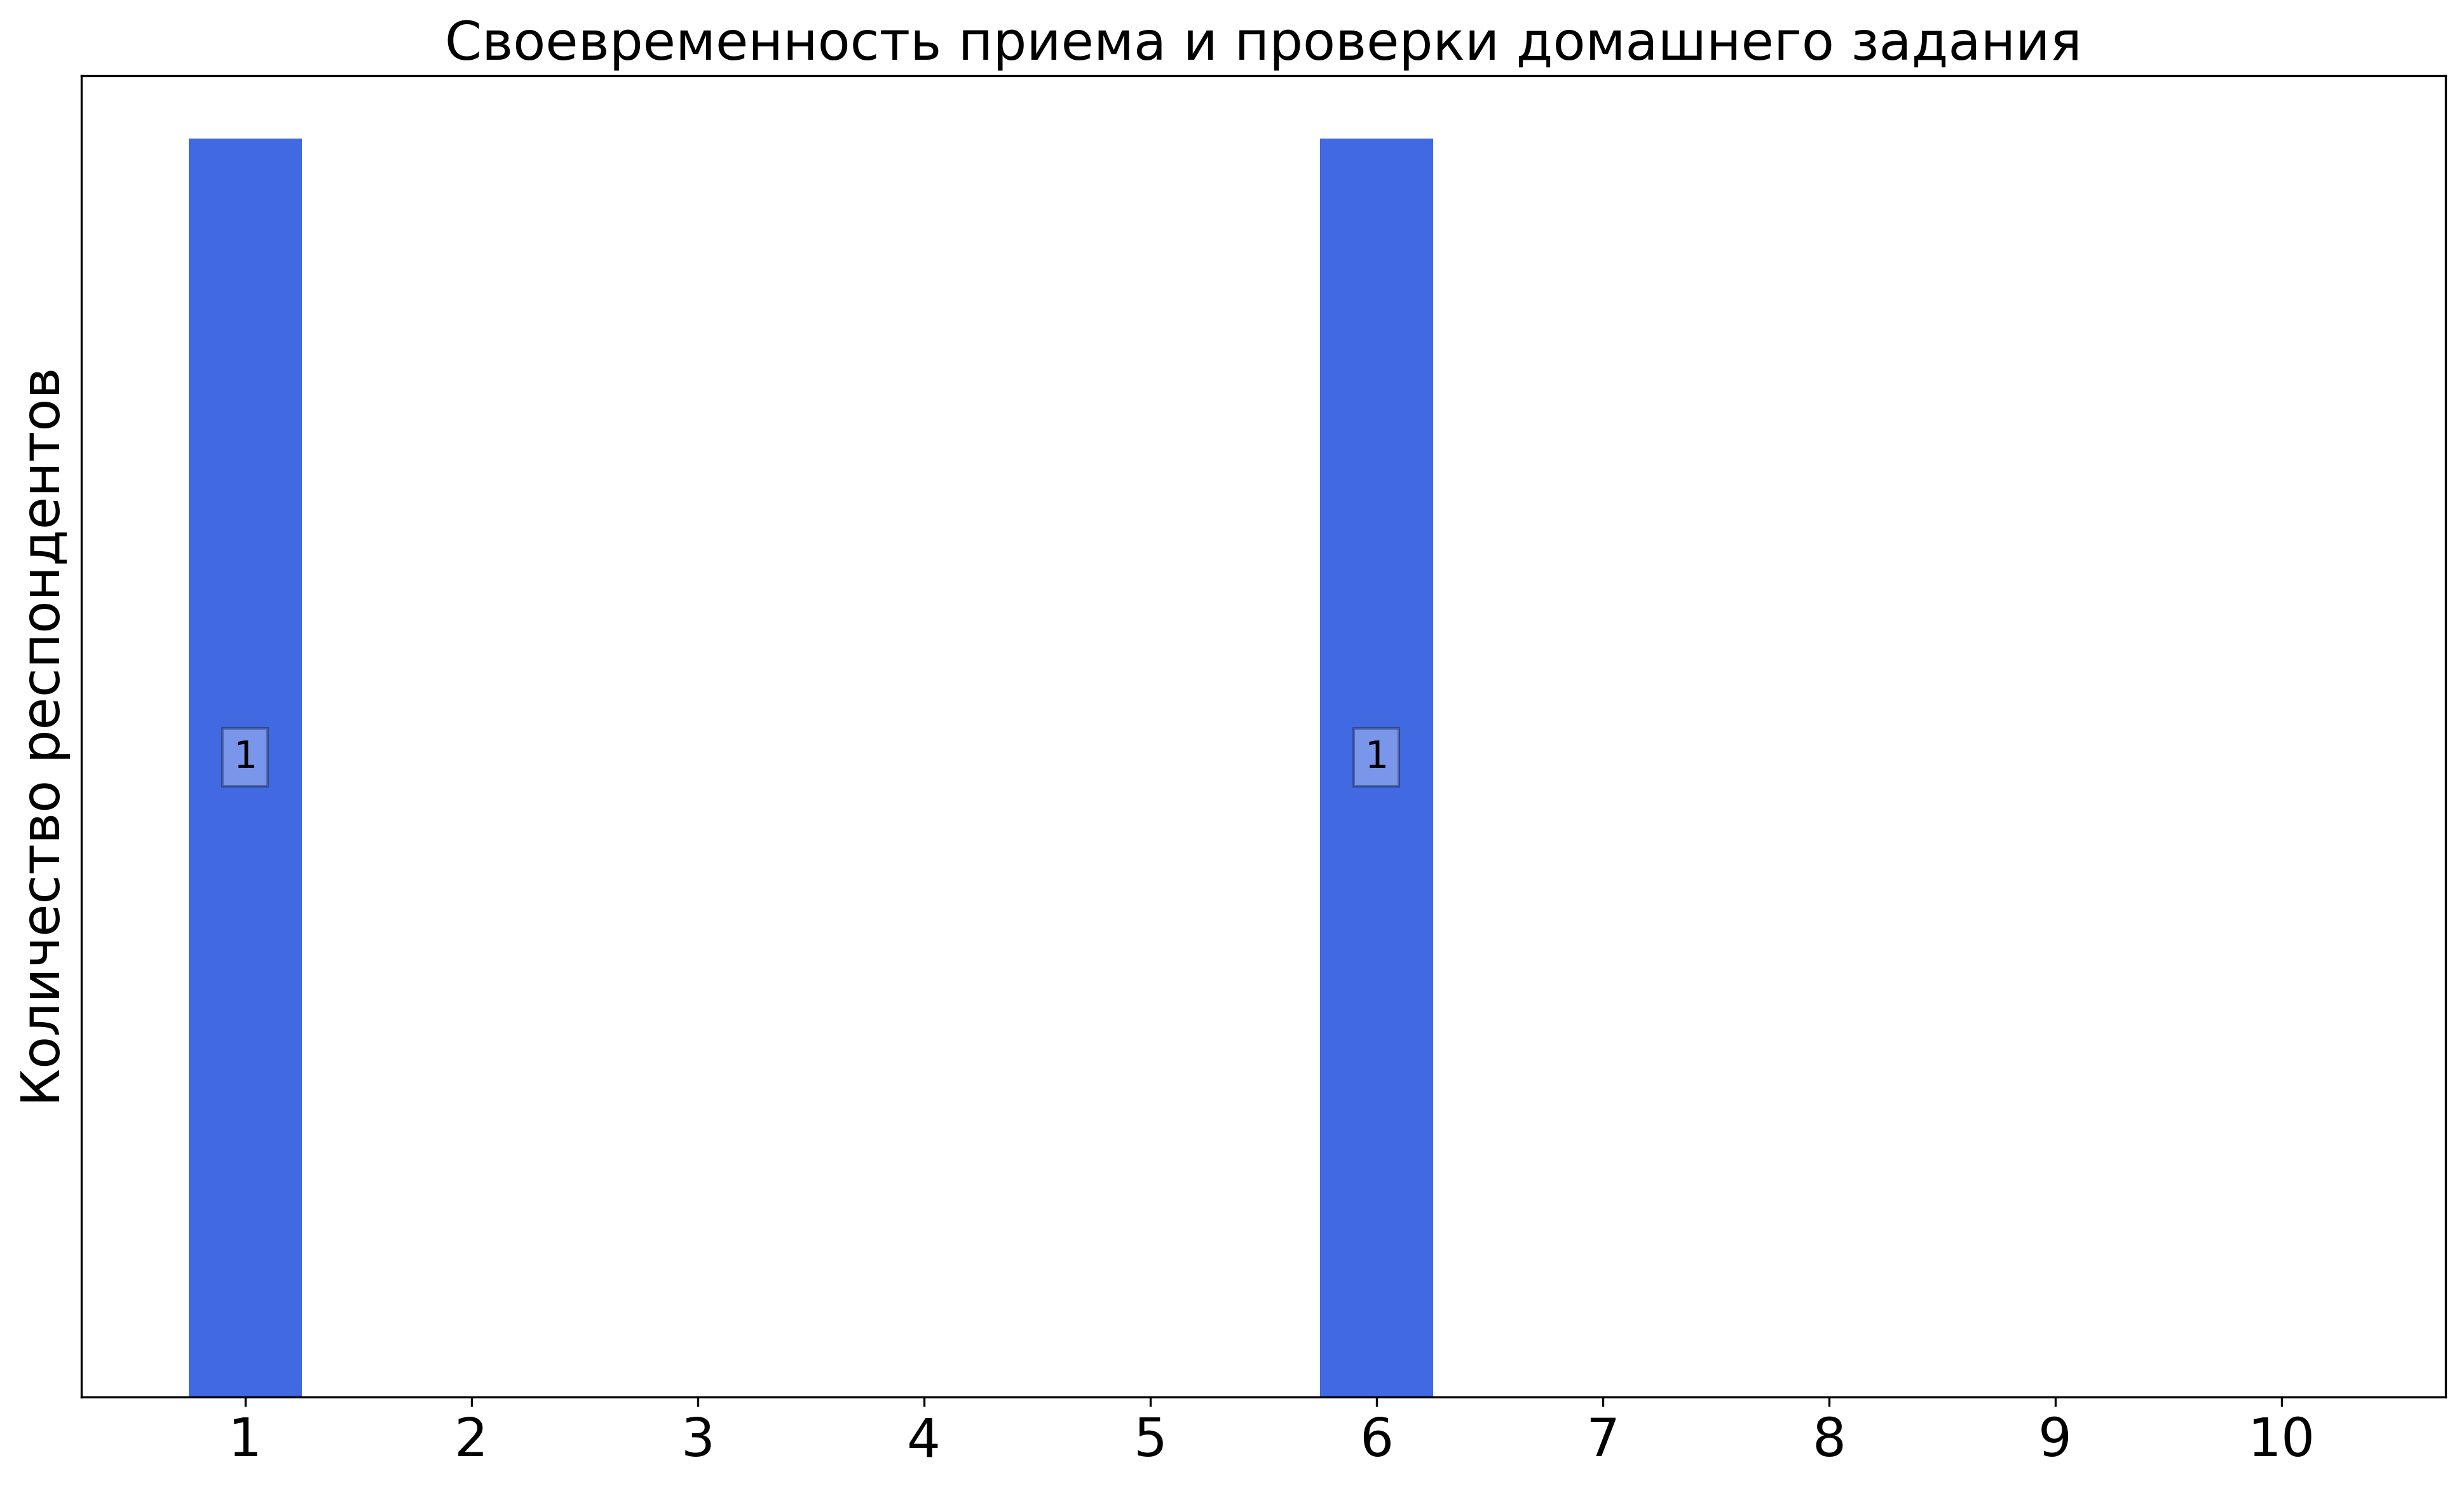
\includegraphics[width=\textwidth]{images/2 course/Компьютерные технологии/seminarists-marks-Пудгородский Ю.А.-2.png}
            \end{subfigure}
            \begin{subfigure}[b]{0.45\textwidth}
                \centering
                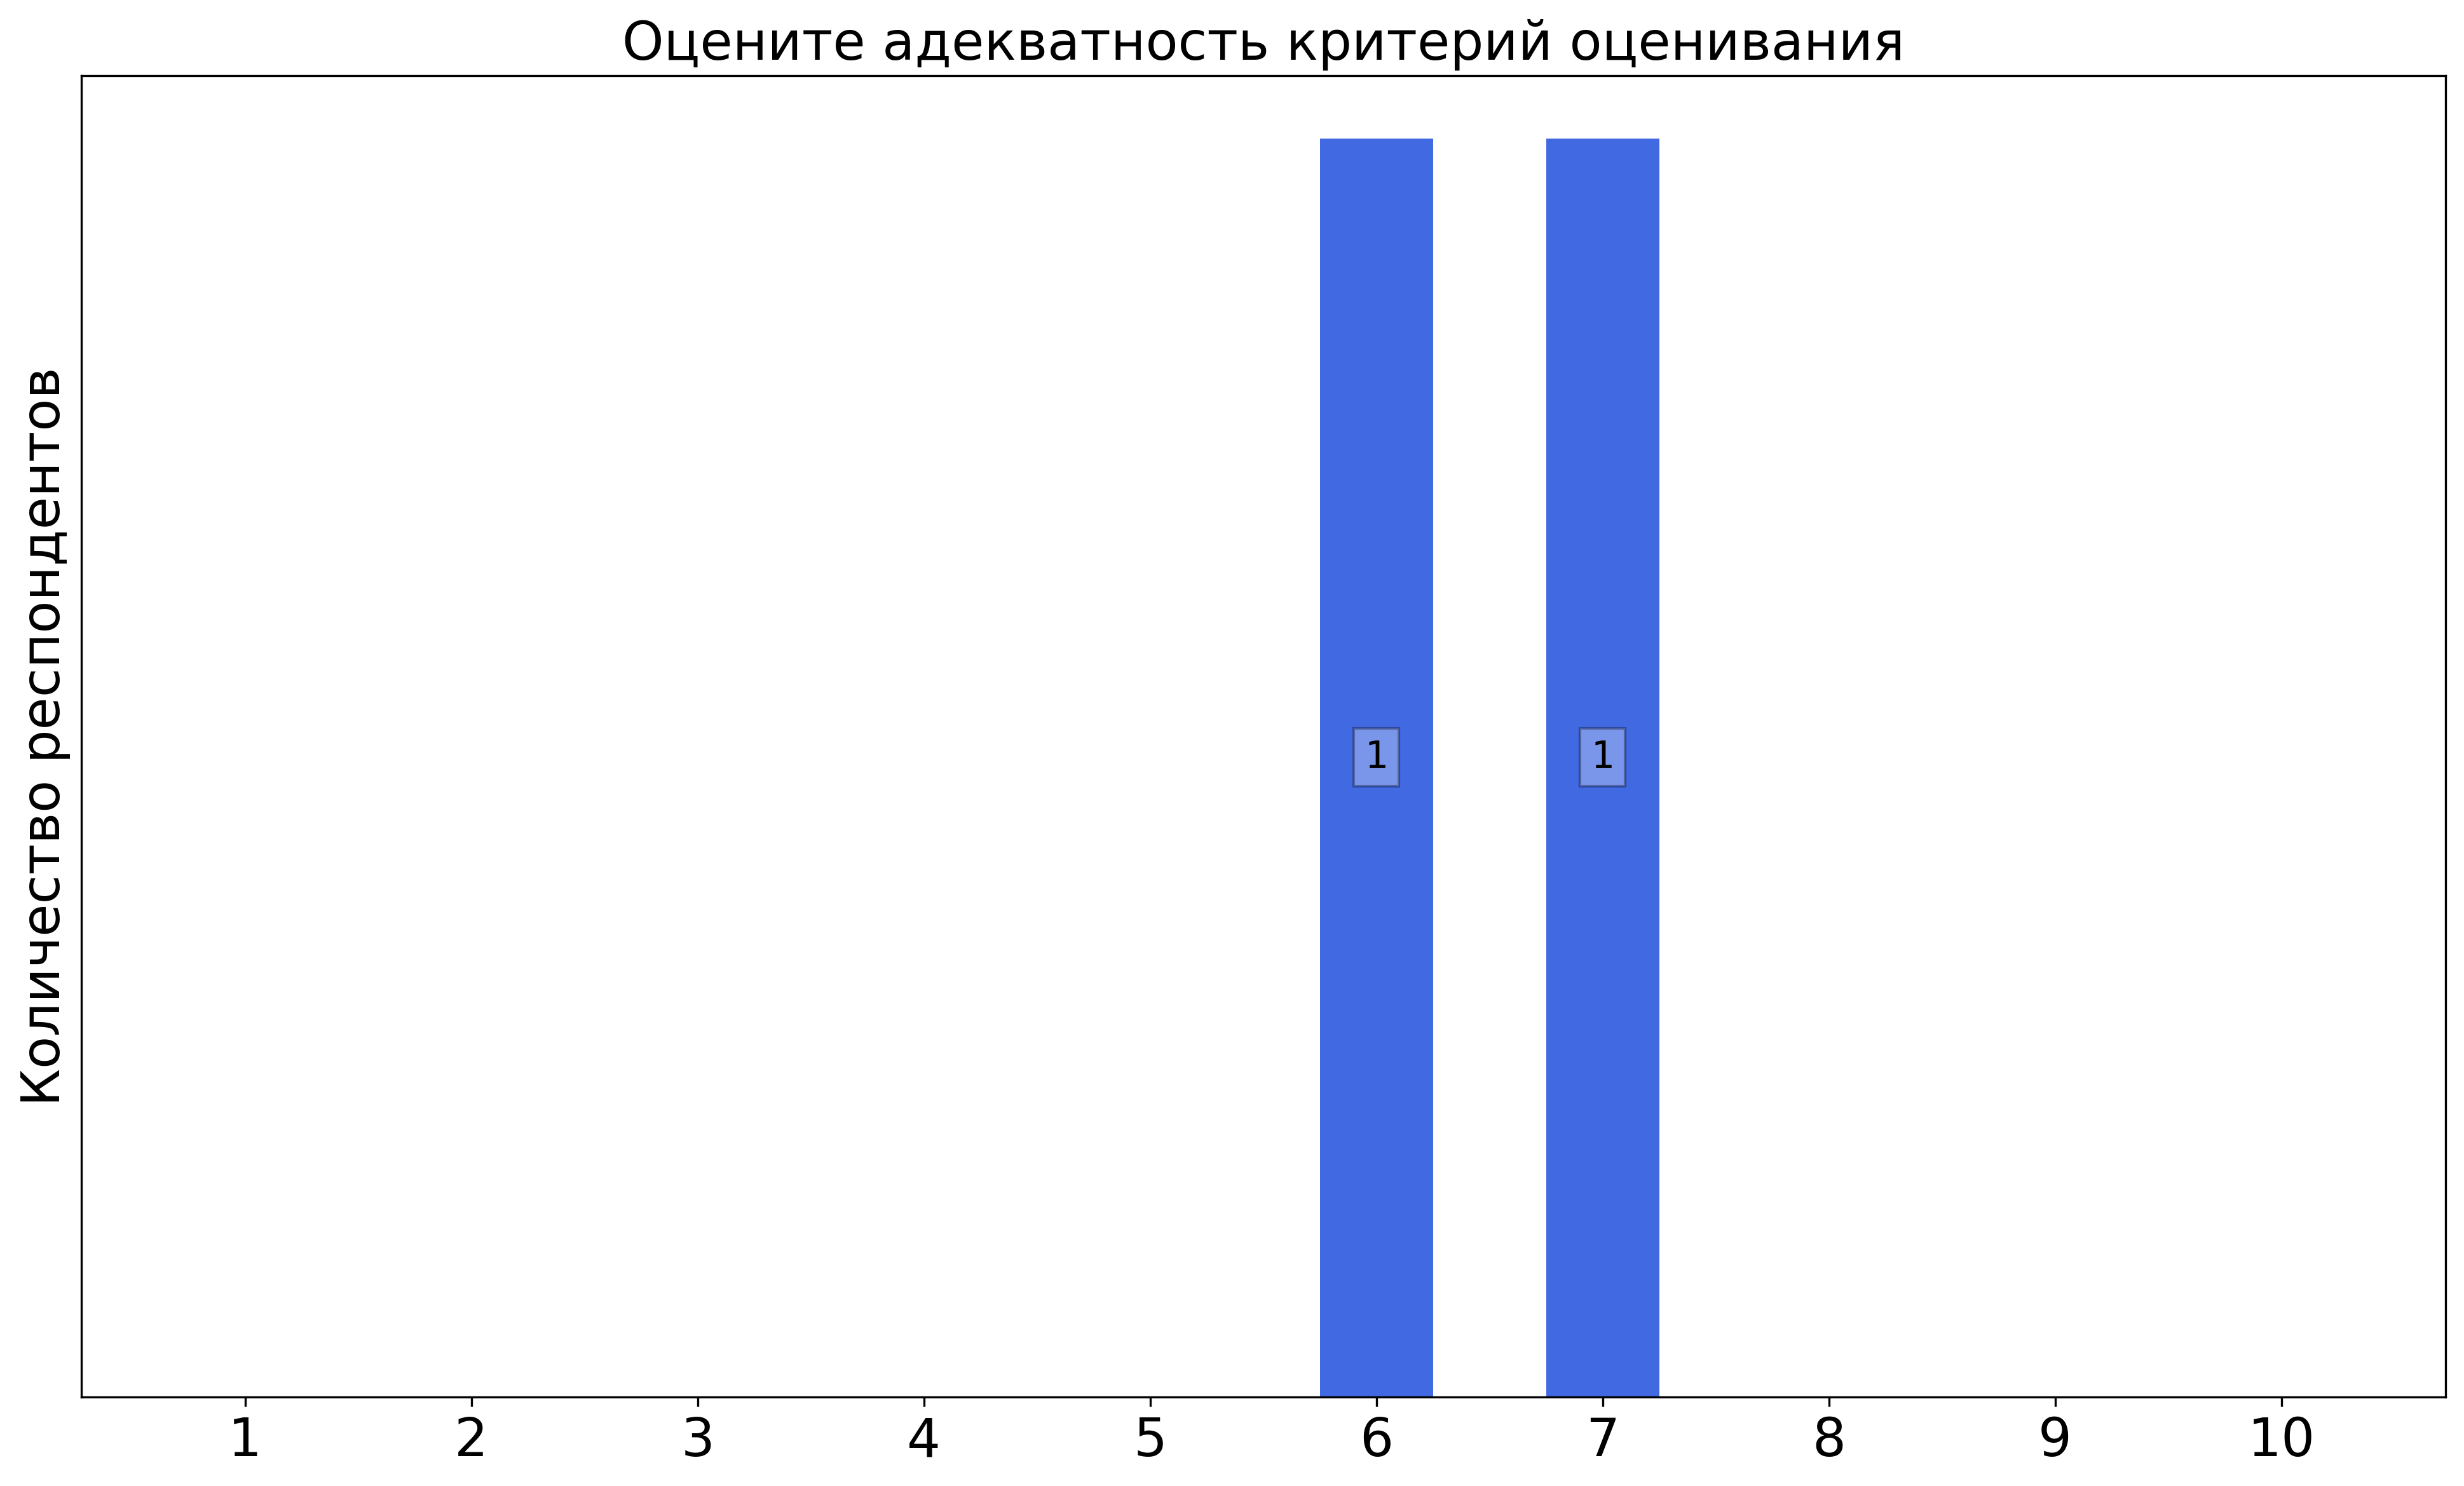
\includegraphics[width=\textwidth]{images/2 course/Компьютерные технологии/seminarists-marks-Пудгородский Ю.А.-3.png}
            \end{subfigure}	
            \caption{Оценки респондентов о качестве преподавания семинаров}
        \end{figure}

        \textbf{Комментарии студентов о семинаристе\protect\footnote{сохранены оригинальные орфография и пунктуация}}
            \begin{commentbox} 
                Всегда опаздывал, и достаточно сложно объяснял 
            \end{commentbox}

    
    \subsubsection{Отзыв студентов о семинарах. Семинарист: Чуканова О.В.}
        \begin{figure}[H]
            \centering
            \begin{subfigure}[b]{0.45\textwidth}
                \centering
                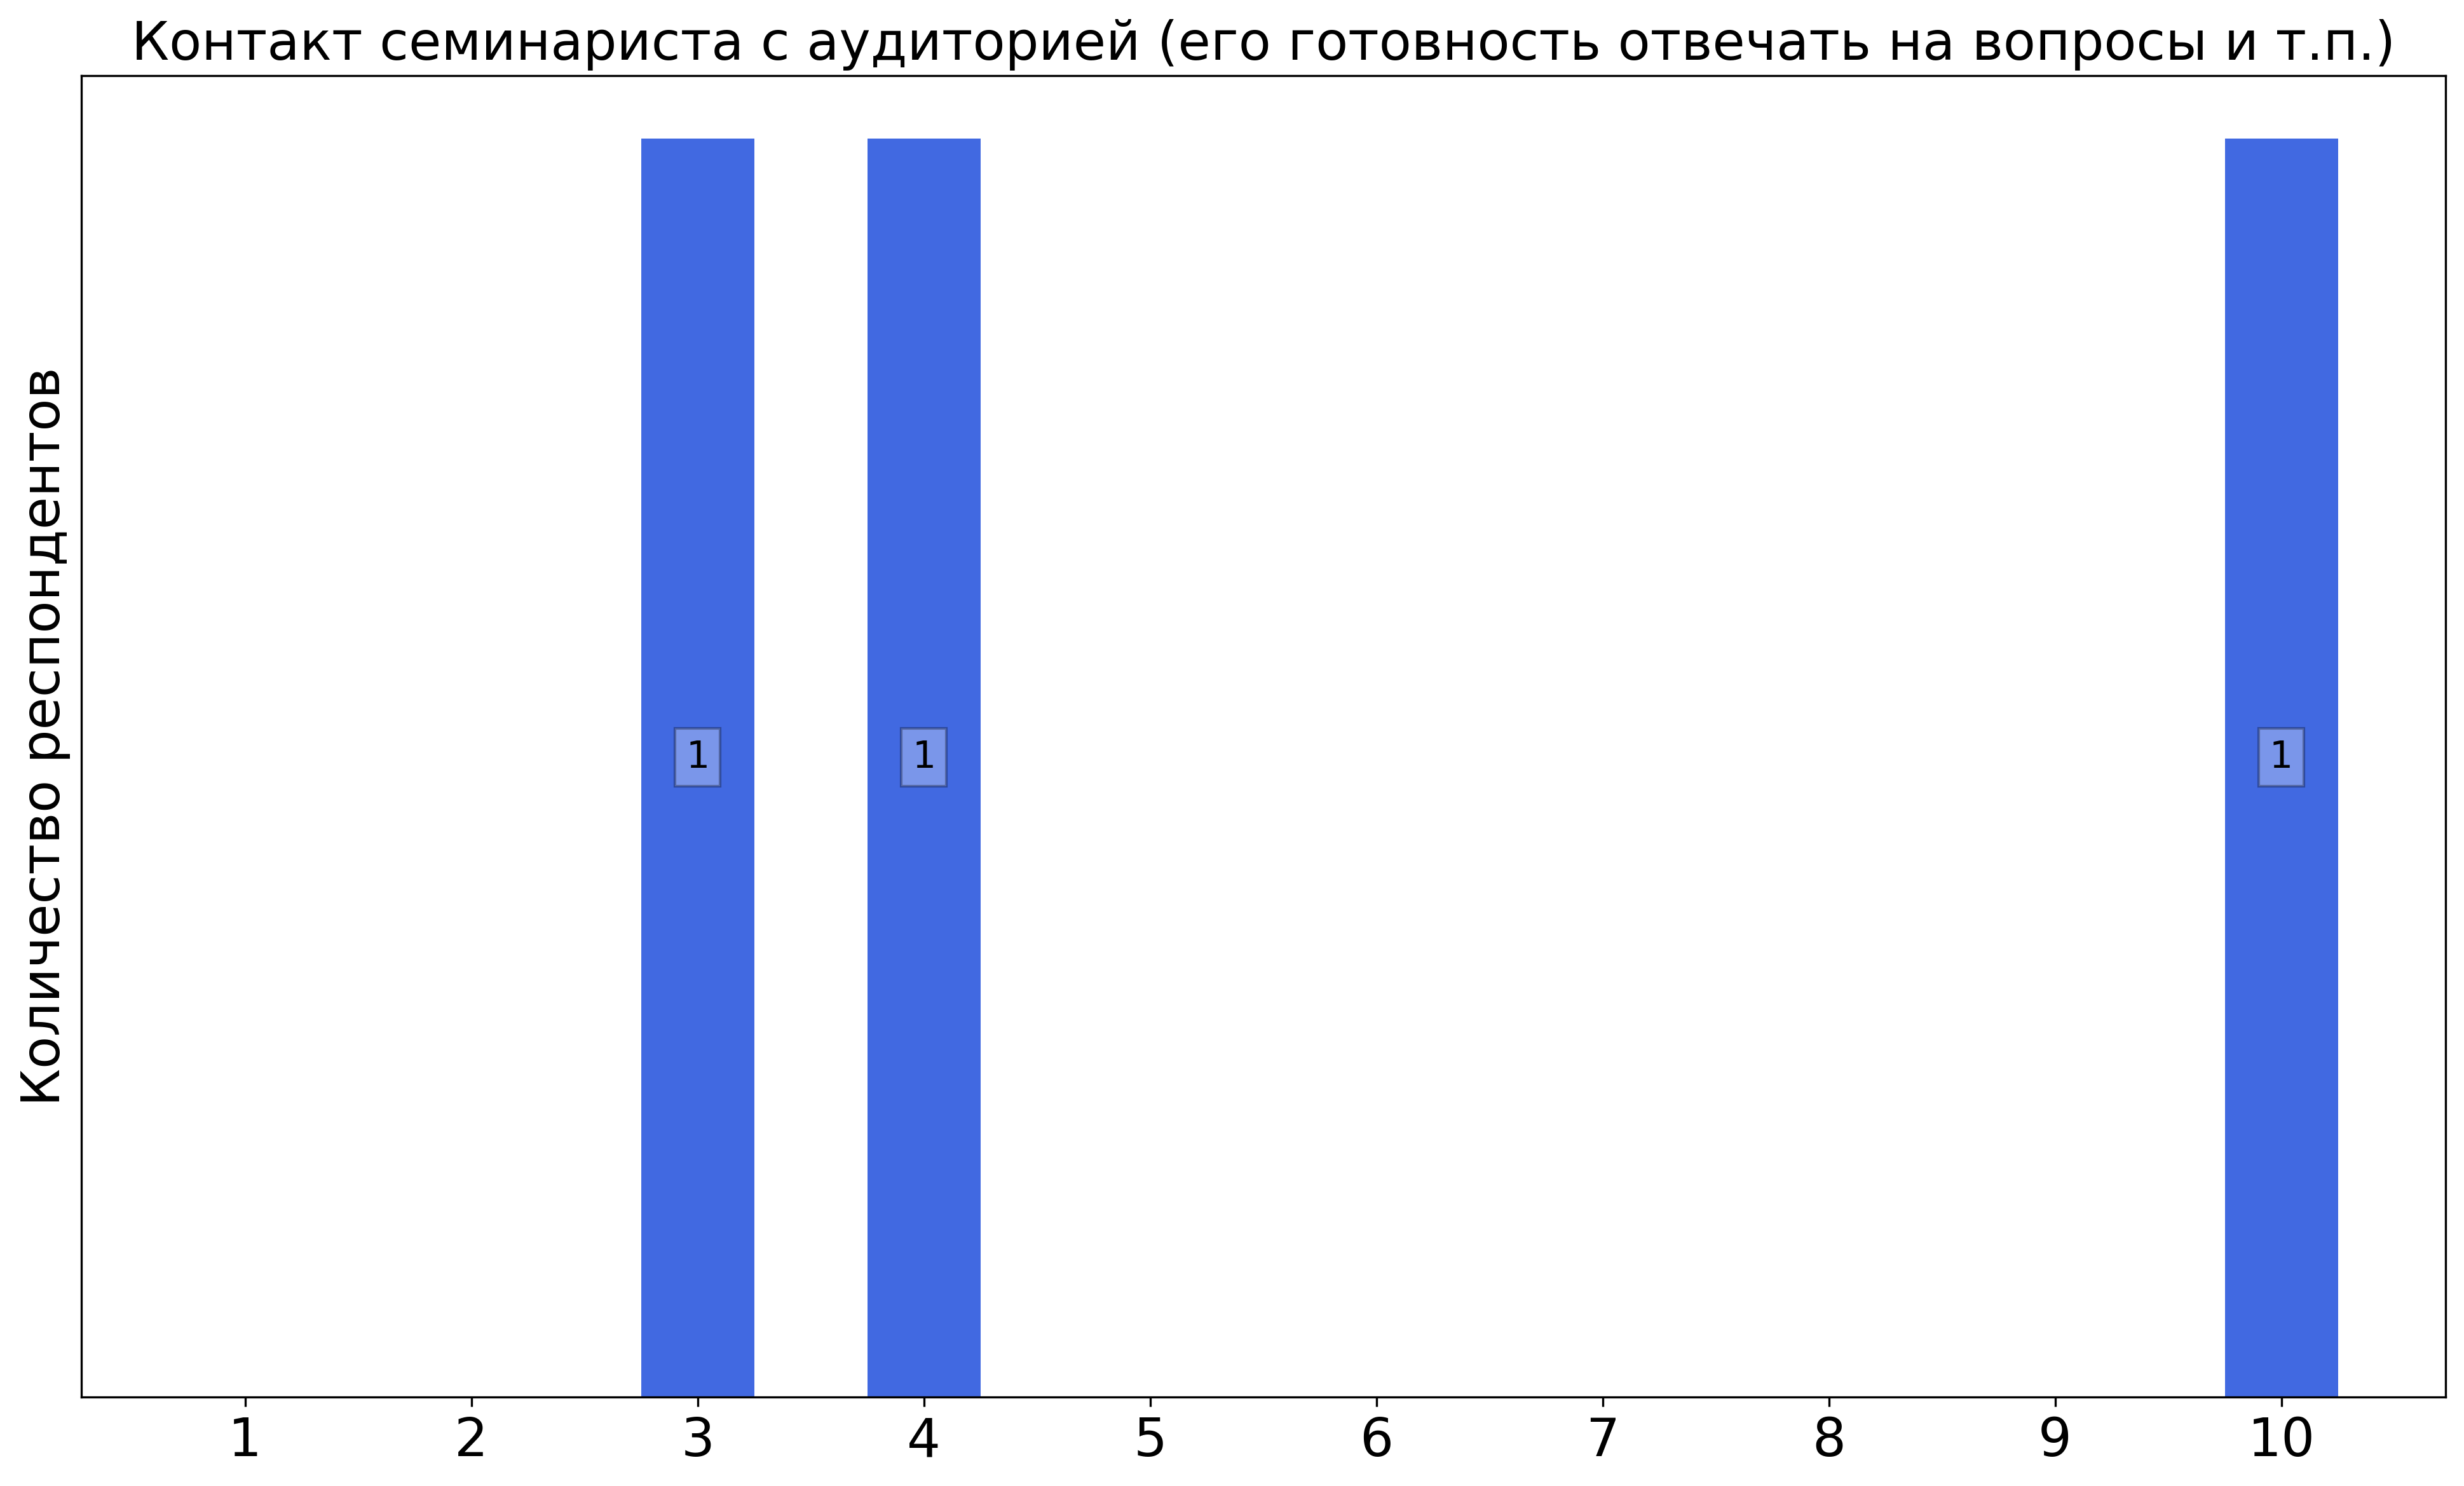
\includegraphics[width=\textwidth]{images/2 course/Компьютерные технологии/seminarists-marks-Чуканова О.В.-0.png}
            \end{subfigure}
            \begin{subfigure}[b]{0.45\textwidth}
                \centering
                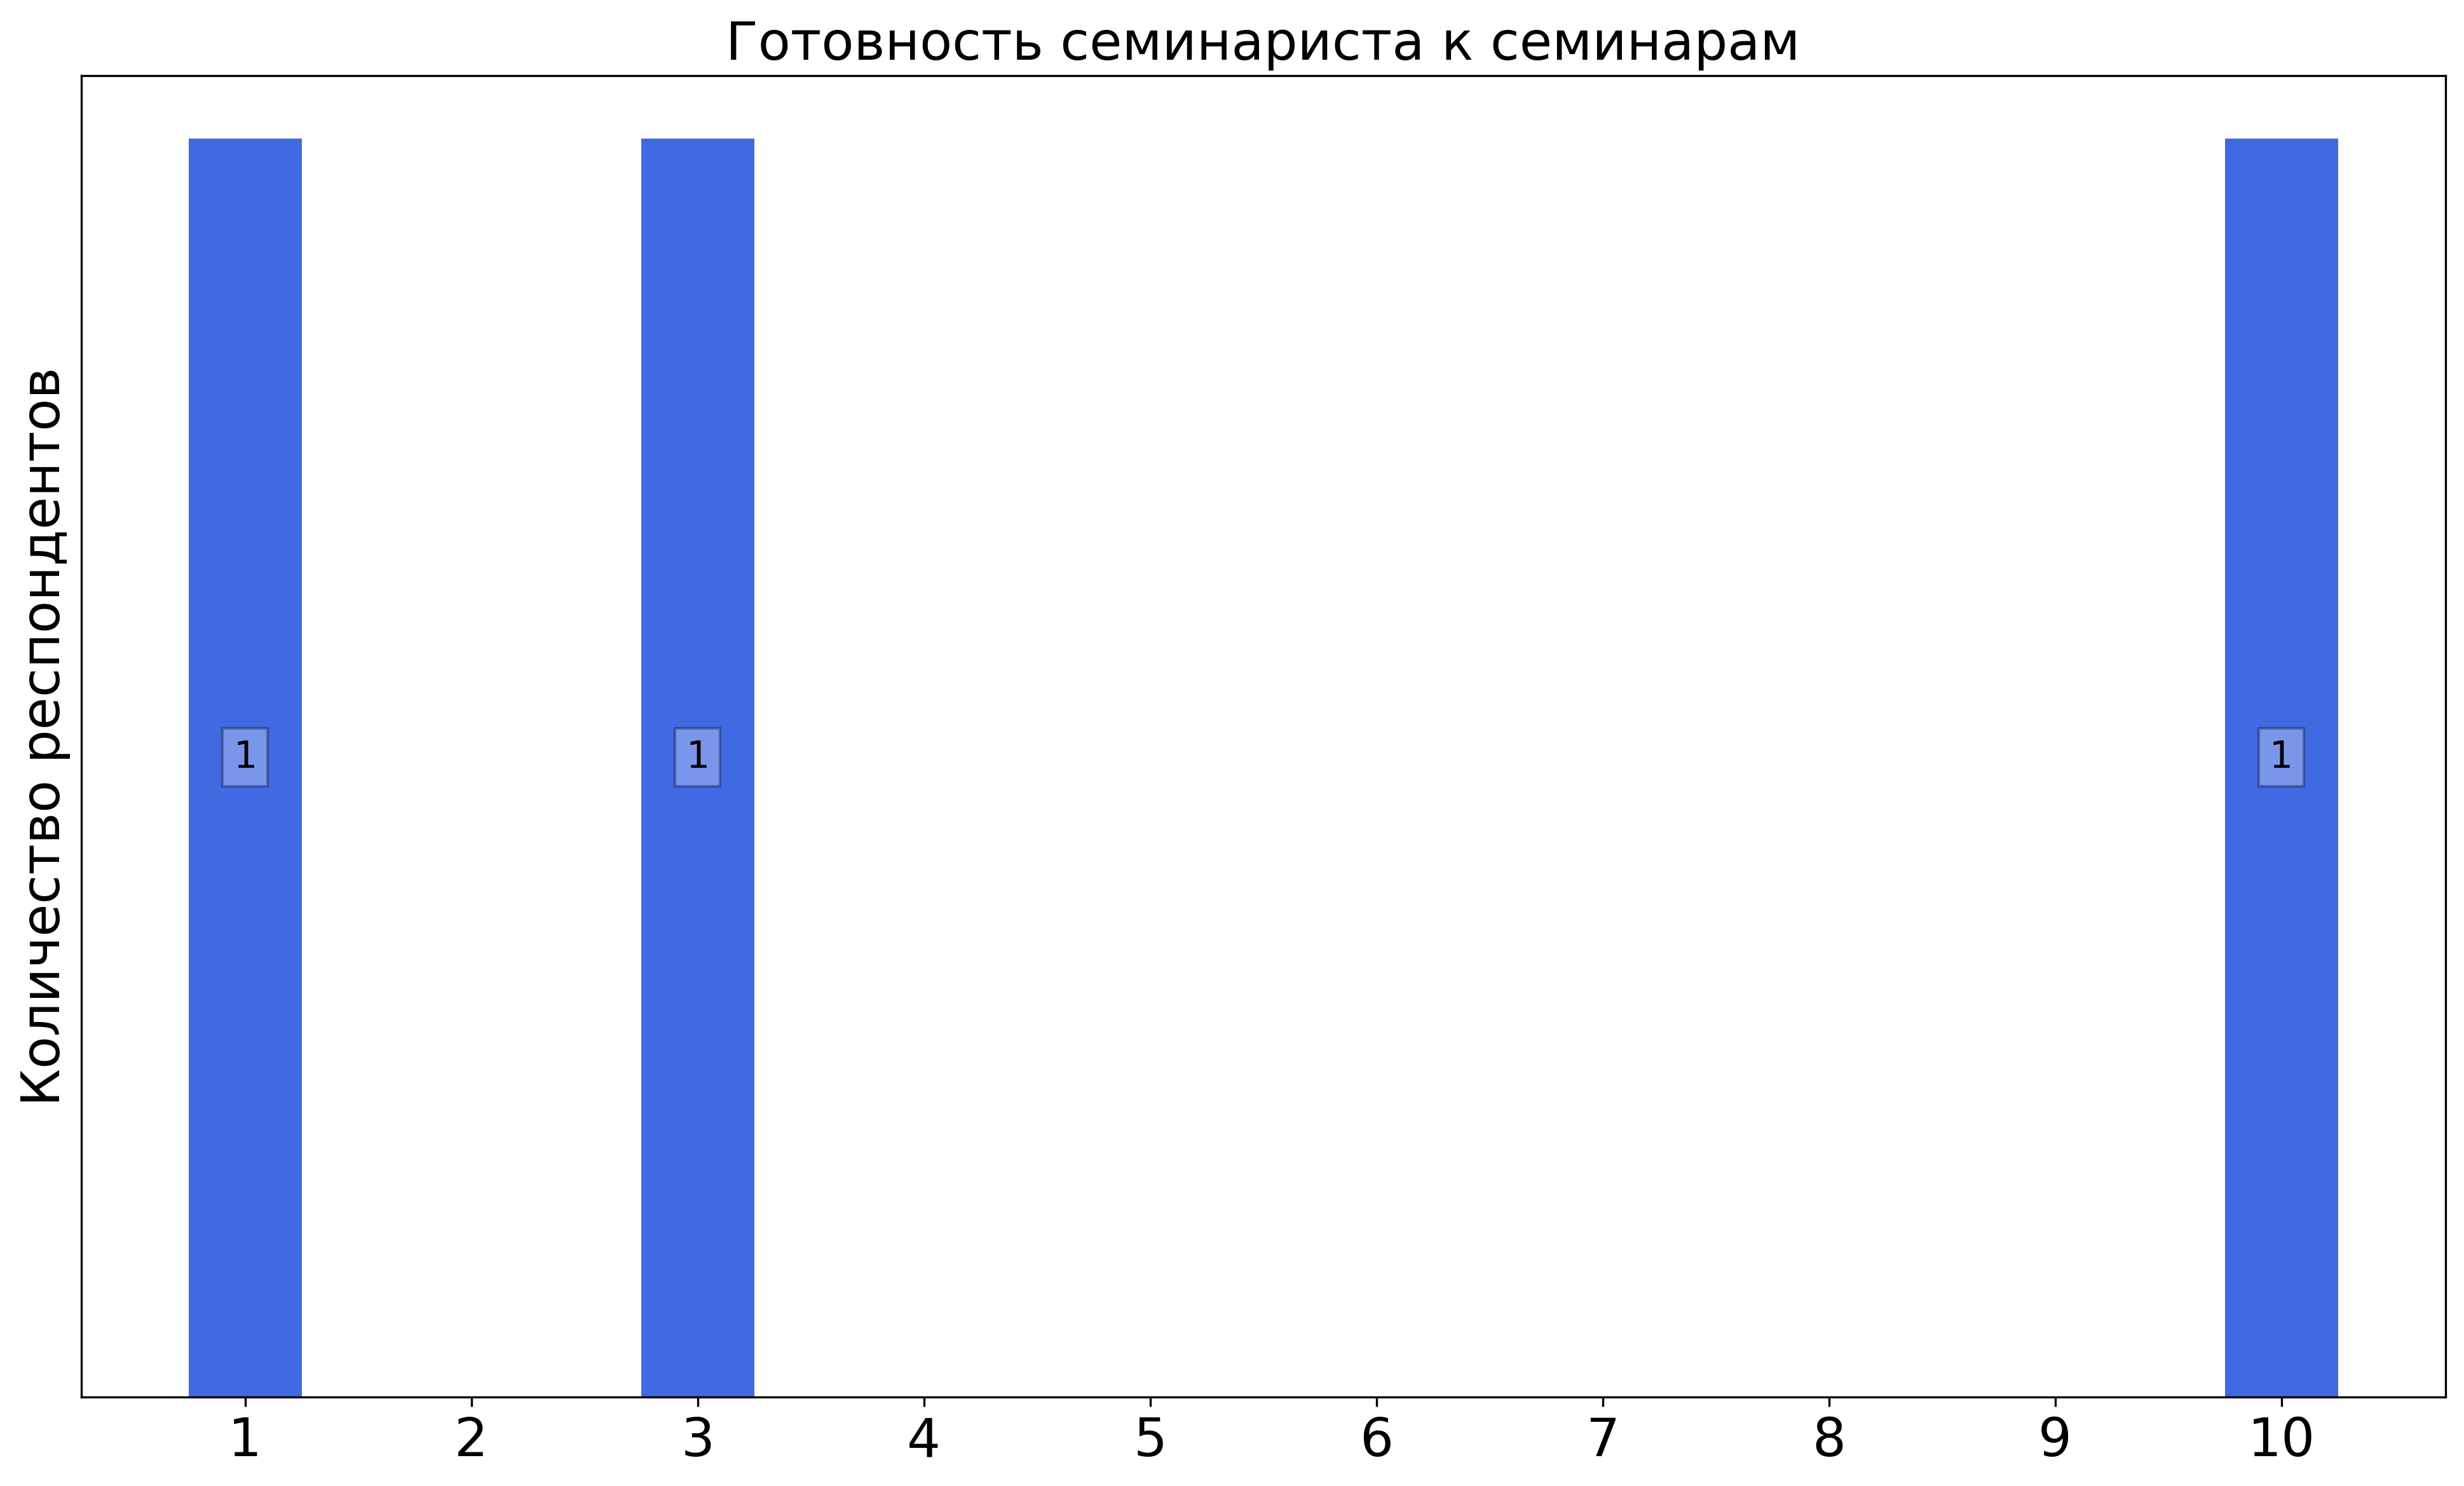
\includegraphics[width=\textwidth]{images/2 course/Компьютерные технологии/seminarists-marks-Чуканова О.В.-1.png}
            \end{subfigure}
            \begin{subfigure}[b]{0.45\textwidth}
                \centering
                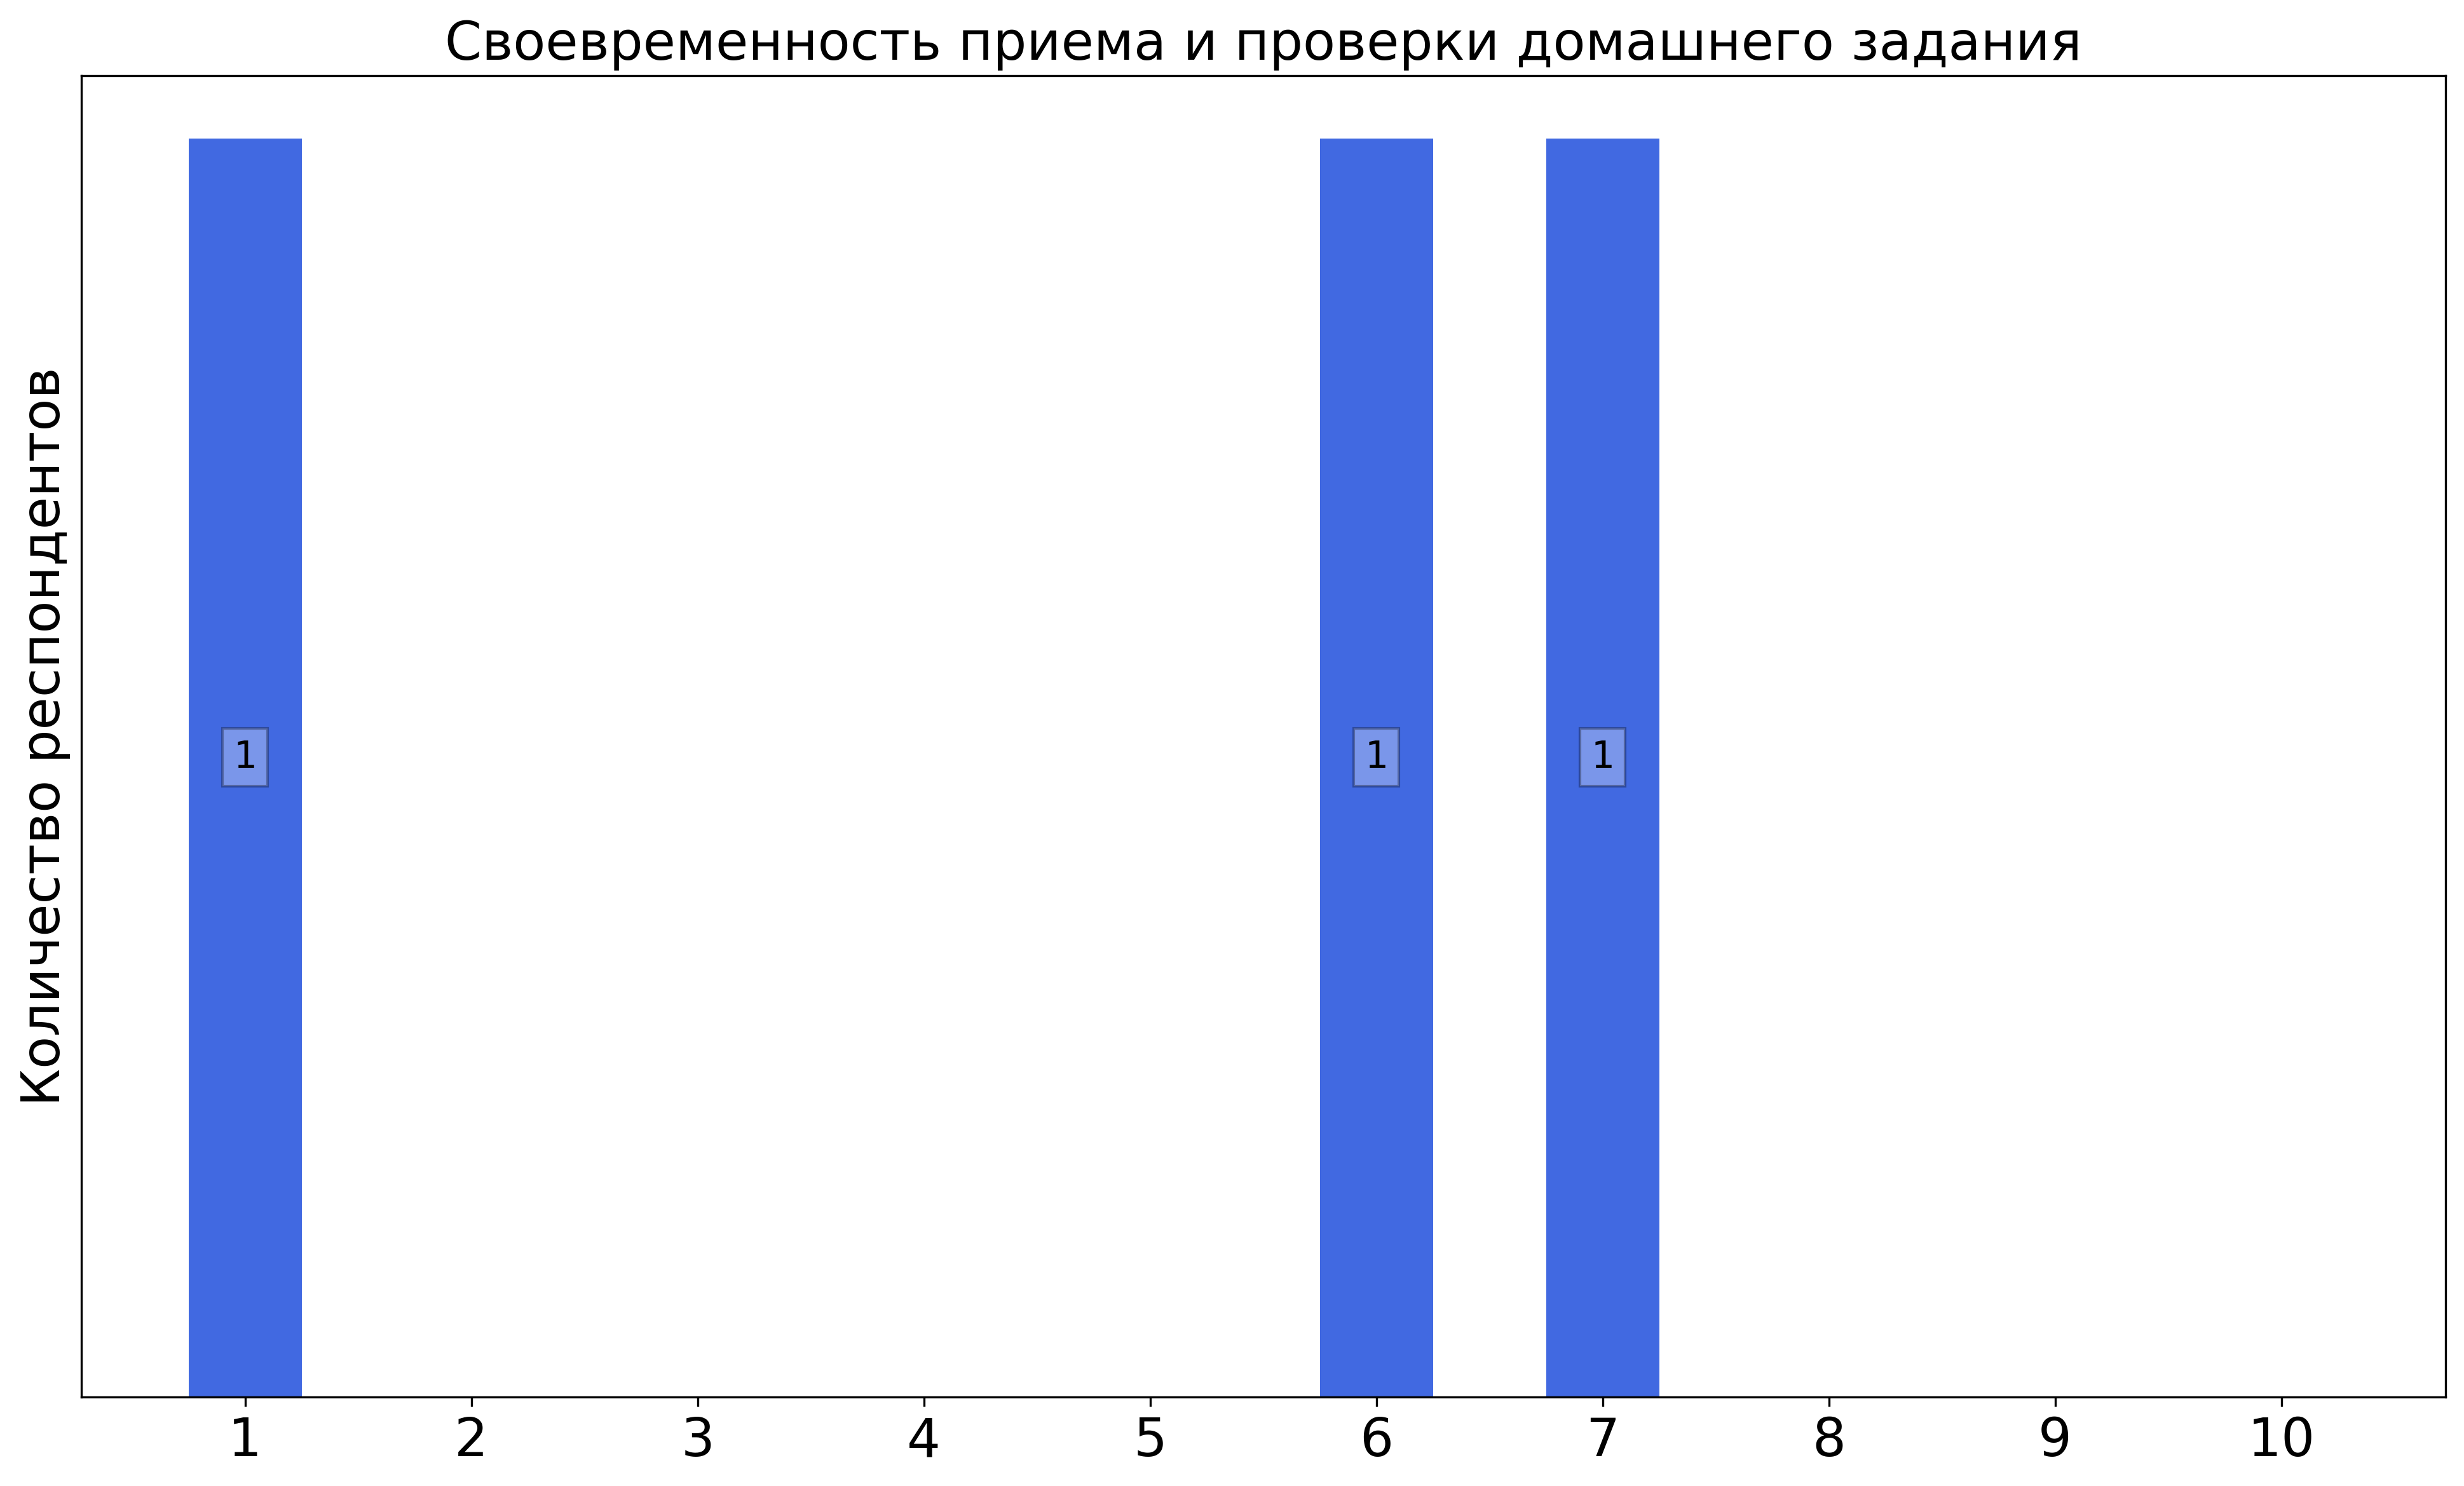
\includegraphics[width=\textwidth]{images/2 course/Компьютерные технологии/seminarists-marks-Чуканова О.В.-2.png}
            \end{subfigure}
            \begin{subfigure}[b]{0.45\textwidth}
                \centering
                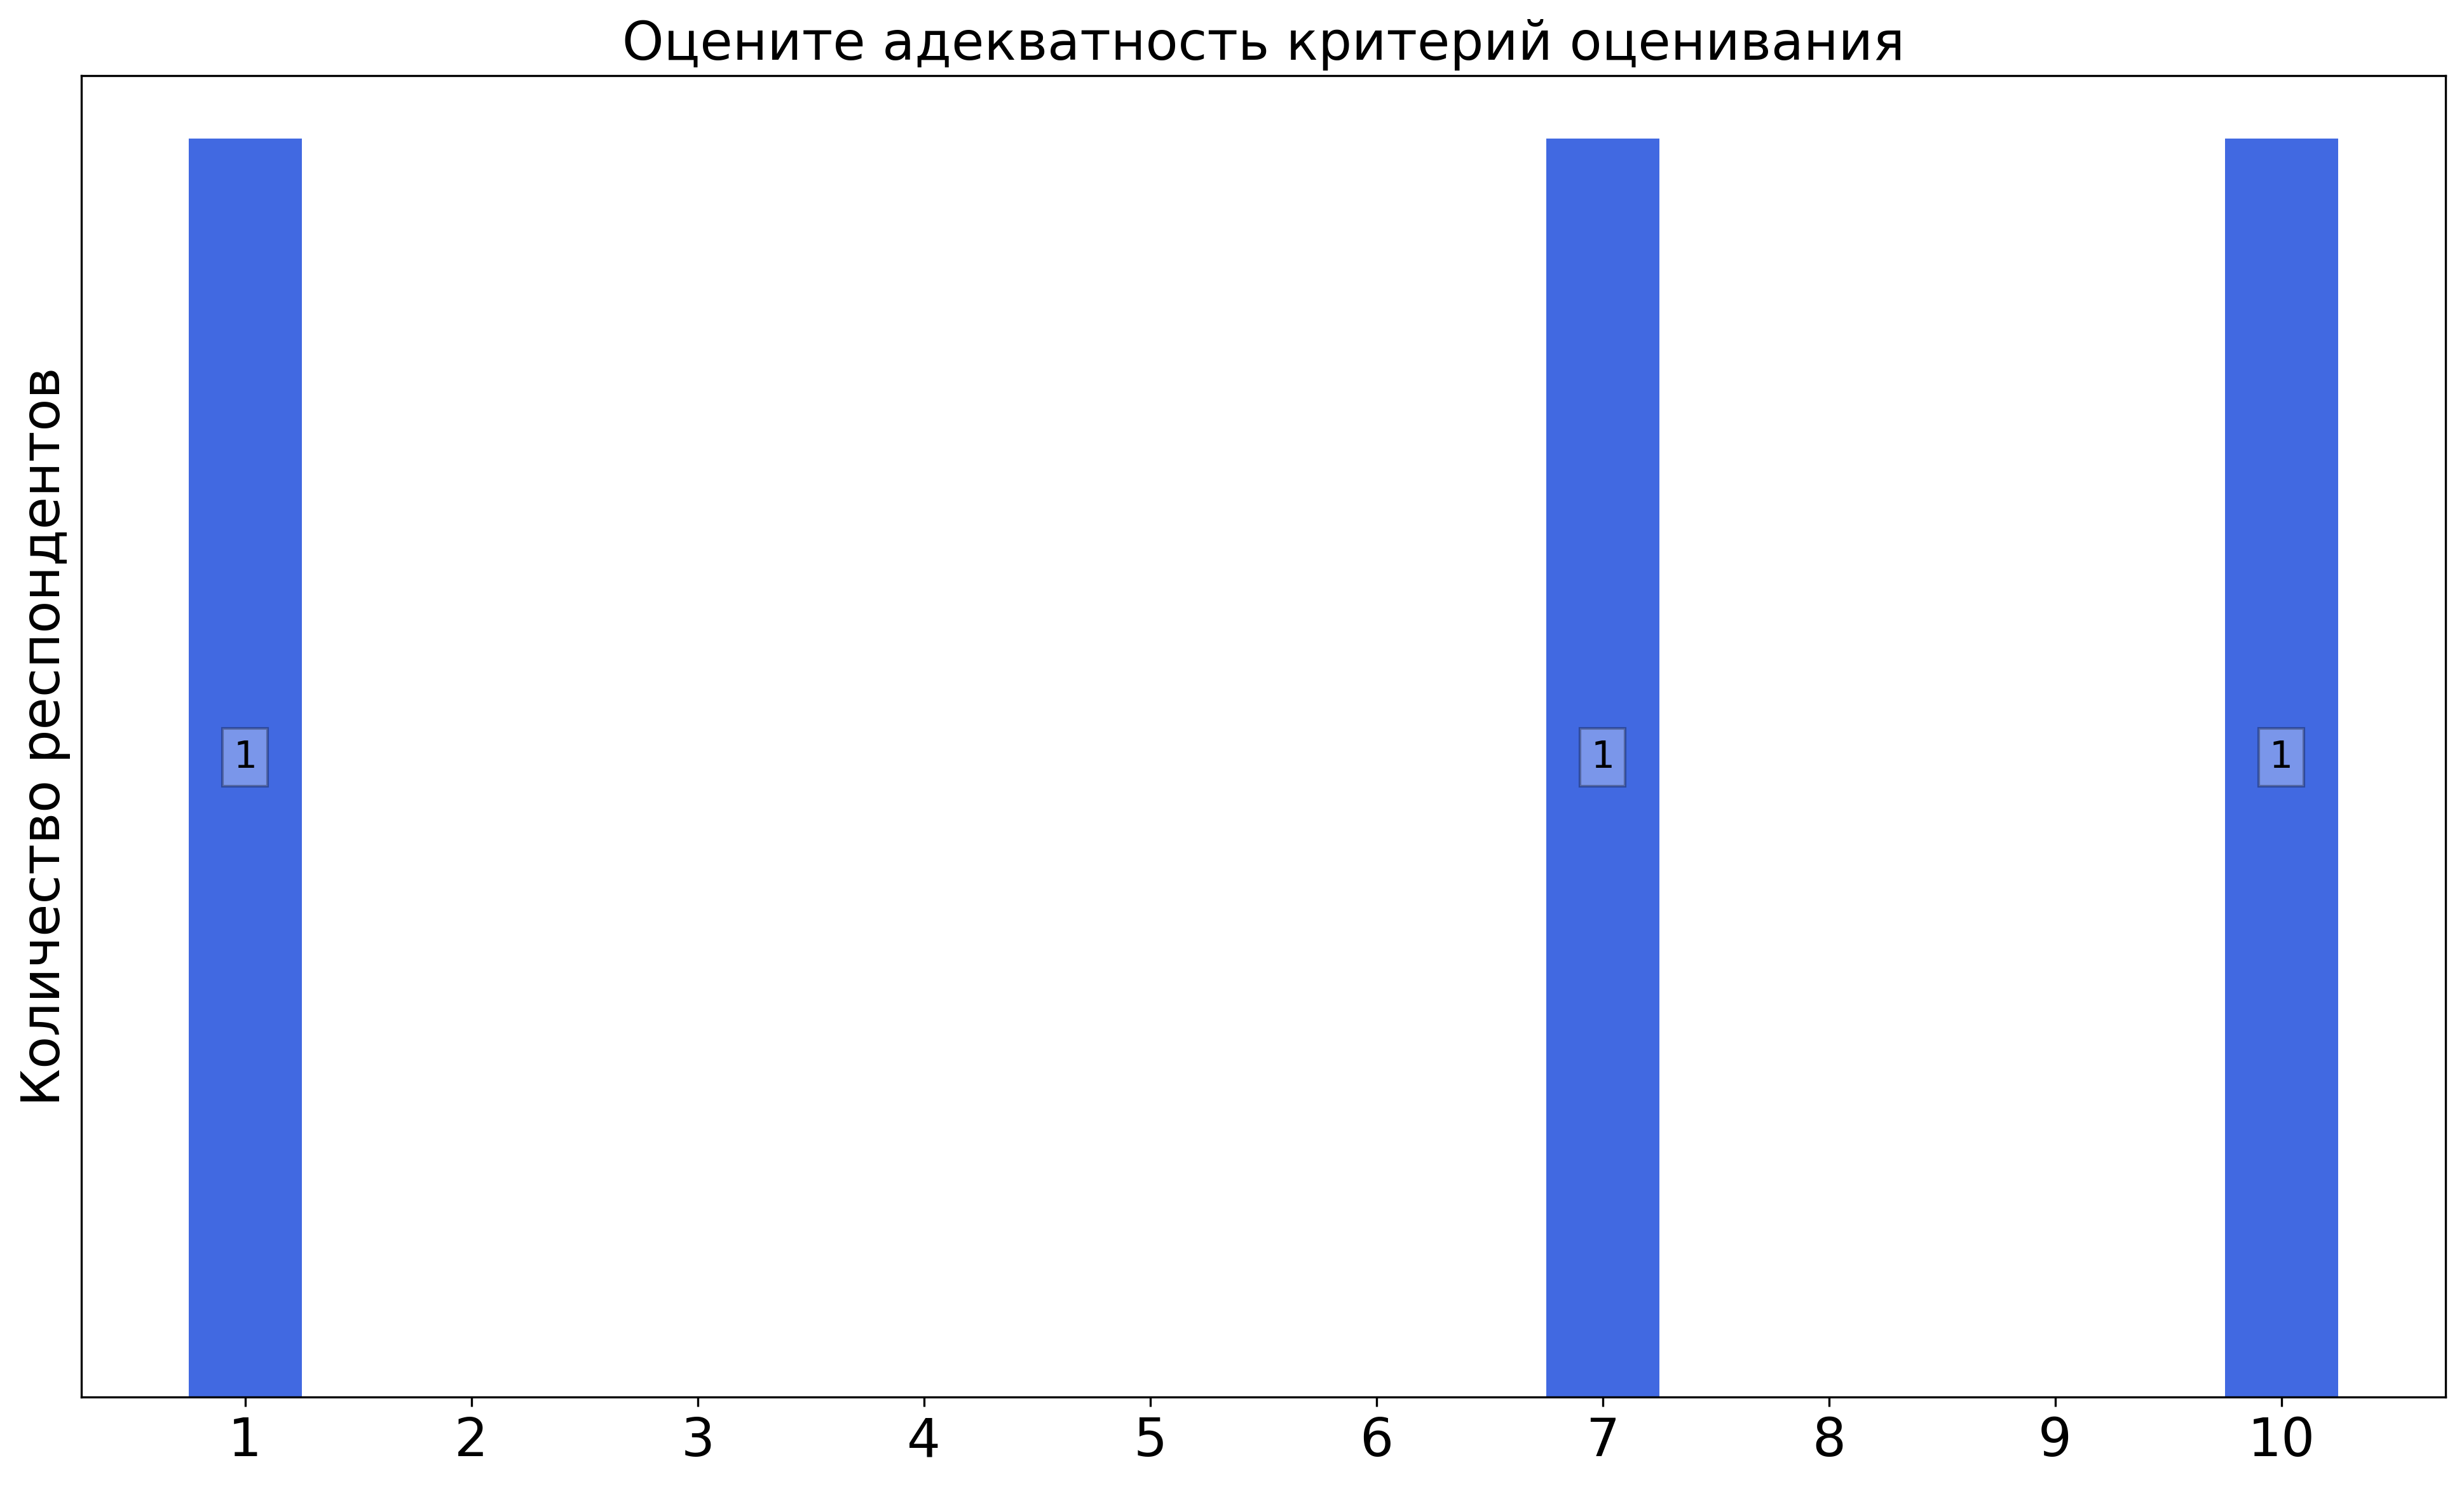
\includegraphics[width=\textwidth]{images/2 course/Компьютерные технологии/seminarists-marks-Чуканова О.В.-3.png}
            \end{subfigure}	
            \caption{Оценки респондентов о качестве преподавания семинаров}
        \end{figure}

        \textbf{Комментарии студентов о семинаристе\protect\footnote{сохранены оригинальные орфография и пунктуация}}
            \begin{commentbox} 
                Внятно курс рассказан не был 
            \end{commentbox} 

    
    \subsubsection{Прочие комментарии и предложения по улучшению курса}

        \begin{commentbox}
            Сделать лекции по информатике не первой парой.
        \end{commentbox}

        \begin{commentbox}
            Очень хотелось бы, чтобы на семинаре хоть один код писали все вместе, чтобы можно было увидеть весь синтаксис и команды, иначе очень много времени уходит на чтение документации, и не всегда вообще знаешь, какие команды удобно использовать.
        \end{commentbox}

        \begin{commentbox}
            Хотелось бы более активные семинары, по поводу лекций написано выше
        \end{commentbox}